\documentclass[mat2, tisk]{fmfdelo}
% \documentclass[fin2, tisk]{fmfdelo}
% \documentclass[isrm2, tisk]{fmfdelo}
% \documentclass[ped, tisk]{fmfdelo}
% Če pobrišete možnost tisk, bodo povezave obarvane,
% na začetku pa ne bo praznih strani po naslovu, …

%%%%%%%%%%%%%%%%%%%%%%%%%%%%%%%%%%%%%%%%%%%%%%%%%%%%%%%%%%%%%%%%%%%%%%%%%%%%%%%
% METAPODATKI
%%%%%%%%%%%%%%%%%%%%%%%%%%%%%%%%%%%%%%%%%%%%%%%%%%%%%%%%%%%%%%%%%%%%%%%%%%%%%%%

% - vaše ime
\avtor{Uroš Kosmač}

% - naslov dela v slovenščini
\naslov{Turbulence v atmosferi in Large eddy simulacije}

% - naslov dela v angleščini
\title{Atmospheric turbulence and Large eddy simulations}

% - ime mentorja/mentorice s polnim nazivom:
%   - doc.~dr.~Ime Priimek
%   - izr.~prof.~dr.~Ime Priimek
%   - prof.~dr.~Ime Priimek
%   za druge variante uporabite ustrezne ukaze
\mentor{prof.~dr.~Emil Žagar}
\somentor{dr.~Peter Smerkol}
% \mentorica{...}
% \somentorica{...}
% \mentorja{...}{...}
% \somentorja{...}{...}
% \mentorici{...}{...}
% \somentorici{...}{...}

% - leto magisterija
\letnica{2025}

% - povzetek v slovenščini
%   V povzetku na kratko opišite vsebinske rezultate dela. Sem ne sodi razlaga
%   organizacije dela, torej v katerem razdelku je kaj, pač pa le opis vsebine.
\povzetek{Tukaj napišemo povzetek vsebine. Sem sodi razlaga vsebine in ne opis tega, kako je delo organizirano.}

% - povzetek v angleščini
\abstract{An abstract of the work is written here. This includes a short description of
the content and not the structure of your work.}

% - klasifikacijske oznake, ločene z vejicami
%   Oznake, ki opisujejo področje dela, so dostopne na strani https://www.ams.org/msc/
\klasifikacija{74B05, 65N99}

% - ključne besede, ki nastopajo v delu, ločene s \sep
\kljucnebesede{integracija\sep kompleks\sep \texorpdfstring{$C^*$}{C*}-algebre}

% - angleški prevod ključnih besed
\keywords{integration\sep complex\sep \texorpdfstring{$C^*$}{C*}-algebras}

% - neobvezna zahvala
%\zahvala{
%  Neobvezno.
%  Zahvaljujem se \dots
%}

% - program dela, ki ga napiše mentor z osnovno literaturo
\programdela{
  Mentor naj napiše program dela skupaj z osnovno literaturo.
}

\osnovnaliteratura{
% Literatura mora biti tukaj posebej samostojno navedena (po pomembnosti) in ne
% le citirana. V tem razdelku literature ne oštevilčimo po svoje, ampak uporabljamo
% ukaz \vnosliterature, v katerega vpišemo citat
  \vnosliterature{wyngaard}
  %\vnosliterature{lebedev2009introduction}
  %\vnosliterature{gurtin1982introduction}
  %\vnosliterature{zienkiewicz2000finite}
  %\vnosliterature{STtemplate}
}

% - ime datoteke z viri (vključno s končnico .bib), če uporabljate BibTeX
\literatura{literatura.bib}

%%%%%%%%%%%%%%%%%%%%%%%%%%%%%%%%%%%%%%%%%%%%%%%%%%%%%%%%%%%%%%%%%%%%%%%%%%%%%%%
% DODATNE DEFINICIJE
%%%%%%%%%%%%%%%%%%%%%%%%%%%%%%%%%%%%%%%%%%%%%%%%%%%%%%%%%%%%%%%%%%%%%%%%%%%%%%%

% naložite dodatne pakete, ki jih potrebujete
\usepackage{units}        % fizikalne enote kot \unit[12]{kg} s polovico nedeljivega presledka, glej primer v kodi
\usepackage{graphicx}     % za slike
\usepackage{graphicx}
\usepackage{subcaption}
\usepackage{tikz}
\usepackage{tikz-3dplot}
\usepackage[utf8]{inputenc}
\usepackage[T1]{fontenc}
\usepackage{lmodern}
\usepackage{amsmath}
\usepackage{amsthm}
\usepackage{amsfonts}
\usepackage{amssymb}
\usepackage{enumitem}
\usepackage{commath}
\usepackage{mathtools}
\usepackage{adjustbox}
\usepackage{setspace}
\usepackage{bigints}
\usepackage{hyperref}
\usepackage{caption}
\usepackage{mathrsfs}
\usepackage[scr=boondoxo]{mathalpha}
\hypersetup{
  colorlinks=true,
  linkcolor=blue,
  urlcolor=cyan,
}
\usepackage{esdiff}
\usepackage{animate}
\usepackage{tikz-cd}
\usepackage{quiver}
\usepackage{nicematrix}
\usetikzlibrary{quotes,arrows.meta}
\usetikzlibrary{decorations.pathreplacing} 
\AtBeginDocument{\hypersetup{pdfborder={0 0 1.1}}}

% VEČ ZANIMIVIH PAKETOV
% \usepackage{array}      % več možnosti za tabele
% \usepackage[list=true,listformat=simple]{subcaption}  % več kot ena slika na figure, omogoči slika 1a, slika 1b
% \usepackage[all]{xy}    % diagrami
% \usepackage{doi}        % za clickable DOI entrye v bibliografiji
% \usepackage{enumerate}     % več možnosti za sezname

% Za barvanje source kode
% \usepackage{minted}
% \renewcommand\listingscaption{Program}

% Za pisanje psevdokode
% \usepackage{algpseudocode}  % za psevdokodo
% \usepackage{algorithm}
% \floatname{algorithm}{Algoritem}
% \renewcommand{\listalgorithmname}{Kazalo algoritmov}

% deklarirajte vse matematične operatorje, da jih bo LaTeX pravilno stavil
% \DeclareMathOperator{\...}{...}

% vstavite svoje definicije ...
\newcommand{\R}{\mathbb R}
\newcommand{\N}{\mathbb N}
\newcommand{\Z}{\mathbb Z}
\newcommand{\bd}{\textbf}
% Lahko se zgodi, da je ukaz \C definiral že paket hyperref,
% zato dobite napako: Command \C already defined.
% V tem primeru namesto ukaza \newcommand uporabite \renewcommand
\newcommand{\C}{\mathbb C}
\newcommand{\Q}{\mathbb Q}

%%%%%%%%%%%%%%%%%%%%%%%%%%%%%%%%%%%%%%%%%%%%%%%%%%%%%%%%%%%%%%%%%%%%%%%%%%%%%%%
% ZAČETEK VSEBINE
%%%%%%%%%%%%%%%%%%%%%%%%%%%%%%%%%%%%%%%%%%%%%%%%%%%%%%%%%%%%%%%%%%%%%%%%%%%%%%%

\begin{document}

\section{Uvod}

\subsection{Motivacija}
Turbulenca oz. turbulentni tok je pojav, s katerim se srečujemo vsak dan, kljub temu pa na nekatera fundamentalna
vprašanja, ki se nanašajo nanjo, še vedno ne znamo odgovoriti. Že vprašanje, kaj je turbulenca, nima
univerzalnega odgovora. So pa opažanja in eksperimenti pokazali, da lahko turbulence
karakteriziramo z določenimi lastnostmi. To so:
\begin{itemize}
\item \textbf{Kaotičnost}: Turbulentni tok je kaotičen oz. nepredvidljiv. To pomeni, če
začetno stanje toka malo spremenimo (spremenimo hitrost, tlak ...), bo končno stanje popolnoma
drugačno, kot pred spremembo. Zato je v praksi zelo težko deterministično napovedati dogajanje.
Teoretično obstajajo Navier-Stokesove enačbe, ki opisujejo gibanje vseh tokov, tudi turbulentnih,
vendar pa je njihovo reševanje zelo zahtevno tudi v posebnih primerih (že sam obstoj rešitev je 
odprto vprašanje).
\item \textbf{Vrtinci različnih velikosti}: Turbulenten tok je sestavljen iz vrtincev (eddies). Lahko so zelo
različnih velikosti, kar je razvidno iz slike \ref{fig:vrtinci}
\begin{figure}[h!]
  \centering
  \begin{subfigure}{.5\textwidth}
    \centering
    \includegraphics[width=0.95\linewidth]{slike/vrtinci.jpeg}
    %\caption{A subfigure}
    %\label{fig:sub1}
  \end{subfigure}%
  \begin{subfigure}{.5\textwidth}
    \centering
    \includegraphics[height=4.58cm, width=0.95\linewidth]{slike/vrtinci2.jpeg}
    %\caption{A subfigure}
    %\label{fig:sub2}
  \end{subfigure}
  \caption{Leva slika prikazuje velike vrtince, ki se pojavijo v atmosferi planeta Jupitra in 
  imajo lahko premer več $1000$ kilometrov, medtem ko desna slika prikazuje turbulenco
  zraka v sobi, kjer se tok zraka prikaže s pomočjo laserja in lahko vidimo vrtince velikosti nekaj mikrometrov.} 
  \label{fig:vrtinci}
  \end{figure}
\item \textbf{Difuzivnost}: Zanimiva lastnost turbuletnega toka je difuzivnost. To pomeni, da se energija in gibalna količina
preneseta po celotnem toku. Osborne Reynolds (1842 - 1912) je postavil eksperiment, ki prikazuje to lastnost. Vidna je
na sliki \ref{fig:difus}
\item \textbf{Reynoldsovo število}: Podoben eksperiment, kot na sliki \ref{fig:difus} nam da enostaven kriterij, ki mu turbulenca zadošča.
Večja kot je dolžina cevi $L$, ali večja kot je hitrost toka $u$, prej bo prišlo do turbulence. Po drugi strani pa večja kot je
viskoznost tekočine $\nu$, manj verjetno bo, da pride do turbulence. To zapišemo preko brezdimenzijske 
konstante $Re = \frac{uL}{\nu}$. Do turbulence pride pri velikih Reynoldsovih številih, običajno pri $Re \geq 5000$.
\item \textbf{Disipativnost}: To je proces prenosa energije iz večjih vrtincev v manjše vrtince, dokler ta ne 
začne izhajati iz tekočine kot toplota. To pomeni, če hočemo imeti turbulenten tok oz. ga ohranjati,
moramo dosledno sistemu dodajati energijo.
\begin{figure}[h!]
  \centering
\includegraphics[scale=0.19]{slike/difus.jpeg}
\caption{V cev polno vode spustimo tok barve. Slika je sestavljena iz treh delov: a) del ni turbulenten zato se barva zalo malo razprši,
b) del je v vmesnem stanju, kjer se že kažejo znaki difuzije in c) del, kjer je tok turbulenten in se barva razširi po celotni cevi.}
\label{fig:difus}
\end{figure}
\begin{figure}[h]
  \centering
\includegraphics[scale=0.19]{slike/Reynolds.jpeg}
\caption{Slika prikazuje hlape plamena, ki potujejo po zraku. Na začetku, imamo majhno Reynoldsovo število, je tok zelo predvidljiv,
ko pa se Reynoldsovo število veča (parameter $L$ se veča), tok postane turbulenten.}
\end{figure}
\end{itemize}

V delu se bom predvsem osredotočil na turbulenco v atmosferi, kjer je obravnava določenih enačb
gibanja in fizikalnih količin nekoliko drugačna, kot pri drugih vrstah turbulence (kot so naprimer turbulence tekočin).
Omejili se bomo na prostor $\R^3$, čeprav bi lahko določene koncepte 
obravnavali v višjih dimenzijah, vendar nam za naše potrebe to ne bo 
prineslo veliko praktične vrednosti.
V splošnem se kakršenkoli tok obravanava na enega od sledečih načinov:
\begin{itemize}
  \item \textbf{Eulerjev pristop}: Recimo, da opazujemo neko domeno $\Omega \subseteq \R^3$, skozi katero teče tok.
  Zanima nas hitrostno polje 
  \begin{align*}
  \textbf{u}: \Omega \times \R^+ &\rightarrow \R^3 \\
  (\bd{x},t) \mapsto&\,\, \textbf{u}(\bd{x},t).
  \end{align*}
  V tem primeru smo fiksirali koordinatni
  sistem (glede na zemljo).
  \item \textbf{Lagrangeev pristop}: Pri tem pristopu opazujemo, s kakšno hitrostjo se delec 
  $\bd{X}$ premika skozi čas. Označimo 
  \begin{align*}
    \bd{X}: \R^+& \rightarrow \R^3 \\
    t \mapsto&\,\, \bd{X}(t; \bd{x}_0),
  \end{align*}
  kjer je $\bd{x}_0$ začetna pozicija delca in 
  velja $\bd{X}(t_0; \bd{x}_0) = \bd{x}_0$.  
  Z drugimi besedami $\bd{X}$ je trajektorija delca, ki se premika skozi čas, tok pa je nabor vseh trajektorij.
\end{itemize}

Kateri pristop uporabimo, je odvisno od lastnosti, ki jih želimo analizirati. Eulerjev pristop
se osredotoči na fiksno domeno in opazujemo kako se lastnosti tekočine spreminjajo v njej skozi čas. 
Za analizo turbulence in globalnih procesov je ta način boljši, medtem ko je Lagrangeva analiza 
boljša za analizo mehanike delcev, disperzije in različnih procesov mešanja (difuzija). 

V delu bomo primarno uporabljali Eulerjev-jev pristop, vendar pa nam lahko analiza enega pomaga
pri analizi drugega. Naj bo $\bd{u}$ Eulerjevo polje hitrosti na poljubni domeni in $X = X(t; \bd{x}_0)$ trajektorija delca 
po Lagrangevem opisu ob času $t$ in začetni pozicija $\bd{x}_0$. 
Zveza med Langrageovo trajektorijo in Eulerjevo hitrostjo je 
\begin{align}
&X(t_0; \bd{x}_0) = \bd{x}_0, \\
\frac{\dif X}{\dif t}&(t; \bd{x}_0) = \bd{u}(X(t; \bd{x}_0), t).
\end{align}
Definiramo Langrangevo polje hitrosti
\begin{equation}
U(t; \bd{x}_0) \coloneqq \bd{u}(X(t; \bd{x}_0), t).
\end{equation}
Poglejmo kako se izraža pospešek delca
\begin{align*}
\frac{\dif}{\dif t} U(t; \bd{x}_0) &= \frac{\partial}{\partial t} \bd{u}(X(t; \bd{x}_0), t) = \\
&= \frac{\dif}{\dif t} X(t; \bd{x}_0) \cdot \Big(\text{grad}_\bd{x} \bd{u}(\bd{x}, t) \Big)_{\bd{x} = X(t, \bd{x}_0)} + \Big(\frac{\partial}{\partial t} \bd{u}(\bd{x}, t) \Big)_{\bd{x} = X(t, \bd{x}_0)} = \\
&= \Big(\bd{u}(t; \bd{x}_0) \cdot \text{grad}_\bd{x} \bd{u}(\bd{x}, t) + \frac{\partial}{\partial t} \bd{u}(\bd{x}, t) \Big)_{\bd{x} = X(t, \bd{x}_0)}.
\end{align*}

\newpage
\begin{definicija}
Naj bo $\Omega \subset \R^n$ in $\bd{v}: \Omega\times \R^+ \rightarrow \R^n$ vektorsko polje. Diferencialni operator 
$\frac{D}{D t}: C^1(\Omega \times \R^+, \R^n) \rightarrow C^0(\Omega \times \R^+, \R^n)$ dan s predpisom
\begin{equation}
\frac{D \bd{u}}{Dt} = \Big(\frac{\partial}{\partial t} + \bd{v} \cdot \nabla_\bd{x}\Big) \bd{u} = \frac{\partial \bd{u}}{\partial t} + (v\cdot \nabla_x) u
\end{equation}
se imenuje \textbf{materialni odvod}.
\end{definicija}

Pospešek, zapisan preko materialnega odvoda je 
\begin{equation}
\frac{\dif}{\dif t} U(t; \bd{x}_0) = \Big(\frac{D \bd{u}}{Dt}(\bd{x}, t) \Big)_{\bd{x} = X(t; \bd{x}_0)}.
\end{equation}

Podoben rezultat dobimo, če namesto hitrosti, odvajamo gostoto
\begin{equation}
\frac{\dif }{\dif t} P(t; \bd{x}_0) = \Big(\frac{D \rho}{Dt}(x, t) \Big)_{\bd{x} = X(t; \bd{x}_0)}.
\end{equation}
Materialni odvod je fundementalni operator Eulerjevaga pristopa. Vedno, ko nas bo 
zanimalo kako se neka količina spreminja s časom, nas bo zanimal njen materialni odvod.

\begin{opomba}
Operator $\nabla$ ni komutativen. Za vektorsko polje $\bd{v}$ : $\bd{v} \cdot \nabla \neq \nabla \cdot \bd{v}$.
\end{opomba}


\subsection{Ohranitveni zakoni}

V tem razdelku začnemo matematični opis enega najbolj pomembnih konceptov dinamike fluidov (in fizike na splošno), 
ki je ključen za razumevanje turbulentnih tokov. 

\begin{opomba}
V nadaljevanju ne bomo navajali vseh potrebnih predpostavk, ki bodo upravičile naše izpeljave. Na primer 
\begin{itemize}
  \item Domene, s katerimi bomo imeli opravka, bodo gladke orientabilne mnogoterosti.
  \item Vektorska polja bodo gladka, v naslednjem poglavju pa bomo predpostavili, da 
  obstaja razvoj v Fourierovo vrsto.
  \item Menjave vrstnega reda limit bo potrebno upravičiti, zato bomo zahtevali, da je 
  vektorsko polje $\bd{u}$ tudi v $L^2$ prostoru.
\end{itemize}
\end{opomba}

\subsubsection{Zakon o ohranitvi mase}
Naj bo $\Omega \subseteq \R^3$ omejena, $\partial \Omega$ njen rob in $\rho: \Omega \times [0, \infty) \rightarrow [0, \infty)$ 
gostota množice $\Omega$, ki je gladka. Masa $m$ od $\Omega$ je 
\begin{equation}
  m(\Omega) = \int_\Omega \rho(\bd{x}, t) \dif V.
\end{equation}
\begin{center}
\begin{tikzpicture}
  \draw  plot[smooth, tension=.7] coordinates {(-3.5,0.5) (-3,2.5) (-1,3.5) (1.5,3) (4,3.5) (5,2.5) (5,0.5) (2.5,-2) (0,-0.5) (-3,-2) (-3.5,0.5)};
  \draw[thick, rotate = 30] (-1.3,0.8) ellipse (0.4 and 0.7);
  \filldraw[red, rotate = 30] (-1.3,0.8) circle(2pt) ;
  \draw[thick, red, rotate = 30, ->] (-1.3,0.8) -- (-3,0.7) node[above, black] {$\bd{u}$};
  \node at (1.5,1.5) {$\Omega$};
  \node at (4,4) {$\partial$$\Omega$};
\end{tikzpicture}
\end{center}
~\\[1mm]

Zakon o ohranitvi mase pravi, da je količina mase, ki se pretoči v $\Omega$ v določenem času, 
enaka količini mase, ki se iztoči skozi $\partial\Omega$ tj.
$$
\frac{\partial m}{\partial t} = - \int_{\partial \Omega} \rho\bd{u} \dif \bd{S}.
$$
Ker je domena $\Omega$ končna in $\rho$ gladka lahko zamenjamo vrstni red odvajanja in integriranja
$$
\int_\Omega \frac{\partial}{\partial t} \rho(x, t) \dif V = - \int_{\partial \Omega} \rho \bd{u} \dif \bd{S}.
$$
Izrek o divergenci pravi, da je:
$$
\int_{\partial \Omega} \rho\bd{u} \dif \bd{S} = \int_{\Omega} \nabla \cdot (\rho\bd{u}) \dif V
$$
Dobimo 
\begin{align*}
\int_\Omega \left(\frac{\partial}{\partial t} \rho(x, t) + \nabla \cdot (\rho\bd{u})\right) \dif V = 0.
\end{align*}

Naslednja lema nam bo povedala, da je integrand enak 0.

\begin{lema}
  \label{lema:1}
Naj bo $f: \Omega \subset \R^n \rightarrow \R$ zvezna. 
Če za vsako podmnožico $\Omega' \subset \Omega$ velja 
$$
\int_{\Omega'} f(\bd{x}) \dif V = 0,
$$
potem je 
$$
f(\bd{x}) = 0, \quad \forall \bd{x} \in \Omega.
$$
\end{lema}

\begin{dokaz}
Recimo, da je $f(\bd{x}_0) \neq 0$ za $\bd{x}_0 \in \Omega' \subset \Omega$. Brez škode 
splošnosti predpostavimo $f(\bd{x}_0) > 0$. Zaradi 
zveznosti funkcije $f$ obstaja tak $\delta > 0$, da je 
$$
f(\bd{x}) > 0, \quad \forall \bd{x} \in B(\bd{x}_0, \delta) \subset \Omega'.
$$
Integriramo nenegativno funkcijo 
$$
\int_{\Omega'} f(\bd{x}) \dif V = \int_{B(\bd{x}_0, \delta)} f(\bd{x}) \dif V > 0.
$$
To vodi je protislovje, torej je $f(\bd{x}) = 0$.
\end{dokaz}

Ker enakost velja za vsako domeno $\Omega$ iz leme sledi enakost
\begin{equation}
\frac{\partial \rho}{\partial t} + \nabla \cdot (\rho\bd{u}) = 0.
\end{equation}


To je diferencialna oblika zakona o ohranitvi mase, enačbi, ki zakon opiše, pravimo \textbf{kontinuitetna enačba}.
Če je gostota konstantna, tj. $\rho(x, t) \equiv c > 0$, potem se kontinuitetna enačba poenostavi
$$
\frac{\partial \rho}{\partial t} + \nabla \cdot (\rho\bd{u}) = \rho (\nabla \cdot \bd{u}) = 0 \Longrightarrow \nabla \cdot u = 0.
$$
\begin{definicija}
Tok je \textbf{nestisljiv}, če velja 
\begin{equation}
\label{ohranitev mase}
  \nabla \cdot u = 0.    
\end{equation}
\end{definicija}

\subsection{Zakon o ohranitvi gibalne količine}
V tem razdelku bomo predpostavili, da je gostota $\rho$ konstantna, tj.
\begin{equation}
m = \int_\Omega \rho \dif V = \rho \int_\Omega \dif V = \rho \cdot V,
\end{equation}
kjer je $V = \int_\Omega \dif V$ volumen domene $\Omega$. Zakon o ohranitvi gibalne količine, 
pravi, da je vsota gibalnih količin ($\bd{p}$) v zaprtem sistemu konstanten. Za $n$ delcev je
\begin{align*}
&\sum_{k=1}^n \bd{p}_k = \text{const.} \\[1mm]
&\sum_{k=1}^n \frac{\dif \bd{p}_k}{\dif t} = 0.
\end{align*}
Gibalna količina je dana s $\bd{p} = m \bd{v}$, kar ekvivalentno zapišemo
\begin{align*}
\frac{\dif \bd{p}}{\dif t} = \frac{\dif \,(m \bd{v})}{\dif t} &= m\frac{\dif \bd{v}}{\dif t} = m \bd{a} = \bd{F} \Longrightarrow\\[2mm]
\sum_{k=1}^n \bd{F}_k &= 0.
\end{align*}
To je ravno 1. Newtonov zakon. Ob upoštevanju 2. Newtonov zakona, dobimo obliko:
\begin{equation}
\sum_{k=1}^n \bd{F}_k = m \bd{a}.
\end{equation}
Zapišimo ta zakon za tokove, preko materialnega odvoda.
\begin{align*}
m \bd{a} = \rho V \frac{D \bd{u}}{D t} = \sum_{k=1}^n \bd{F}_k \\
\rho \frac{D \bd{u}}{D t} = \sum_{k=1}^n \frac{\bd{F}_k}{V}. 
\end{align*}
Pri tokovih se pojavita dve vrsti sil 
\begin{itemize}
  \item Ploskovne sile, ki jih delimo na 
  \begin{enumerate}
    \item[1)] Tangencialne (viskoznost)
    \item[2)] Normalne (tlak)
  \end{enumerate}
  \item Telesne oz. zunanje sile (gravitacija, Coriolisova sila, magnetizem, \dots)
\end{itemize}
Izraz $\frac{F_k}{V}$ bomo zapisali preko količin $\bd{u}$ in $p$. 
Izpeljave naredimo v enodimenzionalnem primeru, kar se enostavno posploši 
na višje dimenzije.\\
\textbf{Normalna sila .oz tlak:}\\[1mm]
\begin{center}

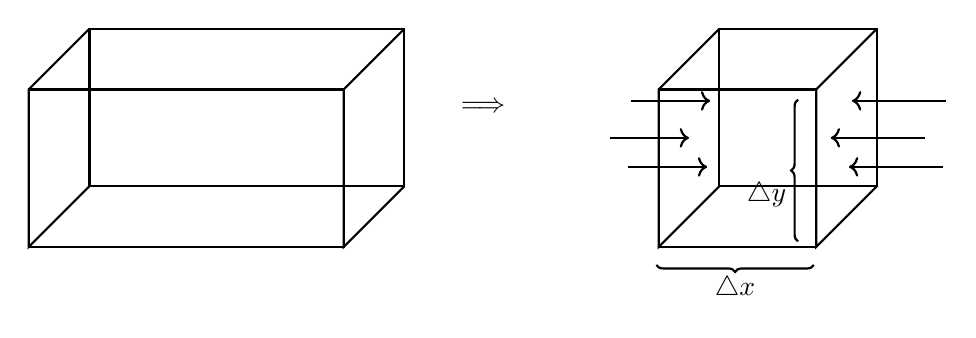
\begin{tikzpicture}[scale=2]
  \draw[thick] (-4,0,0) -- (-2,0,0) -- (-2,1,0) -- (-4,1,0) -- cycle; % Bottom face
  \draw[thick] (-4,0,0) -- (-4,0,1) -- (-4,1,1) -- (-4,1,0);          % Left face
  \draw[thick] (-2,0,0) -- (-2,0,1) -- (-2,1,1) -- (-2,1,0);          % Right face
  \draw[thick] (-4,0,1) -- (-2,0,1) -- (-2,1,1) -- (-4,1,1) -- cycle; % Top face

  \draw[thick] (0,0,0) -- (1,0,0) -- (1,1,0) -- (0,1,0) -- cycle; % Bottom face
  \draw[thick] (0,0,0) -- (0,0,1) -- (0,1,1) -- (0,1,0);          % Left face
  \draw[thick] (1,0,0) -- (1,0,1) -- (1,1,1) -- (1,1,0);          % Right face
  \draw[thick] (0,0,1) -- (1,0,1) -- (1,1,1) -- (0,1,1) -- cycle; % Top face

  % Left arrow
  \draw[->, thick] (-0.5, 0.2, 0.2) -- (0, 0.2, 0.2);
  \draw[->, thick] (-0.5, 0.5, 0.5) -- (0, 0.5, 0.5);
  \draw[->, thick] (-0.5, 0.6, 0.15) -- (0, 0.6, 0.15);

  % Right arrow
  \draw[->, thick] (1.5, 0.2, 0.2) -- (0.9, 0.2, 0.2);
  \draw[->, thick] (1.5, 0.5, 0.5) -- (0.9, 0.5, 0.5);
  \draw[->, thick] (1.5, 0.6, 0.15) -- (0.9, 0.6, 0.15);

  %\draw[->, thick] (0.9, 1.9, 1.5) -- (0.9, 1.4, 1.5);
  %\draw[->, thick] (1.2, 1.9, 1.7) -- (1.2, 1.4, 1.7);
  %\draw[->, thick] (0.6, 1.9, 1.7) -- (0.6, 1.4, 1.7);

  \node at (-1.5, 0.5, 0) {$\Longrightarrow$};
  %\node at (0.5, -0.5, 0) {Front};
  \draw[thick, decorate, decoration={brace, mirror}] (-0.4, -0.5, 0) -- (0.6, -0.5, 0) 
        node[midway, yshift=-0.3cm] {$\triangle x$};
  \draw[thick, decorate, decoration={brace}] (0.5, -0.35, 0) -- (0.5, 0.55, 0) 
        node[midway, xshift = -0.4cm, yshift=-0.3cm] {$\triangle y$};
\end{tikzpicture}
\end{center}

Recimo, da imamo majhno pravokotno domeno z volumnom $V = \triangle x \triangle y  \triangle z$.
Poglejmo, kako se sila izraža v $x$ - smeri, ko pride do spremembe tlaka. Ta je definiran kot $p = \frac{\triangle F}{\triangle A}$, 
kjer sta $\triangle F$ - majhna sprememba sile in $\triangle A$ - majhna sprememba površine. Imamo:
\begin{align*}
F_x &= p_1 A_1 - p_2 A_2 = \quad \quad(A_1 = A_2 = A) \\
F_x &= (p_1 - p_2)A = \triangle p A \quad \Longrightarrow \\
\frac{F_x}{V} &= \frac{\triangle p \triangle y \triangle z}{\triangle x \triangle y \triangle z} = \frac{\triangle p}{\triangle x}
\end{align*}
Pošljemo $\triangle x$ proti $0$:
$$
\frac{F}{V} = \lim_{\triangle x \rightarrow 0 }\frac{F_x}{V} = \lim_{\triangle x \rightarrow 0} \frac{\triangle p}{\triangle x} = \frac{\partial p}{\partial x}
$$
Na enak način dobimo v $y$ in $z$ smeri. V vektorskem zapisu: 
$\frac{\bd{F}}{V} = \nabla p$.
\noindent
\textbf{Tangencialna sila oz. viskoznost:} \\[1mm]
Viskoznost ima podobno vlogo kot koeficient trenje. To je merilo za koliko tekočina 
„ustavlja“ samo sebe. Sila med tokovoma, ki je posledica 
premikanja oz. drsenja med njima imenujemo strižna napetost. Definirana je enako kot tlak, vendar kaže v drugo smer, tj. $\tau = \frac{F}{A}$.
\begin{center}
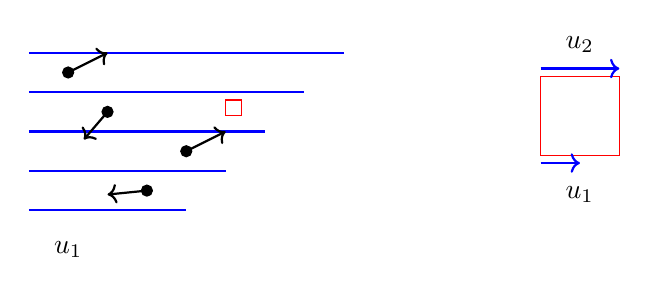
\begin{tikzpicture}
  % Draw horizontal blue lines of different lengths
  \draw[thick, blue] (0,2) -- (4,2);
  \draw[thick, blue] (0,1.5) -- (3.5,1.5);
  \draw[thick, blue] (0,1) -- (3,1);
  \draw[thick, blue] (0,0.5) -- (2.5,0.5);
  \draw[thick, blue] (0,0) -- (2,0);
  
  % Add atoms as small circles
  \filldraw[black] (1.5,0.25) circle(2pt) node[below] {};
  \filldraw[black] (2,0.75) circle(2pt) node[below] {};
  \filldraw[black] (1,1.25) circle(2pt) node[below] {};
  \filldraw[black] (0.5,1.75) circle(2pt) node[below] {};
  
  % Add arrows for the motion of atoms
  \draw[->, thick] (1.5,0.25) -- (1,0.2);
  \draw[->, thick] (2,0.75) -- (2.5,1);
  \draw[->, thick] (1,1.25) -- (0.7,0.9);
  \draw[->, thick] (0.5,1.75) -- (1,2);
  
  % Add a small red square
  \draw[red] (2.5,1.2) rectangle +(0.2,0.2);
  
  
  \draw[red] (6.5,0.7) rectangle +(1,1);
  \draw[->, thick, blue] (6.5,0.6) -- (7,0.6);
  \draw[->, thick, blue] (6.5,1.8) -- (7.5,1.8);
  \node at (0.5, -0.5, 0) {$u_1$};

  % Add labels
  \node at (7.3,2.1) [left] {$u_2$};
  \node at (7.3,0.2) [left] {$u_1$};
\end{tikzpicture}
\end{center}
Pogledamo spremembo hitrosti v $x$ - smeri
$$
\tau_x = \frac{F_x}{A} = \frac{m}{A} \cdot \frac{\triangle u}{\triangle t}\cdot \frac{\triangle y}{\triangle y} = \underbrace{\frac{m}{A} \cdot\frac{\triangle y}{\triangle t}}_{\mu} \cdot\frac{\triangle u}{\triangle y} = \mu \frac{\triangle u}{\triangle y}.
$$
$\mu$ je dinamična viskoznost, odvisna le od lastnosti tekočine. 
Ko pošljemo $\triangle y \rightarrow 0$, dobimo
$$
\tau = \lim_{\triangle y \rightarrow 0} \tau_x = \lim_{\triangle y \rightarrow 0} \mu\frac{\triangle u}{\triangle y} = \mu\frac{\partial u}{\partial y}
$$
Naredimo podobno analizo, kot pri tlaku \\
\begin{center}
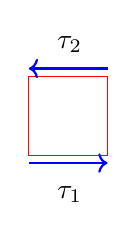
\begin{tikzpicture}
  \draw[red] (3.5,0.7) rectangle +(1,1);
  \draw[->, thick, blue] (3.5,0.6) -- (4.5,0.6);
  \draw[->, thick, blue] (4.5,1.8) -- (3.5,1.8);

  % Add labels
  \node at (4.3,2.1) [left] {$\tau_2$};
  \node at (4.3,0.2) [left] {$\tau_1$};
\end{tikzpicture}
\end{center}
Če sta strižni napetosti različni, imamo neničelno silo na majhnem območju $\Omega = \triangle x \triangle y \triangle z$:
\begin{align*}
F_x &= \tau_2 A_2 - \tau_1 A_1  \quad (A_1 = A_2)\\
F_x &= \triangle \tau \triangle x \triangle z  \quad \Longrightarrow\\
\frac{F_x}{V} &= \frac{\triangle \tau \triangle x \triangle z}{\triangle x \triangle y \triangle z} = \frac{\triangle \tau}{\triangle y}.
\end{align*}
Ponovno pošljemo $\triangle y \rightarrow 0$
$$
\frac{F}{V} = \lim_{\triangle y \rightarrow 0} \frac{F_x}{V} = \lim_{\triangle y \rightarrow 0} \frac{\triangle \tau}{\triangle y} = \frac{\partial \tau}{\partial y} = \frac{\partial}{\partial y} \Big(\mu\frac{\partial u}{\partial y} \Big) = \mu \frac{\partial^2 u}{\partial y^2}.
$$
Delec volumna se premika le v $x$ - smeri, vendar strižna napetost deluje na vse njegove površine, zato, je sila izraža preko Laplaceovega operatorja
$$
\frac{F}{V} = \mu \Big(\frac{\partial^2 u}{\partial x^2} + \frac{\partial^2 u}{\partial y^2} + \frac{\partial^2 u}{\partial z^2} =  \Big) = \mu \nabla^2 u.
$$
V vektorski notaciji: $\frac{\bd{F}}{V} = \mu \nabla^2 \bd{u}$.\\
\textbf{Telesne sile:} \\
V splošnem je veliko različnih sil, tu pa bomo upoštevali le gravitacijo (v modeliranju atmosfere, je ključno, da upoštevamo Corioliosovo silo). Gravitacijska sila v primeru tokov 
$$
\frac{\bd{F}}{V} = \frac{m \bd{g}}{V} = \frac{\rho V \bd{g}}{V} = \rho \bd{g}.
$$
Ko združimo vse tri sile, dobimo enačbo
$$
\rho \frac{D u}{D t} = - \frac{\partial p}{\partial x} + \mu \Big( \frac{\partial^2 u}{\partial x^2} + \frac{\partial^2 u}{\partial y^2} + \frac{\partial^2 u}{\partial z^2} \Big) + \rho g.
$$
Ker je hitrost vektorska količina, imamo $3$ enačbe 
\begin{align*}
  \rho \frac{D u}{D t} &= - \frac{\partial p}{\partial x} + \mu \Big( \frac{\partial^2 u}{\partial x^2} + \frac{\partial^2 u}{\partial y^2} + \frac{\partial^2 u}{\partial z^2} \Big) + \rho g_x,\\
  \rho \frac{D v}{D t} &= - \frac{\partial p}{\partial y} + \mu \Big( \frac{\partial^2 v}{\partial x^2} + \frac{\partial^2 v}{\partial y^2} + \frac{\partial^2 v}{\partial z^2} \Big) + \rho g_y,\\
  \rho \frac{D w}{D t} &= - \frac{\partial p}{\partial z} + \mu \Big( \frac{\partial^2 w}{\partial x^2} + \frac{\partial^2 w}{\partial y^2} + \frac{\partial^2 w}{\partial z^2} \Big) + \rho g_z.
\end{align*}
Kompaktno zapišemo 
$$
\rho \frac{D \bd{u}}{D t} = - \nabla p + \mu \nabla^2 \bd{u} + \rho \bd{g},
$$
kjer sta $\bd{u} = (u, v, w)$ in $g = (g_x, g_y, g_z)$. Tem enačbam pravimo Navier-Stokesove enačbe.
Običajno se zadnjo enačbo deli z gostoto $\rho$ in uvede \textbf{kinematično viskoznost} $\nu = \frac{\mu}{\rho}$. Če razpišemo
 materialni odvod, se celotna enačba glasi
\begin{equation}
  \label{NS}
\frac{D \bd{u}}{D t} = \frac{\partial \bd{u}}{\partial t} + (\bd{u}\cdot \nabla)\bd{u} = - \frac{1}{\rho}\nabla p + \nu \nabla^2 \bd{u} + \rho \bd{g}.
\end{equation}

\begin{opomba}
  \hfil
\begin{itemize}
  \item Če ne poznamo telesnih sil ali jih imamo več, v zadnji enačbi sumand $\rho \bd{g}$ zamenjamo s $\bd{f}$.
  \item Količine deljene z gostoto, imenujemo kinematične količine.
\end{itemize}
\end{opomba}

\subsection{Zakon o ohranitvi vrtinčnosti}

Naslednja pomembna količina je vrtinčenja \bd{$\omega$}. Kot že ime pove, je to količina, ki opisuje vrtenje toka okoli neke točke. 
\begin{definicija}
Naj bo $\bd{u} \in C^1(\Omega)$, $\Omega \subset \R^3$ . Vrtinčenje $\omega$ je rotor polja $\bd{u}$
\begin{equation}
\bd{$\omega$} \equiv \nabla \times \bd{u}.
\end{equation}
\end{definicija}
Ohranitveno enačbo za \bd{$\omega$} dobimo preko Navier-Stokesove enačbe. Predpostavimo, 
da je vektorsko polje $\bd{u} \in C^2$ na poljubni domeni. Vzamemo rotor enačbe \eqref{NS}:
\begin{align*}
\nabla \times (\frac{\partial \bd{u}}{\partial t} + (\bd{u}\cdot \nabla)\bd{u}) = \nabla\times (- \frac{1}{\rho}\nabla p + \nu \nabla^2 \bd{u} + \bd{f}) \\
\frac{\partial \bd{$\omega$}}{\partial t} + \nabla \times ((\bd{u}\cdot \nabla)\bd{u}) = - \frac{1}{\rho} \nabla \times (\nabla p) + \nu\nabla^2 \bd{$\omega$} + \nabla \times \bd{f}
\end{align*}
Dobro znano dejstvo je, da je rotor gradienta skalarne funkcije $0$, torej je 
$\nabla \times (\nabla p) = \bd{0}$. Poenostavimo člen s hitrostjo. Iz dvojnega vektorskega produkta dobimo 
\begin{align*}
\bd{u} \times (\nabla \times \bd{u}) &=  \nabla(\bd{u}\cdot \bd{u}) - (\bd{u}\cdot \nabla)\bd{u} \\
\Longrightarrow \quad(\bd{u}\cdot \nabla)\bd{u} &= \nabla (\bd{u}\cdot \bd{u}) - \bd{u}\times (\underbrace{\nabla \times \bd{u}}_{= \bd{$\omega$}})
\end{align*}
Vzamemo rotor zadnje enakosti:
\begin{align*}
\nabla \times (\bd{u}\cdot \nabla)\bd{u} &= \underbrace{\nabla \times (\nabla(\bd{u}\cdot \bd{u}))}_{= 0} - \nabla \times (\bd{u} \times \bd{$\omega$}) \\
&= \nabla \times (\bd{$\omega$} \times \bd{u}) \\
&= (\bd{u}\cdot \nabla)\bd{$\omega$} - (\bd{$\omega$} \cdot \nabla)\bd{u} + \bd{$\omega$}\underbrace{(\nabla \cdot \bd{u})}_{= 0 \text{ po } \eqref{ohranitev mase}} + \bd{u} \underbrace{(\nabla \cdot \bd{$\omega$})}_{= 0}
\end{align*}
Vstavimo v prvotno enačbo
\begin{align*}
\frac{\partial \bd{$\omega$}}{\partial t} + (\bd{u}\cdot \nabla)\bd{$\omega$} + (\bd{$\omega$} \cdot \nabla)\bd{u} - (\bd{$\omega$} \cdot \nabla)\bd{u} + \bd{u} (\nabla \cdot \bd{$\omega$}) =  \nu\nabla^2 \bd{$\omega$} + \nabla \times \bd{f}.
\end{align*}
Enačba, ki opiše zakon
\begin{equation}
\frac{D\bd{$\omega$}}{D t} = \frac{\partial \bd{$\omega$}}{\partial t} + (\bd{u}\cdot \nabla)\bd{$\omega$} = (\bd{$\omega$} \cdot \nabla)\bd{u}+ \nu \nabla^2 \bd{$\omega$} + \nabla \times \bd{f}.
\end{equation}

\subsection{Zakon o ohranitvi skalarja}
Sedaj bomo posplošili zakon o ohranitvi mase, za poljubno zvezno odvedljivo skalarno polje $c: \Omega \times \R^+ \rightarrow \R$ na 
$\Omega \subset \R^3$.
Začnemo z enako enačbo kot pri zakonu o ohranitvi mase, le, da dodamo še dva dodatna 
člena. Ta člena sta $F$ - vektorsko polje, za pretok oz. prenos skalarja $c$ in $H$ - izvor za skalar $c$.
V integralski obliki zapišemo:
\begin{equation}
\frac{\dif}{\dif t} \int_{\Omega} c \dif V = - \int_S \bd{F} \cdot \dif \bd{S} - 
\int_S c \bd{u}  \dif \bd{S} + \int_\Omega H \dif V,
\end{equation}
kjer je $S = \partial \Omega$.
Prva dva člena imata negativen predznak, ker skalar odteka. Če je $H < 0$ potem imamo odtok skalarja, če pa je $H > 0$ imamo pritok skalarja. 

\begin{primer}
Enostaven primer, ki pokaže pomen količine $H$. Pri zgornji luknji imamo pritok 
mase (tekočine) in v tem primeru je $H_{p} > 0$, med tem, ko imamo v spodnji luknji odtok
mase (tekočine) in je $H_{0} > 0$. Celotni $H$ je razlika $H = H_p - H_0$.\\
\begin{center}
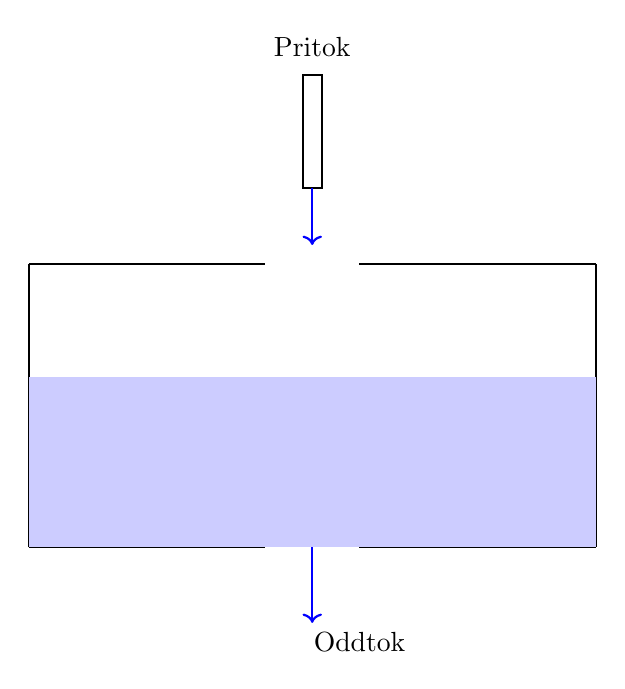
\begin{tikzpicture}[scale=1.2]

  % Basin (korito) with gaps at the bottom and top
  \draw[thick] (0,0) -- (2.5,0);    % Left part of bottom line
  \draw[thick] (3.5,0) -- (6,0);    % Right part of bottom line
  
  \draw[thick] (0,3) -- (2.5,3);    % Left part of top line
  \draw[thick] (3.5,3) -- (6,3);    % Right part of top line
  
  \draw[thick] (0,0) -- (0,3);      % Left wall
  \draw[thick] (6,0) -- (6,3);      % Right wall
  
  % Water level inside basin
  \fill[blue!20] (0,0) rectangle (6,1.8);
  
  % Narrow inflow pipe (higher up)
  \draw[thick] (2.9,5) rectangle (3.1,3.8);
  
  % Water inflow stream
  \draw[blue, thick, ->] (3,3.8) -- (3,3.2);
  
  % Outflow stream at bottom hole
  \draw[blue, thick, ->] (3,0) -- (3,-0.8);
  
  % Outflow stream at top hole
  %\draw[blue, thick, ->] (3,3) -- (3,3.5);
  
  % Labels
  \node at (3,5.3) {Pritok};
  \node at (3.5,-1) {Oddtok};
  %\node at (3.9,3.5) {Top outflow};
  
  % H explanation
  %\node at (7,2.2) {\Large $H = \text{Inflow} - \text{Outflows}$};
\end{tikzpicture}
\end{center}
\end{primer}
Zapišemo diferencialno enačbo za zgornjo integralsko enačbo. Po Stokesovem izreku:
\begin{align*}
\frac{\dif}{\dif t} \int_{\Omega} c \dif V &= - \int_S \bd{F} \cdot \dif \bd{S} - 
\int_S c \bd{u}  \dif \bd{S} + \int_\Omega H \dif V \\
\int_{\Omega} \frac{\partial c}{\partial t} \dif V &= - \int_\Omega \nabla\cdot(\bd{F} + c \bd{u}) - H \dif V .
\end{align*}
Po lemi \ref{lema:1} dobimo :
\begin{equation}
\frac{\partial c}{\partial t} + \nabla \cdot (\bd{F} + c\bd{u}) - H = 0.
\end{equation}

Poglejmo si dva primera
\begin{primer}
  \hfil
\begin{itemize}
  \item Zakon o ohranitvi mase: vzamemo $c = \rho$, $\bd{F} = 0$ (masa je statična, se ne prevaja) in 
  $H = 0$ (masa se ne ustvari ali uniči). Dobimo
  $$
  \frac{\partial \rho}{\partial t} + \nabla \cdot (\rho \bd{u}) = 0
  $$
  kar je ista enačba, kot smo dobili v prejšnjem razdelku.
  \item Zakon o ohranitvi energije (toplote): sedaj vzamemo skalarno polje $c = pc_p T$, kjer 
  so $c_p$ - specifična toplota(konstanta), $p$ - konstanten tlak in $T$ - skalarno polje temperature. 
  Ker ima toplota prevodne lastnosti, je $F \neq 0$ in zanj velja $\bd{F} = -k\nabla T$, kjer je 
  $k$ - konstanta toplotne prevodnosti. Predpostavimo, da je $H = 0$, čeprav v splošnem to 
  ni nujno res, saj lahko na primer trenje zraka pri visokih hitrostih ali sevanje 
  dvigneta temperaturo. Ohranitve enačba je 
  \begin{equation}
  \frac{\partial T}{\partial t} + \nabla \cdot (T \vec{u}) = \kappa \nabla^2 T,
  \end{equation}
  kjer je $\kappa = \frac{k}{p c_p}$.
  Če je hitrost $u$ konstantna za $\nabla$ ("ohranitev mase"), lahko enačbo zapišemo preko materialnega odvoda
  \begin{equation}
  \frac{D T}{D t} = \frac{\partial T}{\partial t} + \vec{u}\cdot\nabla T = \kappa \nabla^2 T
  \end{equation}
\end{itemize}
\end{primer}
Za našo uporabo v nadaljevanju bo dovolj, če omejimo na naslednje predpostavke
\begin{itemize}
  \item Vektorsko polje $F$ je potencialno, tj. $F = - \gamma \nabla c$. 
  \item Nimamo izvorov oz. $H = 0$.
\end{itemize}
Torej bo za nas enačba o hranitvi skalarja 
\begin{equation}
\frac{D c}{D t} = \frac{\partial c}{\partial t} + u\cdot\nabla c = \gamma \nabla^2 c.
\end{equation}

\subsection{Lastnosti turbulence}
V tem razdelku si bomo pogledali nekaj lastnosti turbulence oz. nekaj posledic 
ohranitvenih zakonov iz prejšnjega razdelka. Ker je turbulenca še vedno močno 
področje raziskovanja so nekateri zakoni, ki jih bomo omenili, empirično izpeljani.

\subsubsection{Reynoldsovo število}
Pri analizi fizikalnih enačb pogosto pride prav, da se znebimo enot, saj to razkrije 
parametre, ki so ključni pri analizi karakteristik sistema, ki ga enačbe opisujejo. 
Začnemo z Navier-Stokesovo enačbo \eqref{NS}, kjer namesto sile teže, zapišemo 
poljubno zunanjo silo $\bd{f}$:
$$
\rho \frac{D \bd{u}}{D t} = - \nabla p + \mu \nabla^2 \bd{u} + \bd{f}.
$$

Enačba, ki jo želimo analizirati ima enoto $kg \cdot m^{-2}\cdot s^{-2}$. Uvedemo formalni 
spremenljivki $U$ - karakteristična hitrost in $L$ - karakteristična dolžina. Nastavimo
nove spremenljivke 
$$
\tilde{\bd{u}} = \frac{\bd{u}}{U}, \quad \tilde{p} = \frac{p}{\rho U^2}, \quad \tilde{\bd{f}} = \bd{f}\frac{\rho L}{U^2},
\quad \frac{\partial}{\partial \tilde{t}} = \frac{L}{U} \frac{\partial}{\partial t}, \quad 
\tilde{\nabla} = L\nabla.
$$
Vstavimo v enačbo:
\begin{align*}
\rho \frac{D\tilde{\bd{u}}}{D \tilde{t}} &= \rho \frac{U^2}{L} \frac{\partial}{\partial \tilde{t}} \tilde{\bd{u}} + 
\rho \frac{U^2}{L} (\tilde{\bd{u}} \cdot \tilde{\nabla}) \tilde{\bd{u}} = - \frac{\rho U^2}{L} \tilde{\nabla} \tilde{p}
+ \frac{\mu U}{L^2} \tilde{\nabla}^2 \tilde{\bd{u}} + \frac{U^2 \rho}{L}\tilde{\bd{f}} \\[2mm]
&\frac{D\tilde{u}}{D \tilde{t}} = \frac{\partial \tilde{\bd{u}}}{\partial \tilde{t}} + 
(\tilde{\bd{u}} \cdot \tilde{\nabla}) \tilde{\bd{u}} = - \tilde{\nabla} \tilde{p}
+ \frac{\mu}{\rho UL} \tilde{\nabla}^2 \tilde{\bd{u}} + \tilde{\bd{f}}.
\end{align*}
V enačbi nam ostane le ena kostanta, ki jo imenujemo Reynoldsovo število $Re$, enačbi pa pravimo brezdimenzijska Navier-Stokesova enačba.
\begin{equation}
Re = \frac{\rho UL}{\mu} = \frac{UL}{\nu}.
\end{equation}

Izbera konstant $U$ in $L$ je odvisna od konteksta. Kot smo prikazali v uvodu, 
se turbulenca pojavlja pri zelo različnih velikostnih skalah, zato je smiselno, da 
lahko $L$ (in prav tako $U$) izberemo na zelo različne smiselne načine. Vendar pa se izkaže, da se 
turbulenca pojavi pri velikih Reynoldsovih številih, ne glede na izbiro $U$ in $L$.
Ko pošljemo $Re \rightarrow \infty$ se brezdimenzijska enačba zreducira v (izpustimo tilde)
\begin{equation}
\label{Euler NS}
\frac{\partial \bd{u}}{\partial t} + (\bd{u}\cdot \nabla)\bd{u} + \nabla p = \bd{f}.
\end{equation}
Tej enačbi pravimo Eulerjeva enačba. Vidimo, da dinamična viskoznost nima več vpliva
oz. je zelo majhen, kar pomeni, da na turbulenco nima velika vpliva. \\

Izbera transformacij, ki smo jih naredili na Navier-Stokesovi ni enolična, in je, kot 
izbira konstant $U$ in $L$, odvisna od konteksta. Poglejmo, kaj se zgodi za majhna 
Reynoldsova števila. Z drugačno transformacijo, lahko izluščimo novo informacijo. Ni težko pokazati, da je nova izbira enačba 
\begin{equation}
Re\frac{D\tilde{\bd{u}}}{D \tilde{t}} =  - \tilde{\nabla} \tilde{p}
+ \tilde{\nabla}^2 \tilde{\bd{u}} + \tilde{f}
\end{equation}
V limiti $Re \rightarrow 0$:
$$
- \tilde{\nabla} \tilde{p}+ \tilde{\nabla}^2 \tilde{\bd{u}} + \tilde{\bd{f}} = 0.
$$
Če poznamo tlak $\tilde{p}$ in je $\tilde{\bd{f}}$ neodvisen od \bd{u} (recimo v primeru sile teže), dobimo Poissonovo enačbo za $u$, kar je lažje rešiti kot primer velikih Reynoldsovih 
števil. Malo bolj zanimiva opazka je, če je zunanja sila neodvisna od časa (v primeru sile teže) in tlak neodvisen od časa (v primeru raznih vodnih tokov) to implicira, da je \bd{u} neodvisen od časa in lahko določen proces, na primer mešanje snovi v tekočini, preobrnemo, to je snovi 
lahko \href{https://www.youtube.com/watch?v=h1DnrWEOWeg&feature=youtu.be}{"odmešamo"}.  

\subsubsection{Kinetična energija in viskozna disipativnost}

Sedaj si bomo pogledali še eno pomebno lastnost turbulenc, ki ji pravimo disipativnost. 
Privzeli bomo predpostavko, da je hitrost na robu območja enaka $0$ oz. $\bd{u}_{|_{\partial\Omega}} = 0$. 
Empirično se izkaže se, da je ta predpostavka smiselna. Če si predstavljamo posodo z 
vodnim tokom, spodnja skica prikaže, ko se bližamo robu posode, je trenje med tekočino
in robom posode vedno večje, in posledično, hitrost tekočine manjša. Ustvari se tanka plast, 
ki jo imenujemo \textbf{robna plast} (eng. boundary layer). Koncept bomo bolj natančno 
obravnavali kasneje, saj se v območjih ki nimajo jasnega roba (v atmosferi) pojavijo 
novi zapleti.

\begin{figure}[h!]
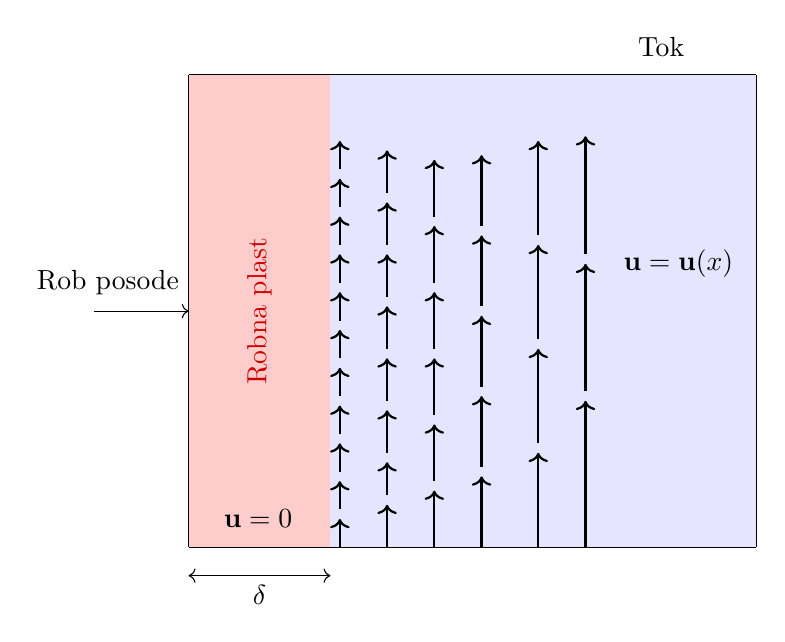
\begin{tikzpicture}[scale=1.2]

  % Draw the container walls
  \draw[thick] (0,0) -- (0,5);
  \draw[thick] (6,0) -- (6,5);
  \draw[thick] (0,5) -- (6,5);
  \draw[thick] (0,0) -- (6,0);

  % Fluid fill (optional blue fill to indicate fluid)
  \fill[blue!10] (0,0) rectangle (6,5);

  % Boundary layer shaded region
  \fill[red!20] (0,0) rectangle (1.5,5);

  % Label the boundary layer
  \node[red!80!black, rotate=90] at (0.75,2.5) {Robna plast};

  % Velocity profile (arrows)
  %\draw[->, thick] (1.5,0.5) -- (5,0.5);
  %\draw[->, thick] (1.5,2.5) -- (5.5,2.5);
  %\draw[->, thick] (1.5,4.5) -- (5,4.5);

  % Velocity labels
  \node[right] at (4.5,3) {$\bd{u} = \bd{u}(x)$};
  \node[left] at (1.2,0.3) {$\bd{u} = 0$};

  % Show arrow and label for Wall (moved to the left)
  \draw[->] (-1, 2.5) -- (0,2.5);
  \node[left] at (0,2.8) {Rob posode};

  % Delta (boundary layer thickness)
  \draw[<->] (1.5,-0.3) -- (0,-0.3);
  \node at (0.75,-0.5) {$\delta$};

  % Free stream label
  \node at (5,5.3) {Tok};

  \draw[->, thick] (1.6,0) -- (1.6,0.3);
  \draw[->, thick] (1.6,0.4) -- (1.6,0.7);
  \draw[->, thick] (1.6,0.8) -- (1.6,1.1);
  \draw[->, thick] (1.6,1.2) -- (1.6,1.5);
  \draw[->, thick] (1.6,1.6) -- (1.6,1.9);
  \draw[->, thick] (1.6,2) -- (1.6,2.3);
  \draw[->, thick] (1.6,2.4) -- (1.6,2.7);
  \draw[->, thick] (1.6,2.8) -- (1.6,3.1);
  \draw[->, thick] (1.6,3.2) -- (1.6,3.5);
  \draw[->, thick] (1.6,3.6) -- (1.6,3.9);
  \draw[->, thick] (1.6,4) -- (1.6,4.3);


  \draw[->, thick] (2.1,0) -- (2.1,0.45);
  \draw[->, thick] (2.1,0.55) -- (2.1,0.9);
  \draw[->, thick] (2.1,1) -- (2.1,1.45);
  \draw[->, thick] (2.1,1.55) -- (2.1,2);
  \draw[->, thick] (2.1,2.1) -- (2.1,2.55);
  \draw[->, thick] (2.1,2.65) -- (2.1,3.1);
  \draw[->, thick] (2.1,3.2) -- (2.1,3.65);
  \draw[->, thick] (2.1,3.75) -- (2.1,4.2);


  \draw[->, thick] (2.6,0) -- (2.6,0.6);
  \draw[->, thick] (2.6,0.7) -- (2.6,1.3);
  \draw[->, thick] (2.6,1.4) -- (2.6,2);
  \draw[->, thick] (2.6,2.1) -- (2.6,2.7);
  \draw[->, thick] (2.6,2.8) -- (2.6,3.4);
  \draw[->, thick] (2.6,3.5) -- (2.6,4.1);
  

  \draw[->, thick] (3.1,0) -- (3.1,0.75);
  \draw[->, thick] (3.1,0.85) -- (3.1,1.6);
  \draw[->, thick] (3.1,1.7) -- (3.1,2.45);
  \draw[->, thick] (3.1,2.55) -- (3.1,3.3);
  \draw[->, thick] (3.1,3.4) -- (3.1,4.15);


  \draw[->, thick] (3.7,0) -- (3.7,1);
  \draw[->, thick] (3.7,1.1) -- (3.7,2.1);
  \draw[->, thick] (3.7,2.2) -- (3.7,3.2);
  \draw[->, thick] (3.7,3.3) -- (3.7,4.3);


  \draw[->, thick] (4.2,0) -- (4.2,1.55);
  \draw[->, thick] (4.2,1.65) -- (4.2,3);
  \draw[->, thick] (4.2,3.1) -- (4.2,4.35);

\end{tikzpicture}
\caption{Posoda, kjer imamo robno plast širine $\delta$ in tokovnice $\bd{u}$, katerih hitrost se veča, bolk kot smo stran od roba.}
\end{figure}

Ponovno začnemo z Navier-Stokesovo enačbo, vendar predpostavimo, da nimamo vpliva zunanjih sil tj. $f = 0$.
$$
\frac{\partial \bd{u}}{\partial t} + (\bd{u}\cdot \nabla)\bd{u} = - \frac{1}{\rho}\nabla p + \nu \nabla^2 \bd{u}.
$$
Enačbo skalarno pomnožimo s hitrostjo $u$
\begin{align*}
\bd{u}\cdot\frac{\partial \bd{u}}{\partial t} + (\bd{u}\cdot \nabla)|\bd{u}|^2 = - \frac{1}{\rho}(\bd{u}\cdot\nabla p) + \nu (\bd{u}\cdot\nabla^2 \bd{u})
\end{align*}
Zapišimo vsak člen preko diferencialnega operatorja. Prvi in tretji člen ni težko zapisati preko gradienta:
$$
\frac{\partial}{\partial t} \Big(\frac{1}{2} \bd{|u|}^2 \Big) = \bd{u}\cdot \frac{\partial \bd{u}}{\partial t}.
$$
in
$$
\nabla \cdot (\bd{u}p) = p\underbrace{\nabla\cdot \bd{u}}_{=0} + \bd{u}\cdot (\nabla p) = \bd{u}\cdot (\nabla p)
$$
Za drugi člen, uporabimo pravilo produkta za gradient 
\begin{align*}
\nabla \cdot (|\bd{u}|^2 \bd{u}) &= \nabla(|\bd{u}|^2) \cdot \bd{u} + |\bd{u}|^2 \underbrace{(\nabla \cdot \bd{u})}_{= 0} =  (2(\bd{u}\cdot\nabla)\bd{u})\bd{u}\\[2mm]
\Longrightarrow (\bd{u}\cdot\nabla)|\bd{u}|^2 &= \nabla \cdot \Big(\frac{1}{2} |\bd{u}|^2 \bd{u}\Big).
\end{align*}

Za zadnji člen se poslužimo naslednje identitete
\begin{lema}
Naj bo $\bd{u} \in C^2$ vektorsko polje.
Velja
\begin{equation}
\bd{u}\cdot \nabla^2 \bd{u} = \nabla\cdot\Big((\bd{u}\cdot \nabla)\bd{u} - \nabla\Big(\frac{1}{2} |\bd{u}|^2\Big)\Big) - |\nabla \bd{u}|^2,
\end{equation}
kjer je 
\begin{equation}
\label{gradnorm}
  |\nabla \bd{u}|^2 = \sum_{i,j=1}^3 \Big(\frac{\partial u_i}{\partial x_j}\Big)^2.
\end{equation}
\end{lema}

Dobljeno enakost 
$$
\frac{\partial}{\partial t} \Big(\frac{1}{2} |\bd{u}|^2 \Big) + \nabla \cdot \Big(\frac{1}{2} |\bd{u}|^2 \bd{u}\Big) = 
-\frac{1}{\rho}\nabla(p \bd{u}) + \nu \nabla\cdot\Big((\bd{u}\cdot \nabla)\bd{u} - \nabla\Big(\frac{1}{2} |\bd{u}|^2\Big)\Big) - \nu|\nabla \bd{u}|^2
$$
integriramo po omejenem območju $\Omega$ z robomo $\partial \Omega$:
\begin{align*}
\int_\Omega \frac{\partial}{\partial t} \Big(\frac{1}{2} |\bd{u}|^2 \Big)\dif V + \int_\Omega \nabla \cdot\Big(\frac{1}{2} |\bd{u}|^2 \bd{u}+\frac{1}{\rho}p \bd{u} - \nu(\bd{u}\cdot \nabla)\bd{u} + \nu\nabla\Big(\frac{1}{2} |\bd{u}|^2\Big)\Big)\dif V =\int_V - \nu|\nabla \bd{u}|^2 \dif \Omega.\qquad\qquad\qquad
\end{align*}
Po izreku o divergenci:
\begin{align*}
  \int_\Omega \frac{\partial}{\partial t} \Big(\frac{1}{2} |\bd{u}|^2 \Big)\dif V + \int_{\partial\Omega} \frac{1}{2} |\bd{u}|^2 \bd{u}
  +\frac{1}{\rho}p \bd{u} - \nu(\bd{u}\cdot \nabla)\bd{u} + \nu\nabla\Big(\frac{1}{2} |\bd{u}|^2\Big)\dif \vec{S} =\int_\Omega - \nu|\nabla \bd{u}|^2 \dif V.\qquad\qquad\qquad\qquad
\end{align*}
Ker smo prevzeli robni pogoj $\bd{u}_{|_{\partial\Omega}} = 0$, srednji člen odpade in nam ostane 
$$
\int_\Omega \frac{\partial}{\partial t} \Big(\frac{1}{2} |\bd{u}|^2 \Big)\dif V = - \int_\Omega\nu|\nabla \bd{u}|^2 \dif V
$$
$$
\frac{\partial}{\partial t}\int_\Omega \frac{1}{2} |\bd{u}|^2 \dif V = - \nu\int_\Omega |\nabla \bd{u}|^2 \dif V
$$
\newpage
Kako interpretiramo dani rezultat? Levi stran enakosti nam pove, kako se kinetična energija 
v območju $\Omega$ spreminja s časom. Desni člen je negativen, saj je integrand pozitiven.
Torej kinetična energija toka s časom pada in prehaja v toploto.\\
Lahko pa povemo še malo več. Naj bo $\bd{f} \neq 0$ in ponovimo postopek. Dobimo identično enačbo, le da vsebuje še delo zunanje sile
\begin{equation}
\frac{\partial}{\partial t}\int_\Omega \frac{1}{2} |\bd{u}|^2 \dif V = - \nu\int_\Omega |\nabla \bd{u}|^2 \dif V + \int_\Omega \bd{u}\cdot \bd{f} \dif V.
\end{equation}
Če se kinetična energija s časom ne spreminja (miruje) tj. $\frac{\partial}{\partial t} |\bd{u}|^2 = 0$:
$$
 \nu\int_\Omega |\nabla \bd{u}|^2 \dif V = \int_\Omega \bd{u}\cdot \bd{f} \dif V.
$$
Ta enakost nam pove, da v primeru, ko se kinetična energija ohranja, je energija, ki odhaja iz sistema enaka energiji, ki jo dovajamo z delom telesne sile $\bd{f}$.
Ta rezultat nam da namig, da smo na pravi poti, kar se tiče analize turbulence in tokov
nasplošno, saj je rezultat ekvivalenten 1. zakonu termodinamike:
\begin{definicija}[1. zakon termodinamike]
Naj bo $\Omega$ sistem oz. omejeno območje. Potem je sprememba energije ($E$) sistema, 
enaka energiji vhodne($E_\text{in}$) in izhodne energije($E_{\text{out}}$)
\begin{equation}
\triangle E = E_\text{in} + E_{\text{out}}.
\end{equation}
\end{definicija}

\begin{definicija}
Naj bo $\bd{u}$ rešitev Navier-Stokesove enačbe in zadošča zakonu o ohranitvi mase. \textbf{Viskozna disipativnost} je 
\begin{equation}
\epsilon = \nu|\nabla \bd{u}|^2.
\end{equation}
\end{definicija}

\subsubsection{Velikostne skale}
Ključna ugotovitev v prvi polovici 20. stoletja, ki je spremenila, kako so ljudje gledali 
na turbulenco je, da se kljub njenemu kaotičnemu obnašanju, pojavijo urejene strukture. To so vrtinci. V zadnjem razdelku smo videli, da energija pada s časom, na poljubni domeni 
$\Omega$. Jasno je, če je domena večja, bo večji odtok/prenos energije. Če je turbulenten 
tok sestavljen iz vrtincev, se pojavi vprašanje, kako veliki oz. majhni so taki vrtinci? 
Ključni so vrtinci "najmanjših" velikosti zaradi naslednjega mehanizma:
energija večjega vrtinca se manjša in se prenaša na manjše vrtince. Ta postopek se ponavlja, dokler 
ne pridemo do vrtincev velikosti, pri katerih se energija ne prenese več na manjše vrtince, 
ampak se zaradi viskoznosti energija začne pretvarjati v toploto. Tem vrtincem pravimo \textbf{disipativni vrtinci}.

Še ena opazka: ko govorimo o velikih vrtincih, govorimo tudi o velikih Reynoldsovih 
številih oz. $Re >> 1$. Spomnimo se, da smo iz brezdimenzijske Navier-Stokesove enačbe 
dobili Eulerjevo enačbo \ref{Euler NS}, ki ne vsebuje viskoznega člena. To pomeni, da je 
$\nu \nabla^2 \bd{u} \approx 0$ $\Longrightarrow$ $\epsilon \approx$ konst. Zato bomo v 
nadaljevanju predpostavili, da je viskozna disipativnost konstantna (do katerih velikosti ima ta predpostavka smisel?).\\

Označimo z $\mathscr{l}$ premer poljubnega vrtinca in z $\mathscr{u}$ povprečno hitrost vrtinca.
Definiramo turbulentno Reynoldsovo število $R_t = \frac{\mathscr{u}\mathscr{l}}{\nu}$. 
V splošnem velja $Re > R_t$, vendar sta primerljiva, zato $R_t >> 1$. \\
Videli smo, kako pomembna je količina $\epsilon$, zato jo bomo povezali s količinama 
$\mathscr{l}$ in $\mathscr{u}$ preko dimenzijske analize. Enota za $\frac{\partial \bd{u}}{\partial x_i}$,
kjer je $i=1,2,3$, je $\frac{m}{s\cdot m} = \frac{1}{s}$, zato je enota za $[|\nabla \bd{u}|^2] = \frac{1}{s^2}$.
Enota za $\epsilon$ je 
\begin{align*}
[\epsilon] = \nu |\nabla \bd{u}|^2 = \frac{m^2}{s} \frac{1}{s^2} = \frac{m^2}{s^3}.
\end{align*}
Za primerno izbran čas $\tau$ dobimo oceno
\begin{equation}
\label{hitrost approx}
\epsilon \sim \frac{\mathscr{l}^2}{\tau^3} = \frac{\mathscr{u}^2}{\tau} = \frac{\mathscr{u^3}}{\mathscr{l}},
\end{equation}
kjer je $\mathscr{u} = \frac{\mathscr{l}}{\tau}$.\\
(Paradoks: zakaj je ta izraz neodvisen od $\nu$ medtem ko je definicija odvisna od $\nu$).\\
Izkaže se, da je to zelo dober način za ocenjevanje velikosti vrtincev. Velik preskok je 
naredil Andrej Nikolajevič Kolmogorov, ki je postavil hipotezo, da sta hitrost $\upsilon$ 
in dolžina $\eta$ disipativnih vrtincev odvisna le od viskozne disipativnosti $\epsilon$ 
in kinematične viskoznosti $\nu$. Poiščimo izraz zanju.
Razdalja $\eta$  se začne, ko začne prevladovati viskozni del Navier-Stokesove enačbe 
$$
\nu \nabla^2 \bd{u} > (\bd{u}\cdot \nabla)\bd{u}.
$$
Aproksimiramo vsakega posebej preko brezdimenzijske analize 
\begin{align*}
\nu \nabla^2 \bd{u} &\sim \nu \frac{\partial^2 \bd{u}}{\partial x^2} \sim \frac{\nu \mathscr{u}}{\mathscr{l}} = \frac{\nu}{\mathscr{l}\tau}. \\[2mm]
&(\bd{u}\cdot \nabla)\bd{u} \sim \frac{\mathscr{u}^2}{\mathscr{l}} \sim \frac{\mathscr{l}}{\tau}
\end{align*}
$$                                                                                                      \Longrightarrow \nu \nabla^2 \bd{u} > (\bd{u}\cdot \nabla)\bd{u} \iff \frac{\nu}{\mathscr{l}\tau} > \frac{\mathscr{l}}{\tau} \iff \mathscr{l}^2 < \nu \tau.
$$
Iz izraza \ref{hitrost approx} izpostavimo $\tau$, kar nam da:
$$
l^2 < \nu \tau = \nu \Big(\frac{\mathscr{l}^2}{\epsilon} \Big)^\frac{1}{3} \iff l < \Big(\frac{\nu^3}{\epsilon} \Big)^\frac{1}{4}.
$$
Neenakost nam da območje, kjer se začne proces disipativnosti. 
Zgornja meja hitrosti teh vrtincev:
\begin{align*}
\upsilon^3 =& \,\mathscr{l}\epsilon = \Big(\frac{\nu^3}{\epsilon}\Big)^\frac{1}{4} \epsilon = (\epsilon \nu)^\frac{3}{4} \\
&\Longrightarrow\, \upsilon = (\epsilon \nu)^\frac{1}{4}.
\end{align*}

\begin{definicija}
Naj bosta $\nu$ viskoznost in $\epsilon$ viskozna disipativnost. Definiramo Kolmogorovo hitrostno skalo 
\begin{equation}
  \upsilon = (\epsilon \nu)^\frac{1}{4}.
\end{equation}
in Kolmogorovo dolžinsko skalo 
\begin{equation}
  \eta = \Big(\frac{\nu^3}{\epsilon} \Big)^\frac{1}{4}.
\end{equation}
To sta  velikost in hitrost najmanjšega možnega vrtinca.
\end{definicija}

Poglejmo si nekaj posledic. Reynoldsovo število disipativnih vrtincev je 
$$
R_t = \frac{\upsilon\eta}{\nu} = (\epsilon \nu)^\frac{1}{4}\,\Big(\frac{\nu^3}{\epsilon} \Big)^\frac{1}{3} \,\frac{1}{\nu} = 1,
$$
kar se sklada z domnevo, da ima viskoznost velik vpliv. Poglejmo še, koliko večji in hitrejši so veliki vrtinci:
\begin{align*}
\frac{\mathscr{l}}{\eta} &= \frac{l \epsilon^\frac{1}{4}}{\nu^\frac{3}{4}} \stackrel{\ref{hitrost approx}}{\sim}
\frac{\mathscr{l} \mathscr{u}^\frac{3}{4}}{\mathscr{l}^\frac{1}{4}\nu^\frac{3}{4}} = \Big(\frac{\mathscr{u}\mathscr{l}}{\nu} \Big)^\frac{3}{4} = R_t^\frac{3}{4}, \\[1mm]
\frac{\mathscr{u}}{\upsilon} &= \frac{u}{(\epsilon \nu)^\frac{1}{4}} \stackrel{\ref{hitrost approx}}{\sim} 
\frac{\mathscr{u}}{\Big(\frac{(\mathscr{l}^3 \eta)}{\mathscr{l}}\Big)^\frac{1}{4}} = 
\Big(\frac{\mathscr{u} \mathscr{l}}{\nu}\Big)^\frac{1}{4} = R_t^\frac{1}{4}.
\end{align*}
Ker je $R_t >> 1$, nam izračun nam pove, da so disipativni vrtinci občutno manjši in 
počasnejši od energijsko bogatih vrtincev. 
\begin{primer}
Tipična hitrost in velikost vrtinca v robni plasti atmosfere sta $\mathscr{u} \sim 1 \frac{m}{s}$ in 
$l \sim 10^3$m viskoznost zraka pa je $\nu \sim 10^{-5} \frac{kg}{m s}$. Torej je 
$R_t \sim 10^8$, kar nam da oceni za hitrost in velikost disipativnih vrtincev 
$\mathscr{u} \sim 10^{-2} \frac{m}{s}$ in $\eta \sim 10^{-3}m$.
\end{primer}

Z znanjem, ki smo ga pridobili do sedaj lahko hitro pokažemo problem modeliranja turbulence
neposredno preko Navier-Stokesovih enačb. Najmanjše smiselne dolžine so velikosti $\eta$,
velikost območja, ki ga želimo modelirati, naj bo $L$. Po zgornjem razmisleku, je število potrebnih točk 
$$
N = \Big( \frac{L}{\eta} \Big) \sim R_t^\frac{3}{4}
$$
oz. v treh dimenzijah 
$$
N = \Big( \frac{L}{\eta} \Big)^3 \sim R_t^\frac{9}{4}.
$$
Iz zadnjega primera hitro postane jasno, da je modeliranje neposredno preko danih enačb 
povsem nepraktično, saj je število potrebnih točk približno $N \sim (10^8)^\frac{9}{4}
= 10^{18}$. Zato so direktne numerične simulacije uporabljajo le za manjša območja, 
na primer $R_t \sim 1000$, torej $N \sim 10^\frac{27}{4} \sim 10^7$, kar še vedno ni majhno število. 

\newpage
\section{Large eddy simulacije}

Nakoncu zadnjega poglavja smo videli, da je neposredno reševanje Navier-Stokesovih enačb 
za velike vrtince oz. tri dimenzionalno turbulentno gibanje tokov, neučinkovito. V tem poglavju 
bomo spoznali orodja, s katerimi bomo enačbe, ki opisujejo dane tokove, priredili na tak
način, da bomo lahko bolj učinkovito rešili enačba. Simulacije velikih vrtincev (eng. 
Large eddy simulations) oz. LES razdelimo na štiri korake 
\begin{enumerate}
\item[i)] Spoznali bomo koncept povprečenja in kako tok razcepimo na dva dela: 
povprečni del in spremenljivi del. Povprečni del bo predstavljal hitrostno polje 
velikih vrtincev. Osredotočili se bomo na posebno vrsto povprečja, to je filtracija.
\item[ii)] Preko filtracije Navier-Stokesovih enačb dobimo nove enačbe, ki jih bomo 
uporabili za numerično reševanje. 
\item[iii)] Zaprtje novih enačb. Pri prejšnji točki dobimo nove člene v enačbi, kar 
povzroči, da imamo več spremenljivk kot enačb. Problem bomo rešili z modeliranjem 
novih členov.
\item[iv)] Numerično rešimo zaprt sistem enačb, ki opisuje tok.
\end{enumerate}

To je najbolj splošen pristop, je pa pomembno navesti, da obstaja več podvrst LES, 
ki so odvisne od kompleksnosti in velikosti območja, ki ga obravnavamo.

\subsection{Povprečja}

Vse odvisne spremenljivke, hitrost, vrtinčnost, tlak, temperatura \dots, so turbulentne.
Intuitivno to pomeni, da so v prostoru neenakomerno porazdeljene in v vsaki točki v 
opazovanem območju kaotično oscilirajo. Zaradi naključnega obnašanja je pogosto smiselno turbulenco 
analizirati z vidika statistike. V delu se temu ne bomo posvetili, omenimo zaradi 
povprečja, ki temelji na več ponovitvah istega poskusa. \\
Ideja za povprečji je, da hitrostno polje $\bd{U}(\bd{x}, t)$ razcepimo na povprečni del $\overline{\bd{U}}(\bd{x}, t)$ in 
oscilirajoči del $\bd{u}(\bd{x}, t)$.
\begin{equation}
\bd{U}(\bd{x}, t) = \overline{\bd{U}}(\bd{x},t) + \bd{u}(\bd{x}, t).
\end{equation}
Temu razcepu pravimo Reynoldsov razcep.

Zapišimo nekaj lastnosti, ki jih želimo od povprečji. Naj bosta $\bd{U}$ in $\bd{V}$ dva tokova in 
$\alpha, \beta \in \R$:
\begin{enumerate}
  \item[i)] Linearnost: 
  $$\overline{\alpha \bd{U} + \beta \bd{V}} = \alpha \overline{\bd{U}} + \beta\overline{\bd{V}}.$$
  \item[ii)] Povprečje konstante $\bd{C}$ je $\bd{C}$:
  $$ \overline{\bd{C}} = \bd{C}.$$
  \item[iii)] Indempotentnost:
  $$ \overline{\overline{\bd{U}}} = \overline{\bd{U}}.$$
  \item[iv)] Povprečje oscilirajočega dela je $\bd{0}$:
  $$ \overline{\bd{u}} = \overline{\bd{U} - \overline{\bd{U}}} = \bd{0}.$$
  \item[v)] Pravilo produkta: 
  $$ \overline{\bd{U}\cdot \bd{V}} = \overline{\bd{U}}\cdot \overline{\bd{V}}. $$
  \item[vi)] Komutiranje z odvajanjem:
  $$ \overline{\frac{\partial \bd{U}}{\partial x_i}} = \frac{\partial \overline{\bd{U}}}{\partial x_i}.$$
\end{enumerate}

\begin{lema}
Če velja lastnost $i)$ potem je $iii) \iff iv)$
\end{lema}

\begin{proof}
\begin{align*}
\overline{\overline{\bd{U}}} = \overline{\bd{U}} \iff 0 = \overline{\bd{U}} - \overline{\overline{\bd{U}}} \stackrel{i)}{=} 
\overline{\bd{U} - \overline{\bd{U}}}.
\end{align*}
\end{proof}

\subsubsection{Ansambelsko povprečje}
Recimo, da opravljamo eksperiment in dobimo nek rezultat. Pogostokrat zaradi napak ali 
zunanjih vplivov ali majhne verjetnosti pojava željenega rezultata, poskus večkrat ponovimo in 
za naš končni rezultat vzamemo povprečje vseh rezultatov. To je ideja za ansambelskim 
povprečenjem.

Turbulenca predstavlja naša odstopanja ali šum oz. kaotičen del.
Ker se pri zelo majhnih začetnih pogojih, tok lahko zelo spremeni, nam vsaka ponovitev 
poskusa, da novo rešitev. Vsaka taka rešitev je lahko zelo drugačna od prejšnje in naslednje. 
Tem ponovitvam pravimo realizacije in označimo $\bd{U}(x, t; \alpha)$, za $\alpha \in \N$
realizacijsko število. 
\begin{definicija}
Ansambelsko povprečje toka $\bd{U}$ je 
\begin{equation}
\bd{U}^\text{avg}(\bd{x}, t) = \lim_{N\rightarrow \infty} \frac{1}{N}\sum_{\alpha=1}^N \bd{U}(\bd{x}, t;\alpha). 
\end{equation}
\end{definicija}

Bolj formalno, na $\bd{U}(\bd{x}, t;\alpha)$ gledamo kot slučajni vektor, in zaporedje 
$\bd{U}(\bd{x}, t; 1)$, $\bd{U}(\bd{x}, t; 2)$ \dots, $\bd{U}(\bd{x}, t;n)$ je zaporedje neodvisno, enako porazdeljenih 
slučajnih vektorjev. Pričakovana vrednost $E(\bd{U}_i) = \mu$ za vsak $i\in\N$, zato je po 
zakonu velikih števil, ansambelsko povprečje konvergentno.\\

Ansambelsko povprečje zadošča vsem lastnostim $i) - vi)$ zato je temelj za \\
Reynoldsovo-povprečene Navier-Stokesove simulacije (RANS). Omenimo še dve povprečji: 
\begin{definicija}
Časovno povprečje je 
\begin{equation}
\bd{U}^T(\bd{x}, t; T) = \frac{1}{T}\int_0^T \bd{U}(\bd{x}, t + \tau) \dif \tau.
\end{equation}
\end{definicija}

\begin{definicija}
Prostorsko povprečje je 
\begin{equation}
\bd{U}^T(\bd{x}, t; L) = \frac{1}{L}\int_0^L \bd{U}(\bd{x} + \bd{s}, t) \dif \bd{s}.
\end{equation}
\end{definicija}

Čeprav so ta povprečja na prvi pogled nepovazana, pa se v praksi izkaže, da imajo poseben 
pomen. Naj bo polje $\bd{U}$ stacionarno tj. $\bd{U}(\bd{x}, t) = \bd{U}(\bd{x})$ ali homogeno oz. $\bd{U}(\bd{x}, t) = \bd{U}(t)$.
Intuitivno bi pričakovali, da je 
$$
\lim_{T\rightarrow \infty} \bd{U}^T(\bd{x}, t; T) = \lim_{T\rightarrow \infty} \bd{U}^T(\bd{x}; T) = \bd{U}^\text{avg}(\bd{x})
$$
oz. 
$$
\lim_{T\rightarrow \infty} \bd{U}^S(x, t; S) = \lim_{T\rightarrow \infty} \bd{U}^S(t; T) = \bd{U}^\text{avg}(t)
$$
Če slučajna spremenljivka $\bd{U}$ oz. hitrostno polje v našem primeru, zadošča obema lastnostima, 
pravimo, da je $\bd{U}$ \textbf{ergodično}. V računski dinamiki fluidov se pogosto predpostavi, da je turbulenca ergodična. 
Temu pravimo ergodična hipoteza. Zato ne obstaja dokaz, vendar mnoge numerične simulacije in eksperimenti hipotezo potrjujejo. \\
Ergodičnost se predpostavi, saj je računanje ansambelskega povprečja težavno, ker potrebujemo 
veliko poskusov za njegov izračun, med tem, ko je prostorsko ali časovno povprečje dokaj 
enostavno.

\subsubsection{Filtracija}

Sedaj se bomo resno posvetili filtraciji, ki je posebna vrsta povprečja.
\begin{definicija}
Naj bo $\bd{U}: \R^d\times \R^+ \rightarrow \R^3$ vektorsko polje in $G: \R^d\times \R^d \rightarrow \R$.
Potem je filter polja $\bd{U}$, polje filtrirano polje $\overline{\bd{U}}$
\begin{equation}
\overline{\bd{U}}(x, t) = \int_{\R^d} G(r, x)\bd{U}(x-r, t) \dif r.
\end{equation}
Funkciji $G$ pravimo filtracijska funkcija in zadošča normalizacijskem pogoju 
$$
\int_{\R^d} G(r, x) \dif r = 1.
$$
\end{definicija}

\begin{definicija}
Naj bo $G$ filtracijska funkcija in $\bd{U}$ tok. Potem je residualno polje 
\begin{equation}
\bd{u}'(x, t) = \bd{U}(x, t) - \overline{\bd{U}(x, t)}.
\end{equation}
\end{definicija}

\begin{opomba}
  \hfill
\begin{itemize}
\item Polji $\overline{\bd{U}}$ in $u$ bomo tudi imenovali razrešen del in podfilterska skala.
\item Opazimo, da je definicija filtra skoraj identična definiciji konvolucije, le da je  
$U$ vektorsko polje in ne skalar, kot običajno.
\item Zgornji razcep je analogen Reynoldsovem razcepu, glavna razlika je, da rezidualni 
del ni nujno enak $0$
$$ \overline{\bd{u}'} \neq 0.$$
\end{itemize}
\end{opomba}

\begin{trditev}
Filtracija zadošča lasnostim $i), ii)$ in kumutarnju z časovnim odvodom. Če je filtracijska funkcija $G$ homogeno, velja lasnost $vi)$.
\end{trditev}

\begin{proof}
\begin{enumerate}
  \item[i)] Naj bosta $\bd{U}$, $\bd{V}$ vektorski polji, $\alpha, \beta \in \R$ in $G$ filtracijska 
  funkcija
  \begin{align*}
  \overline{\alpha \bd{U} + \beta \bd{V}} &= \int_{\R^d} G(r, x) (\alpha \bd{U}(x-r, t) + \beta \bd{V}(x-r, t)) \dif r = \\
  &= \int_{\R^d} \alpha G(r, x) \bd{U}(x-r, t) + \beta G(r, x) \bd{V}(x-r, t) \dif r = \\
  &= \alpha\int_{\R^d} G(r, x) \bd{U}(x-r, t)\dif r + \beta\int_{\R^d}G(r, x) \bd{V}(x-r, t) \dif r = \\
  &= \alpha \overline{\bd{U}} + \beta\overline{\bd{V}}
  \end{align*}
  \item[ii)] Naj bo $\bd{C}\in \R^3$ in $G$ filtracijska funkcija
  \begin{align*}
  \overline{\bd{C}} = \int_{\R^d} G(r, x) \bd{C} \dif r = \Big(\underbrace{\int_{\R^d} G(r, x)\dif r}_{\substack{\text{normalizacijski}\\\text{pogoj}}}\Big) \bd{C} = \bd{C}.
  \end{align*}
  \item[vi)] Naj bo $\bd{U}$ odvedljivo vektorsko polje po časovni spremenljivki in $G$ filtracijska funkcija 
  \begin{align*}
  \frac{\dif}{\dif t} \overline{\bd{U}}(x, t) &= \frac{\dif}{\dif t} \int_{\R^d} G(r, x) \bd{U}(x-r, t) \dif r = \\
  &= \mathcal{F}^{-1}\mathcal{F}\Big(\frac{\dif}{\dif t} \int_{\R^d} G(r, x) \bd{U}(x-r, t) \dif r\Big)= \\
  &= \mathcal{F}^{-1}\Big(i\omega \mathcal{F}\Big(\int_{\R^d} G(r, x) \bd{U}(x-r, t) \dif r \Big)\Big)= \\
  &= \mathcal{F}^{-1}(i\omega \hat{G}(\omega, x)\hat{\bd{U}}(x, \omega)) = \\
  &= \mathcal{F}^{-1}(\hat{G}(\omega, x) \cdot(i\omega \hat{\bd{U}}(x, \omega))) = \\
  &= \int_{\R^d} G(r, x) \frac{\dif}{\dif t} \bd{U}(x-r, t) \dif r =\\[1mm]
  &= \overline{\frac{\dif \bd{U}}{\dif t}}.
  \end{align*}

  Odvajamo še po času in predpostavimo, da lahko zamenjamo vrstni red odvajanja in integracije 
  (kateri pogoji so smiselni, da je to izpolnjejo ali si isti kot pri zgornjem izračunu?) 
  \begin{align*}
  \frac{\!\!\dif}{\dif x_i} \overline{\bd{U}}(x, t) &= \frac{\dif}{\dif x_i} \int_{\R^d} G(r, x) \bd{U}(x-r, t) \dif r = \\
  &=  \int_{\R^d} \frac{\dif}{\dif x_i} (G(r, x) \bd{U}(x-r, t)) \dif r = \\
  &=  \int_{\R^d} \frac{\dif G}{\dif x_i}(r, x)  \bd{U}(x-r, t) \dif r + \int_{\R^d} G(r, x)  \frac{\dif \bd{U}}{\dif x_i}(x-r, t) \dif r = \\
  &= \int_{\R^d} \frac{\dif G}{\dif x_i}(r, x)  \bd{U}(x-r, t) \dif r + \overline{\frac{\dif \bd{U}}{\dif x_i}}.
  \end{align*}

  $G$ je homogena torej je $G(r, x) = G(r)$, posledično 
  $$\frac{\dif G}{\dif x_i}(r, x) = \frac{\dif G}{\dif x_i}(r) = 0$$
  in enakost sledi.
\end{enumerate}
\end{proof}

\begin{opomba}
  \hfill
\begin{itemize}
  \item Ker je $\bd{U}$ vektor, integral deluje po komponentah, zato tudi Fourierova tranformacija deluje po komponentah. 
  \item V dokazu smo uporabili dejstvo 
  $$ \mathcal{F}(f')(\omega) =  i\omega \mathcal{F}(f)(\omega). $$
\end{itemize}
\end{opomba}

\noindent
Poglejmo si dva filtra, ki se pogosto uporabljata. Primera si bomo pogledali v eni dimenziji, 
kar se enostavno  posploši v višje dimenzije. Od sedaj naprej bomo predpostavili, da je 
$G$ homogeno tj. $G(r, x) = G(r)$. Matematično, je filter sedaj konvolucija, kar običajno 
zapišemo
\begin{equation}
\overline{\bd{U}}(x, t) = (\bd{U} * G)(x, t).
\end{equation}
Iz konvolucijskega izreka dobimo 
\begin{equation}
\hat{\overline{\bd{U}}} = \mathcal{F}(\overline{\bd{U}})(\xi, t) = \mathcal{F}(\bd{U})(\xi, t)\cdot \mathcal{F}(G)(\xi)= 
\hat{\bd{U}}(\xi, t)\cdot \hat{G}(\xi).
\end{equation}
\\[1mm] 

\noindent
\textbf{Valovni preklopni filter:} \\
Pokazali smo, da filter zadošča lastnostim $i), ii)$ in $vi)$. Ali lahko za pravo izbiro 
$G$ dodatno zadostimo še kateri od ostalih lastnosti? Zaradi linearnosti filtra, nam 
ostaneta le dve lastnosti: Indempotentnost in pravilo produkta. Pravilo produkta bo
zadoščeno, če bo za pravo funkcijo $G$, integral multiplikativen. Take funkcije sicer 
obstajajo, vedar so zelo raznolike in običajno nimajo fizikalnega pomena. Torej nam ostane 
le indempotentnost. Poglejmo, kako se izraža $\overline{\overline{{U}}}$ preko konvolucije:
\begin{align*}
\overline{\overline{{U}}}(x, t) &= \int_{\R} G(r) \overline{{U}}(x - r, t) \dif r = \\
&= \int_{\R} G(r) \int_{\R} G(s) {U}(x-r-s, t) \dif s \dif r = \\
&= \int_{\R} (G*{U})(x - r, t) \dif r = G*(G * {U})(x, t) \\[1mm]
&\Longrightarrow \mathcal{F}(\overline{\overline{{U}}})(\xi, t) = \mathcal{F}(G)^2(\xi)\cdot\mathcal{F}({U})(\xi, t) = \hat{G}^2(\xi) \cdot \hat{{U}}(\xi, t)
\end{align*}
Če želimo, da je $G$ indempotent
\begin{align*}
\overline{{U}} &= \overline{\overline{{U}}} \\
\hat{{U}}\hat{G} &= \hat{{U}}\hat{G}^2 \\ 
\hat{U}(\hat{G}^2 - &\hat{G}) = 0.
\end{align*}
Ker je $U \neq 0$, $G$ zavzame vrednosti $0$ in $1$. Preden si poglemo bolj specifičen primer, 
si poglejmo problem preko Fourierove vrste, kar bo pomembno pri analizi v nadaljevanju.
${U}$ razvijemo v kompleksno Fourierovo vrsto na intervalu $[0, L]$ za $L > 0$
\begin{equation}
{U}(\bd{x}, t) = \sum_{n=-\infty}^\infty a_n(t) e^{i\kappa_n x},
\end{equation}
kjer je $\kappa_n = 2\pi\frac{n}{L}$. Filtriramo ta razvoj 
\begin{align*}
\overline{U}(x, t) &= \int_{\R^d} G(r) U(x - r, t) \dif r = \\
&= \int_{\R^d} G(r) \sum_{n=-\infty}^\infty a_n(t) e^{i\kappa_n (x - r)} \dif r = \\
&= \sum_{n=-\infty}^\infty a_n(t)\Big(\int_{\R^d} G(r) e^{-i\kappa_n r}\Big) e^{i\kappa_n x}\dif r = \\
&= \sum_{n=-\infty}^\infty a_n(t) \hat{G}(\kappa_n) e^{i\kappa_n x},
\end{align*}
Kot prej je $\hat{G}$ Fourierova transformiranka funkcije $G$ 
$$
\hat{G}(\kappa) = \int_{\R^d} G(r) e^{-i\kappa r} \dif r
$$
in preko inverzne Fourierove tranformacije dobimo
$$
G(x) = \frac{1}{2\pi} \int_{\R^d} \hat{G}(\kappa) e^{i\kappa x} \dif \kappa.
$$
\begin{opomba}
V literaturi se $\hat{G}$ pogosto imenuje prenosna funkcija in se označi s $T$.
\end{opomba}

\noindent
Uporabimo filter na $\overline{U}$
\begin{align*}
\overline{\overline{U}}(x, t) &= \int_\R G(r) \overline{U}(x-r, t) \dif r = \\
&= \int_\R G(r) \sum_{n=-\infty}^\infty a_n(t) T(\kappa_n) e^{i\kappa_n (x - r)} \dif r= \\
&= \sum_{n=-\infty}^\infty a_n(t)T(\kappa_n) e^{i\kappa_n x} \int_\R G(r)e^{-i\kappa_n r} \dif r = \\
&= \sum_{n=-\infty}^\infty a_n(t)T^2(\kappa_n) e^{i\kappa_n x} \dif r
\end{align*}
Primerjamo koeficiente vrst
$$
T^2(\kappa_n) = T(\kappa_n), \quad n\in \Z
$$
kar se ujema z dosedaj ugotovljenim. Ta je izpeljava pomembna ker uvede količino 
$\kappa_n$, ki jo imenujemo $n$-to valovno število. To bo ključno za razreševanje 
polja $\overline{U}$ na diskretni množici (kar je potrebno za numerično modeliranje).
Definiramo nizko-prehodno prenosno funkcijo
$$
T_c(\kappa)=\left\{\begin{array}{l}
  1 ;\,\, |\kappa| \leq \kappa_c \\
  0 ;\,\, |\kappa| > \kappa_c
\end{array}\right.
$$
$\kappa_c \in \R$ se imenuje \textbf{preklopno valovno število}. Sedaj lahko izračunamo 
filtracijsko funkcijo $G$
\begin{align*}
G(x) &= \frac{1}{2\pi} \int_\R T_c(\kappa) e^{-i\kappa x} \dif \kappa = \\
&= \frac{1}{2\pi} \int_{-\kappa_c}^{\kappa_c} e^{-i\kappa x} \dif \kappa = \\ 
&= \frac{i}{2\pi x} e^{-i\kappa x}\Big|_{-\kappa_c}^{\kappa_c} = \\
&= \frac{i}{2\pi x} (e^{-i\kappa_c x} - e^{i\kappa_c x}) = \frac{\sin(\kappa_c x)}{\pi x}.
\end{align*} 

\begin{definicija}
Enodimenzionalni valovno preklopni filter je filter s filtracijsko funkcijo $G$
\begin{equation}
G(x) = \frac{\sin(\kappa_c x)}{\pi x}.
\end{equation}
\end{definicija}
\noindent
To lahko enostavno posplošimo na poljubno dimenzijo 
\begin{definicija}
Za $n\in \N$ definiramo $n$-dimenzionalni valovno preklopno filtracijsko 
funkcijo $G_n$
\begin{equation}
G_n(x) = \prod_{i=1}^n G(x_i) =\prod_{i=1}^n \frac{\sin(\kappa_c x_i)}{\pi x_i}.
\end{equation} 
\end{definicija}


\begin{opomba}
Lahko tudi definiramo visoko-prehodno prenosno funkcijo
$$
T_c(\kappa)=\left\{\begin{array}{l}
  1 ;\,\, |\kappa| \geq \kappa_c \\
  0 ;\,\, |\kappa| < \kappa_c,
\end{array}\right.
$$
vendar v tem filtracijska funkcija ne obstaja.
\end{opomba}


\noindent
\textbf{Škatlast filter:}\\
Nekoliko bolj naravna filtracijska funkcija, ki nas spomne prostorsko povprečje je 
škatlasta funkcija 
\begin{definicija}
Naj bodo $\Delta > 0$. Škatlasta funkcija je 
\begin{equation}
G(x)= \begin{cases}\frac{1}{\Delta} & ; x \in\left[-\frac{\Delta}{2}, \frac{\Delta}{2}\right] \\ 0 & ; \text { sicer }\end{cases}
\end{equation}
\end{definicija}

Prenosno funkcijo lahko izračunamo po zgoraj izpeljani formuli, kar nam da 
$$
T(\kappa) = \frac{\sin(\kappa \frac{\Delta}{2})}{\kappa \frac{\Delta}{2}}.
$$
Navedimo še večdimenzionalno škatlasto funkcijo
\begin{definicija}
Naj bodo $\Delta_1, \dots, \Delta_n > 0$. $n$-dimenzionalna
škatlasta funkcija je 
\begin{equation}
  G(x_1, \dots, x_n)= \begin{cases}\frac{1}{\prod_{i=1}^{n}\Delta_i} & ; x_i \in\left[-\frac{\Delta_i}{2}, \frac{\Delta_i}{2}\right] \\ 0 & ; \text { sicer }\end{cases}
\end{equation}  
\end{definicija}

\begin{opomba}
  \hfill
  \begin{itemize}
    \item Temu filtri se tudi pravi lokalno povprečje.
    \item V literaturi se občasno pojavi tudi nekoliko drugačna definicija. kjer 
    se integrira po krogli namesto po kvadratu.
  \end{itemize}
  \end{opomba}
  

\noindent
\textbf{Gaussov filter}:
Poglejmo filtracijsko funkcijo, ki se razlikuje od prejšnij dveh primerov v dveh pogledih.
Za filtracijsko funkcijo vzamemo Gaussovo funkcijo, ki za razliko od prejšnji dveh 
primeov zvezna in pomembneje pozitivna
\begin{definicija}
Naj bo $\sigma > 0$. Gaussov filter je filter dan z Gaussovo funkcijo 
\begin{equation}
G(x_1, \dots, x_n) = \frac{1}{\sqrt{2\pi}\sigma} e^{-\frac{x^2}{2\sigma^2}}.
\end{equation}
oz. $n$-dimenzionalni Gaussov filter je dan z 
\begin{equation}
G(x_1, \dots, x_n) = \frac{1}{(2\pi \sigma^2)^{n/2}} e^{-\frac{1}{2\sigma^2}(x_1^2 + \dots + x_n^2)}
\end{equation}
\end{definicija}


\subsection{Filtrirani ohranitveni zakoni}

Sedaj je čas, da uporabimo filter na enačbah, ki jih želimo numerično rešiti. V 
razdelku bomo predpostavili, da je filtracijska funkcija homogena, saj bomo potrebovali 
lastnost komutiranja filtra z odvajanjem. Do nadaljnega bomo dodatno predpostavili, 
da je $G$ poljubna, kasneje ko se bomo posvetili natančnejši analizi, jo bomo specificirali.

\subsubsection{Filtriran zakon o ohranitvi mase}

Zakon:
$$
\nabla\cdot \bd{U} = \sum_{i=1}^3 \frac{\partial \bd{U}}{\partial x_i} = \bd{0}.
$$
\noindent
Filtrirana enačba 
\begin{align*}
\overline{\nabla\cdot \bd{U}}= \overline{\sum_{i=1}^3 \frac{\partial \bd{U}}{\partial x_i}} = 
\sum_{i=1}^3 \frac{\partial \overline{\bd{U}}}{\partial x_i} = \nabla\cdot \overline{\bd{U}} = 0.
\end{align*}
\noindent
Filtriran zakon:
\begin{equation}
\nabla\cdot\overline{\bd{U}} = \bd{0}.
\end{equation}

\subsubsection{Filtriran zakon o ohranitvi gibalne količine}

Zakon: 
$$
\frac{\partial \bd{U}}{\partial t} + (\bd{U}\cdot \nabla)\bd{U} = -\frac{1}{\rho} \nabla \bd{U} + \nu\nabla^2 \bd{U} + f.
$$

\noindent
Preden enačbo filtriramo, jo bomo preoblikovali, da se znebimo nelinearnega člena ($\bd{U}\cdot \nabla)\bd{U}$.
Najprej ga razpišemo, po komponentah 
\renewcommand{\arraystretch}{2.5} % default is 1
\[
(\bd{U} \cdot \nabla) \bd{U} =
\begin{pmatrix}
U_1 \dfrac{\partial U_1}{\partial x_1} + U_2 \dfrac{\partial U_1}{\partial x_2} + U_3 \dfrac{\partial U_1}{\partial x_3} \\
U_1 \dfrac{\partial U_2}{\partial x_1} + U_2 \dfrac{\partial U_2}{\partial x_2} + U_3 \dfrac{\partial U_2}{\partial x_3} \\
U_1 \dfrac{\partial U_3}{\partial x_1} + U_2 \dfrac{\partial U_3}{\partial x_2} + U_3 \dfrac{\partial U_3}{\partial x_3}
\end{pmatrix} = \Big[\sum_{k=1}^3 U_k \frac{\partial U_j}{\partial x_k}\Big]_j
\]
in pogledamo kako se odvod produkta izraža 
$$
\sum_{k=1}^3 \frac{\partial}{\partial x_k} (U_k U_j) = \sum_{k=1}^3 \Big(U_k\frac{\partial U_j}{\partial x_k}
+ U_j\frac{\partial U_k}{\partial x_k}\Big) = (\bd{U}\cdot \nabla)\bd{U} + (\underbrace{\nabla\cdot \bd{U}}_{\substack{\text{ohranitev}\\{\text{mase}}\\=0}}) \bd{U}
= (\bd{U}\cdot \nabla)\bd{U}.
$$
Levo stran enakosti lahko bolj kompaktno zapišemo
$$
\sum_{k=1}^3 \frac{\partial}{\partial x_k} (U_k U_j) = \nabla \cdot (U_j \bd{U}) = 
\nabla \cdot [\bd{U} \bd{U}^T]_{j} = \nabla \odot [\bd{U} \bd{U}^T],
$$

kjer je $\odot$ Hadamardov produkt oz. produkt po komponentah 
\[
A \odot B = \left[ a_j \cdot b_j \right]_j.
\]
Ta zapis ni najbolj praktičen, zato bomo Navier-Stokesovo enačbo filtrerali po komponentah.
Za $j\in \{1, 2, 3\}$ imamo 
\begin{align*}
\frac{\partial U_j}{\partial t} + \nabla\cdot(U_j U) = -\frac{1}{\rho} \frac{\partial p}{\partial x_j} + \nu\nabla^2 U_j + f_j.
\end{align*}

Filtriramo enačbo, kjer upoštevamo, da filtracija komutira z odvajanjem:
\begin{align*}
  \frac{\partial \overline{U}_j}{\partial t} + \nabla\cdot(\overline{U_j U}) = -\frac{1}{\rho} \frac{\partial \overline{p}}{\partial x_j} + \nu\nabla^2 \overline{U}_j + \overline{f}_j.
\end{align*}
Enačbo lahko zapišemo še bolj kompaktno, če uporabimo Einsteinovo konvencijo 
$$
\sum_{i=1}^n a_i b_i = a_i b_i.
$$
Filtriran zakon:
\begin{equation}
\frac{\partial \overline{U}_j}{\partial t} + \frac{\partial \overline{U_i U_j}}{\partial x_i} = -\frac{1}{\rho} \frac{\partial \overline{p}}{\partial x_j} + \nu \frac{\partial^2 \overline{U}_j}{\partial x_i \partial x_i} + \overline{f}_j.
\end{equation}

\subsubsection{Filtriran zakon o ohranitvi vrtinčnosti}

Zakon:
$$
\frac{\partial \text{\bd{$\omega$}}}{\partial t} + (\bd{U}\cdot \nabla)\text{\bd{$\omega$}} = (\text{\bd{$\omega$}} \cdot \nabla)\bd{U} + \nu \nabla^2 \text{\bd{$\omega$}} + \nabla \times \bd{f}. 
$$
Podobno kot pri Navier-Stokesovih enačbah, bomo prepisali nelinearna člena v bolj primerno 
obliko
\begin{align*}
(U \cdot \nabla) \omega = \Big[\sum_{k=1}^3 U_k \frac{\partial \omega_j}{\partial x_k}\Big]_j\\
(\omega \cdot \nabla) U= \Big[\sum_{k=1}^3 \omega_k \frac{\partial U_j}{\partial x_k}\Big]_j.
\end{align*}
Fiksiramo komponento $j\in\{1, 2, 3\}$ in pogledamo odvod produkta komponent vrtinčnosti in hitrostnega polja:
\begin{align*}
\frac{\partial}{\partial x_i} (U_i \cdot\omega_j) = \sum_{i=1}^3 \frac{\partial}{\partial x_i} (U_i \cdot\omega_j) = 
\sum_{i=1}^3 \omega_j\frac{\partial U_i}{\partial x_i} + U_i\frac{\partial \omega_j}{\partial x_i} = 
\omega_j (\underbrace{\nabla \cdot \bd{U}}_{\substack{\text{ohranitev}\\\text{mase}\\=0}}) + (\bd{U}\cdot\nabla)\text{\bd{$\omega$}}
\end{align*}
\begin{align*}
\frac{\partial}{\partial x_i} (\omega_i \cdot U_j) = \sum_{i=1}^3 \frac{\partial}{\partial x_i} (\omega_i \cdot U_j) = 
\sum_{i=1}^3 U_j\frac{\partial \omega_i}{\partial x_i} + \omega_i\frac{\partial U_j}{\partial x_i} = 
U_j (\underbrace{\nabla \cdot \text{\bd{$\omega$}}}_{\substack{\text{divergenca}\\\text{rotorja}\\=0}}) + (\text{\bd{$\omega$}}\cdot\nabla)\text{\bd{U}}.
\end{align*}
Zakon zapisan v komponetnem zapisu je, pri $j\in \{1, 2, 3\}$:
\begin{equation}
\frac{\partial \omega_j}{\partial t} + \frac{\partial}{\partial x_i} (U_i \cdot \omega_j) = 
\frac{\partial}{\partial x_i} (\omega_i \cdot U_j) + \nu \nabla^2 \omega_j + \tilde{f_j}
\end{equation}
za $\tilde{f}_j = [\nabla \cdot \bd{f}]_j$.\\
Filtriran zakon:
\begin{equation}
  \frac{\partial \overline{\omega_j}}{\partial t} + \frac{\partial}{\partial x_i} \overline{U_i \cdot \omega_j} = 
  \frac{\partial}{\partial x_i} \overline{\omega_i \cdot U_j} + \nu \nabla^2 \overline{\omega_j} + \overline{\tilde{f_j}}.
\end{equation}

\subsubsection{Filtriran zakon o ohranitvi skalarja}

Zakon:
$$
\frac{\partial c}{\partial t} + \bd{U}\cdot\nabla c = \gamma \nabla^2 c.
$$
V tem primeru bo filtracija enostavna, saj lahko zaradi ohranitva mase, polje $U$ 
potegnemo znotraj gradienta in upoštevamo linearnos filtracije. \\
Filtriran zakon:
\begin{equation}
\frac{\partial \overline{c}}{\partial t} + \nabla \cdot (\overline{c\bd{U}}) = \gamma \nabla^2 \overline{c}.
\end{equation}

\subsubsection{Filtriran materialni odvod}

Izpeljane enačbe smo sicer prevedli na enačbe primernejše za modeliranje (pomen filtra bomo 
pokazali v naslednjem razdelku), vendar če, na primer, primerjamo filtrirano in 
ne filtrirano Navier-Stokesovo enačbo, sta enačbi fundementalno drugačni, saj imamo 
v drugem členu v enem primeru odvod skalarja $\overline{U_i U_j}$ v drugem pa odvod produkta 
skalarjev $U_i U_j$. Radi bi torej v filtrirani enačbi uvedli člen $\overline{U_i} \cdot \overline{U_j}$.
Vendar pa se pojavi problem, saj $\overline{U_i}\overline{U_j} - \overline{U_i U_j}$. 
\begin{definicija}
Naj bo $\bd{U}$ vektorsko polje in $\overline{\bd{U}}$ njena filtracija. Količini 
\begin{equation}
\tau_{ij}^R = \overline{U_i U_j} - \overline{U_i} \,\overline{U_j}
\end{equation}
pravimo \textbf{rezidualni napetostni tenzor}.
\end{definicija}

Iz definicije tenzorja $\tau^R$ se naravno pojavita dodatni definiciji
\begin{definicija}
Rezidualna kinetična energija je 
\begin{equation}
k_r = \frac{1}{2} \tau_{ii}^R = \frac{1}{2}\text{tr}(\tau^R).
\end{equation}
\end{definicija}

\begin{definicija}
\textbf{Izotropni rezidualni napetostni tenzor} je dan z 
\begin{equation}
\tau_{ij}^\text{izo} = \frac{2}{3} k_r \delta_{ij}
\end{equation}
\textbf{anizotropni rezidualni napetostni tenzor} pa z 
\begin{equation}
\tau_{ij}^\text{anizo} = \tau_{ij}^R - \tau_{ij}^\text{izo}.
\end{equation}
\end{definicija}

Zapišemo filtrirano Navier-Stokesovo enačbo preko teh definicij
\begin{align*}
\frac{\partial \overline{U}_j}{\partial t} + &\frac{\partial \overline{U_i U_j}}{\partial x_i} = 
\frac{\partial \overline{U}_j}{\partial t} + \frac{\partial}{\partial x_i} (\overline{U_i}\, \overline{U_j} + \tau_{ij}^R) = 
\frac{\partial \overline{U}_j}{\partial t} + \frac{\partial}{\partial x_i} \overline{U_i}\, \overline{U_j} + \frac{\partial}{\partial x_i} \tau_{ij}^R\\[2mm]
&\Longrightarrow \,\,
\frac{\partial \overline{U}_j}{\partial t} + \frac{\partial \overline{U_i}\, \overline{U_j}}{\partial x_i} = -\frac{1}{\rho} \frac{\partial \overline{p}}{\partial x_j} 
- \frac{\partial \tau_{ij}^R}{\partial x_i}+ \nu \frac{\partial^2 \overline{U}_j}{\partial x_i \partial x_i} + \overline{f}_j.
\end{align*}

Zapišemo še preko $\tau^\text{anizo}$ tenzorja:
\begin{align*}
&-\frac{1}{\rho} \frac{\partial \overline{p}}{\partial x_j} - \frac{\partial \tau_{ij}^R}{\partial x_i}+ \nu \frac{\partial^2 \overline{U}_j}{\partial x_i \partial x_i} + \overline{f}_j = \\[1mm]
&-\frac{1}{\rho} \frac{\partial \overline{p}}{\partial x_j} - \frac{\partial (\tau^\text{izo} + \tau^\text{anizo}) }{\partial x_i}+ \nu \frac{\partial^2 \overline{U}_j}{\partial x_i \partial x_i} + \overline{f}_j = \\[1mm]
&-\frac{1}{\rho} \frac{\partial (\overline{p} + \rho\tau^\text{izo})}{\partial x_j} - \frac{\partial \tau^\text{anizo} }{\partial x_i}+ \nu \frac{\partial^2 \overline{U}_j}{\partial x_i \partial x_i} + \overline{f}_j \\[2mm]
&\Longrightarrow 
\frac{\partial \overline{U}_j}{\partial t} + \frac{\partial \overline{U_i}\, \overline{U_j}}{\partial x_i} = -\frac{1}{\rho} \frac{\partial \overline{P}}{\partial x_j} 
- \frac{\partial \tau_{ij}^\text{anizo}}{\partial x_i}+ \nu \frac{\partial^2 \overline{U}_j}{\partial x_i \partial x_i} + \overline{f}_j,
\end{align*}
kjer je $\overline{P} = \overline{p} + \rho\tau^\text{izo}$ modiciran filtriran tlak 
(zakaj se ga uvede?). Iz te enačbe je jasno kako definirati filtrirani materialni odvod 
\begin{definicija}
Filtriran materialni odvod za vektorsko polje $\bd{U}$ in $\Omega \subseteq \R^n$ je preslikava 
$\frac{\overline{D}}{\overline{D}t}: C^1(\Omega) \rightarrow C^0(\Omega)$ dana s predpisom
\begin{equation}
\frac{\overline{D} \bd{V}}{\overline{D}t} = \frac{\partial \bd{V}}{\partial t} + (\overline{\bd{U}}\cdot \nabla)\bd{V}.
\end{equation}
\end{definicija}

\subsection{Razreševanje filtriranih polj}

Sedaj bomo videli, zakaj smo uvedli filtrirane enačbe, saj če 
trenutno primerjamo z nefiltriranimi enačbami nevidimo bistvene razlike.

Omejimo, se na enodomenzionalni primer polja $u$ in interval $[0, L)$, 
$L > 0$. Če polje $u$ evalviramo na $N \in \N$ točkah, nas zanima 
kolikšen mora biti velik korah $h = \frac{L}{N}$, da lahko primerno aproksimiramo 
polje $u$ in določimo željene informacije (ekvivaletno lahko fiksiramo 
korak in določamo število točk $N$)? \\
Na to uprašanje bomo odgovorili z uporabo diskretne Fourierove analize. 

\subsubsection{Diskretna Fourierova analiza}

\begin{definicija}
Naj bo $u: [a, b) \rightarrow \C$ periodična funkcija, $a < b$ in $N\in \N$. 
Diskretna Fourierova transformacija funkcije $u$ je zaporedje 
\begin{equation}
U(x(n)) = \sum_{k=0}^{N-1} u(x(k)) e^{\frac{-2\pi k n i}{N}}, \quad n = 0, 1, \dots, N-1,
\end{equation}
Inverzna diskretna Fourierova
transformacija pa je definirana kot 
\begin{equation}
  U^{-1}(x(n)) = \frac{1}{N}\sum_{k=0}^{N-1} u(x(k)) e^{\frac{2\pi k n i}{N}}, \quad n = 0, 1, \dots, N-1.
\end{equation}
V obeh primerih je $x(k) = a + \frac{k}{N}(b-a)$, kar bomo označili kot
$x_k = x(k)$.
\end{definicija}

\begin{opomba}
Če funkcijo $u$ iz definicije trasliramo, je dovolj če se 
omejimo na interval $[0, L]$. V tem primeru je $x(k) = \frac{kL}{N}$.
\end{opomba}

Pričakovali bi, da imata diskretni Fourierovi transformaciji podobne 
lastnosti kot klasična Fourierova transformacija, kar povemo z naslednjim izrekom 

\begin{izrek}
\label{izrek:iDFT}
Naj bo $u: [a, b) \rightarrow \C$ periodična funkcija in $N\in \N$. Potem velja
\begin{equation}
U^{-1}(U(x_n)) = u(x_n) = U(U^{-1}(x_n)).
\end{equation}
\end{izrek}

\begin{dokaz}
\begin{align*}
  U^{-1}(U(x_n)) &= \frac{1}{N}\sum_{k=0}^{N-1} U(x_k) e^{\frac{2\pi k n i}{N}} = \\
  &= \frac{1}{N}\sum_{k=0}^{N-1} \sum_{j=0}^{N-1} u(x_j) e^{\frac{-2\pi i j k}{N}} e^{\frac{2\pi i k n }{N}} = \\
  &= \frac{1}{N}\sum_{k=0}^{N-1} \sum_{j=0}^{N-1} u(x_j) e^{\frac{-2\pi i k(n - j)}{N}} = 
\end{align*}

Označimo $x = e^{\frac{2\pi i (n-j)}{N}}$ in zamenjamo vrstni red seštevanja v 
zadnji enakosti 
\begin{align*}
=& \frac{1}{N}\sum_{j=0}^{N-1} u(x_j)\sum_{k=0}^{N-1} x^k .
\end{align*}
Notranja vsota je geometrijska vsota in je enaka

\[ 
  \sum_{k=0}^{N-1} x^k = \begin{cases} 
      \frac{x^N - 1}{x - 1} &; x\neq 1 \\
      \,\,\,N &; x = 1 
   \end{cases}
\]
Ker je $n-j \in \Z$, je $x^N = e^{2\pi i(n-j)} = 1$, zato lahko dodatno
poenostavimo  
\[ 
  \sum_{k=0}^{N-1} x^k = \begin{cases} 
      \,\,\,0 &; x\neq 1 \\
      \,\,\,N &; x = 1 
   \end{cases}
   = 
   \begin{cases} 
    \,\,\,0 &; j\neq n \\
    \,\,\,N &; j=n 
 \end{cases}
 = N\delta_{jn}
\]
\begin{align*}
  =& \frac{1}{N}\sum_{j=0}^{N-1} u(x_j)\sum_{k=0}^{N-1} x^k = \sum_{j=0}^{N-1} u(x_j) \delta_{jn} = u(x_n). 
\end{align*}
Enak način dokažemo tudi drugo enakost.
\end{dokaz}

Poglejmo si še nekaj pomebnih lasnotsti diskretne Fourierove transformacije
\begin{trditev}
Naj bo $u: [a, b) \rightarrow \C$ periodična funkcija, $N\in \N$ in\quad
$t, n \in \{0, 1, \dots, N-1\}$. Potem veljajo naslednje lastnosti:
\begin{enumerate}
  \item[i)] Periodičnost:
  \begin{equation}
    U(x_n) = U(x_{n + N}).
  \end{equation}
  \item[ii)] Invarianca za translacijo indeksa:
  \begin{equation}
  \sum_{k=t}^{N-1 + t} u(x_k) e^{\frac{-2\pi i k n}{N}} = \sum_{k=0}^{N-1} u(x_k) e^{\frac{-2\pi i k n}{N}}.
\end{equation}
  \item[iii)] Prostorski premik: tranformiranka funkcije $u(x - t)$ je
  \begin{equation}
  U^s(x_n) = U(x_n)e^{\frac{-2\pi k m t}{N}} .
\end{equation}
  \item[iv)] Konjugacijska simetrija: 
  \begin{equation}
    \overline{U(x_n)} = U(x_{N-n}).
  \end{equation}
  \item[v)] Plancherel izrek:
  \begin{equation}
    \sum_{k=0}^{N-1} |u(x_k)|^2 = \frac{1}{N}\sum_{n=0}^{N-1} |U(x_k)|^2.
  \end{equation}
\end{enumerate}
\end{trditev}

\begin{dokaz}
  \hfill
\begin{enumerate}
  \item[i)]
  \begin{align*}
    U(x_{n+N}) &= \sum_{k=0}^{N-1} u(x_{k+N}) e^{\frac{-2\pi k i(n+N)}{N}} = \\
    &= \sum_{k=0}^{N-1} u(x_k) e^{\frac{-2\pi k n i}{N}} e^{-2\pi k i} = \\
    &= \sum_{k=0}^{N-1} u(x_k) e^{\frac{-2\pi k n i}{N}} = U(x_n).
  \end{align*}
\newpage
  \item[ii)]
  \begin{align*}
    &\sum_{k=t}^{N-1 + t} u(x_k) e^{\frac{-2\pi i k n}{N}} = \sum_{k=0}^{N-1} u(x_{k+t}) e^{\frac{-2\pi i (k+t) n}{N}} = \\
    =&\sum_{k=0}^{N-t-1} u(x_{k+t}) e^{\frac{-2\pi i (k+t) n}{N}} + 
    \sum_{k=N-t}^{N-1} u(x_{k+t}) e^{\frac{-2\pi i (k+t) n}{N}} = 
  \end{align*}
Obravnavamo vsako vsoto posebaj: 
\begin{align*}
\sum_{k=0}^{N-t-1} u(x_{k+t}) e^{\frac{-2\pi i (k+t) n}{N}} &= 
\sum_{k=t}^{N-1} u(x_{k}) e^{\frac{-2\pi i k n}{N}}\\[5mm]
  \sum_{k=N-t}^{N-1} u(x_{k+t}) e^{\frac{-2\pi i (k+t) n}{N}} &= 
  \sum_{k=-t}^{-1} u(x_{N+k+t}) e^{\frac{-2\pi i (k+t+N) n}{N}} = \\
  &= \sum_{k=-t}^{-1} u(x_{k+t}) e^{\frac{-2\pi i (k+t) n}{N}} \\
  &= \sum_{k=0}^{t-1} u(x_{k}) e^{\frac{-2\pi i k n}{N}}
\end{align*}
končna vsota je 
$$
= \sum_{k=t}^{N-1} u(x_{k}) e^{\frac{-2\pi i k n}{N}} + \sum_{k=0}^{t-1} u(x_{k}) e^{\frac{-2\pi i k n}{N}} = 
\sum_{k=0}^{N-1} u(x_{k}) e^{\frac{-2\pi i k n}{N}}
$$

\item[iii)] 
Označimo tranformiranko od $u(x-t)$ s $U^s$. Potem je 
  \begin{align*}
    U^s(x_{n}) &= \sum_{k=0}^{N-1} u(x_{k-t}) e^{\frac{-2k \pi i n}{N}} = \\
    &= \sum_{k=-t}^{N-1-t} u(x_{k}) e^{\frac{-2(k+t) \pi i n}{N}} = \\
    &= e^{\frac{-2\pi i t n}{N}} \sum_{k=-t}^{N-1-t} u(x_{k}) e^{\frac{-2k \pi i n}{N}} \stackrel{ii)}{=} \\
    &=e^{\frac{-2\pi i t n}{N}} \sum_{k=0}^{N-1} u(x_{k}) e^{\frac{-2k \pi i n}{N}} \stackrel{ii)}{=} \\
    &= e^{\frac{-2\pi i t n}{N}} U(x_n).
  \end{align*}

\item[iv)]
\begin{align*}
  \overline{U(x_n)} = \overline{\sum_{k=0}^{N-1} u(x_k) e^{\frac{-2\pi i k n}{N}}} &= 
  \sum_{k=0}^{N-1} u(x_k) \overline{e^{\frac{-2\pi i k n}{N}}}=\\
  &= \sum_{k=0}^{N-1} u(x_k) e^{\frac{2\pi i k n}{N}}=  \\
  &= \sum_{k=0}^{N-1} u(x_k) e^{-\frac{2\pi i (N-k) n}{N}}= \\
  &= U(x_{N-n}).
\end{align*}
\item[v)] 
\begin{align*}
|U(x_n)|^2 &= U(x_n) \overline{U(x_n)} = \\
&= \sum_{k=0}^{N-1} u(x_k) e^{\frac{-2\pi i k n}{N}} \sum_{j=0}^{N-1} \overline{u(x_j)} e^{\frac{2\pi i j n}{N}} = \\
&= \sum_{k=0}^{N-1} \sum_{j=0}^{N-1} u(x_k) \overline{u(x_j)} e^{\frac{-2\pi i (k-j) n}{N}} = 
\end{align*}
\begin{align*}
\Longrightarrow \sum_{n=0}^{N-1} |U(x_n)|^2 &= \sum_{n=0}^{N-1} \sum_{k=0}^{N-1} \sum_{j=0}^{N-1} u(x_k) \overline{u(x_j)} e^{\frac{-2\pi i (k-j) n}{N}} = \\
&= \sum_{k=0}^{N-1}u(x_k) \sum_{j=0}^{N-1} \overline{u(x_j)} \sum_{n=0}^{N-1} e^{\frac{-2\pi i (k-j) n}{N}} = \\
\end{align*}

Kot pri dokazu izreka \refeq{izrek:iDFT} zapišemo 
\begin{align*}
\sum_{n=0}^{N-1} e^{\frac{-2\pi i (k-j) n}{N}} = N \delta_{kj}.
\end{align*}

Dokaz sedaj hitro sledi 
\begin{align*}
&= \sum_{k=0}^{N-1}u(x_k) \sum_{j=0}^{N-1} \overline{u(x_j)} \sum_{n=0}^{N-1} e^{\frac{-2\pi i (k-j) n}{N}} = \\
&= N\sum_{k=0}^{N-1} \sum_{j=0}^{N-1} u(x_k)\overline{u(x_j)} \delta_{kj} = \\
&= N\sum_{k=0}^{N-1} |u(x_k)|^2.
\end{align*}
\end{enumerate}
\end{dokaz}

Poglejmo sedaj si poglejmo nekaj posledic dokazanih lastnosti in malo 
širšo sliko našega cilja. \\

Očitna ampak močna posledica izreka \ref{izrek:iDFT} je, da lahko 
vrednost funkcije zapišemo kot končno vsoto eksponentnih funkcij 
\begin{equation}
  \label{eq:DFT decomposition}
u(x_n) = \sum_{k=0}^{N-1} a_k e^{\frac{2\pi i k n}{N}},
\end{equation}
kjer so koeficienti $a_k$ diskretne Fourierove transformiranke 
\begin{equation}
a_k = \frac{1}{N} U(x_k) = \frac{1}{N} \sum_{j=0}^{N-1} u(x_j) e^{\frac{-2\pi i j k}{N}}.
\end{equation}
Iz definije DFT (diskretne Fourierove transformacije) se spomnimo, da je 
argument $x_k = \frac{k L}{N}$, kjer je $L$ dolžina intervala. Zapišimo 
razvoj \ref{eq:DFT decomposition} preko tega argumenta 
$$
e^{\frac{-2\pi i k n}{N}} = e^{\frac{-2\pi k}{L}\frac{nL}{N}i} = e^{i\kappa_k x_n}
$$
torej je 
\begin{equation}
u(x_n) = \sum_{k=0}^{N-1} a_k e^{i\kappa_k x_n},
\end{equation}
kjer je $\kappa_k = \frac{2\pi k}{L}$ valovna število ali frekvenca.
To število smo že srečali, ko smo govorili o valovnem preklopnem 
filtru, ki se bo pokazalo, da je ključno pri velikosti koraka $h$ 
za numerično reševanje filtriranih enačb. Še zadnjno spremembo, ki 
jo opravimo je, da zamaknemo vrsto, da bo (čim bolj) simetrična okoli ničle. 
Po lastnosti $iii)$ lahko zamaknemo indeks seštevanja $k$ za $N/2 - 1$, pri 
predpostavki, da je $N$ sodo število
\begin{equation}
  \label{eq:DFS expantion}
u(x_n) = \sum_{k=1-\frac{N}{2}}^{\frac{N}{2}} a_k e^{i\kappa_k x_n}.
\end{equation} 

V praksi se DFS uporablja, ker Fourierovo transformacijo in 
Fourierovo vrsto le redko kdaj lahko izračunamo analitično.
Izkaže se, da pri obravnavanih lahko to naredimo točno 
\begin{izrek}
Naj bo $u: [0, L] \rightarrow \R$ periodična funkcija s periodo $N\in \N$, katere Fourierov 
razvoj obstaja. Potem je 
\begin{equation}
u(x_n) = \sum_{k=1-\frac{N}{2}}^{\frac{N}{2}} a_k e^{i\kappa_k x_n} =
\sum_{k=-\infty}^{\infty} b_k e^{i\kappa_k x_n},
\end{equation}
zveza med koeficienti $a_k$ in $b_k$ je
\begin{equation}
  a_k = \sum_{m=-\infty}^{\infty} b_{k + mN}. 
\end{equation}
\end{izrek}

\begin{dokaz}
Razvijemo vrednost $u(x_n)$ v Fourierovo vrsto 
$$
u(x_n) = \sum_{k=-\infty}^{\infty} b_k e^{i\kappa_k x_n}
$$
in ločimo na dva primera: \\
\begin{enumerate}
  \item[i)] Naj bo $b_k = 0$ za $|\kappa_k| \geq \kappa_{\text{max}}$, kjer je 
  $\omega_{\text{max}} = \omega_{N/2}$. Potem je vsota indeksirana od 
  $-(\frac{1}{2} - 1)$ do $\frac{1}{2}N - 1$
  $$
  u(x_n) = \sum_{k=1-\frac{N}{2}}^{\frac{N}{2}-1} b_k e^{i\kappa_k x_n}
  $$
  in je očitno, da so $b_k = c_k$. 
  \item[ii)] Poglejmo si sedaj splošen primer, brez omejitve na koeficiente 
  $c_k$. Naj bo $k \in \{-(\frac{1}{2}N - 1), \dots (\frac{1}{2}N - 1)\}$. 
  Po osnovnem izreku o deljenju, poljuben indeks zapišemo kot
  $k + mN$ za $m\in \Z$. Valovno število za ta indeks je 
  $$
  \kappa_{k + mN} = \frac{2\pi (k + mN)}{L} = \frac{2\pi k}{L} + 2m\frac{2\pi \frac{N}{2}}{L} = \kappa_k + 2m \kappa_{\text{max}}
  $$
  Eksponenti se poenostavijo 
  $$
  e^{i \kappa_{k + mN} x_n} =  e^{i \kappa_{k} x_n}  e^{2mi\kappa_{\text{max}} x_n} = 
  e^{i\kappa_k x_m} e^{2\pi i k m} = e^{i\kappa_k x_m}
  $$
  Potem se Fourierova vrsta zreducira na 
  \begin{align*}
  u(x_n) &= \sum_{k=-\infty}^{\infty} b_k e^{i\kappa_k x_n} = \\
         &= \sum_{m=-\infty}^{\infty} \Big(\sum_{k=1-\frac{N}{2}}^{\frac{N}{2}-1} b_{k+mN} e^{i\kappa_{k+mN} x_n}\Big) =\\ 
         &= \sum_{m=-\infty}^{\infty} \Big(\sum_{k=1-\frac{N}{2}}^{\frac{N}{2}-1} b_{k+mN} e^{i\kappa_{k} x_n}\Big) =\\ 
         &= \sum_{k=1-\frac{N}{2}}^{\frac{N}{2}-1} e^{i\kappa_{k} x_n}\Big(\sum_{m=-\infty}^{\infty} b_{k+mN}\Big) =\\
         &= \sum_{k=1-\frac{N}{2}}^{\frac{N}{2}-1} a_k e^{i\kappa_{k} x_n},
\end{align*}
kjer so koeficienti $a_k$ enaki 
$$a_k = \sum_{m=-\infty}^{\infty} b_{k+mN}.$$
\end{enumerate}
\end{dokaz}

Ta rezultat pomeni, da lahko Fourierovo vrsto, ki je v splošnem nemoremo 
točno izračunati, v tem primeru točno prevedemo na končno vsoto preko 
diskretne Fourierove transformacije. \\

\noindent
Naj bo hitrostno polje $u: \R \rightarrow \R$ periodično z periodo $L$.
Potem lahko $u$ razvijemo kot v \refeq{eq:DFS expantion}:
$$
u(x) = \sum_{k=1-\frac{N_{\text{max}}}{2}}^{\frac{N_\text{max}}{2}} a_k e^{i\kappa_k x}.
$$
za nek $N \in 2\N$, $a_k \in \C$ in $\kappa_k = \frac{2\pi k}{L}$. 
Za funkcijo $u$ torej potrebujemo vsaj $N_{\text{max}}$ vrednosti, ločene s korakom $h_{\text{max}}$,
$u(n h_{\text{max}})$, $n = 0, 1, 2, \dots, N - 1$, da jo točno predstavimo.
Na začetku razdelk smo videli, da je korak $h_\text{max}$ dan z 
$$
h_\text{max} = \frac{L}{N_\text{max}}.
$$
To prevedemo na maksimalno valovno število, ki je pojavi v DFS razvoju 
$$
h_\text{max} = \frac{L}{N_\text{max}} = \frac{\pi L}{L \kappa_{{N_\text{max}/2}}} = \frac{\pi}{\kappa_{N_\text{max}/2}}.
$$

Ker delamo s filtriranimi polji, poglejmo še Fourierovo vrsto filtriranega polja:
\begin{equation}
\label{eq:filterDFT}
\overline{u}(x) = \sum_{k=1-\frac{N_{\text{max}}}{2}}^{\frac{N_\text{max}}{2}} \overline{a}_k e^{i\kappa_k x}.
\end{equation}
Da poišemo zvezo med koeficienti $a_n$ in $\overline{a}_n$, filtriramo polje $u$
\begin{align*}
\overline{u}(x) &= \overline{\sum_{k=1-\frac{N_{\text{max}}}{2}}^{\frac{N_\text{max}}{2}} a_k e^{i\kappa_k x}} = \\
&= \sum_{k=1-\frac{N_{\text{max}}}{2}}^{\frac{N_\text{max}}{2}} a_k \overline{e^{i\kappa_k x}} = \\ 
&= \sum_{k=1-\frac{N_{\text{max}}}{2}}^{\frac{N_\text{max}}{2}} a_k \int_{\R^n} G(r)\cdot e^{i\kappa_k(x - r)} \dif r = \\
&= \sum_{k=1-\frac{N_{\text{max}}}{2}}^{\frac{N_\text{max}}{2}} a_k e^{i\kappa_n x }\int_{\R^n} G(r)\cdot e^{-i\kappa_k r} \dif r =\\
&= \sum_{k=1-\frac{N_{\text{max}}}{2}}^{\frac{N_\text{max}}{2}} a_k \hat{G}(\kappa_n) e^{i\kappa_k x}
\end{align*}
kjer je $\hat{G}$ Fourierova transformiranka filtracijske funkcije $G$. Zveza med koeficienti je torej 
\begin{equation}
  \label{koef_filter}
\overline{a}_k = \hat{G}(\kappa_k) a_k = T(\kappa_k) a_k.
\end{equation}

Sedaj lahko uporabimo izpeljano teorijo, da določimo velikost koraka $h$ 
za konkretne filtre v eni dimenziji. 

\begin{opomba}
Nauk razdelka, je da lahko polje $u$ točno predstavimo, z končnim naborom 
vrednosti oz. od neke točke naprej, ne bo dobili nič boljši rezultat, če 
uporabimo več funkcijskih vrednosti.
\end{opomba}

\subsubsection{Valovno preklopni filter}

Spomnimo se, da je valovno preklopni filter je dan z prenosno funkcijo 

$$
T_c(\kappa)=\begin{cases}
  1 ;\,\, |\kappa| \leq \kappa_c \\
  0 ;\,\, |\kappa| > \kappa_c
\end{cases}
$$
za $\kappa_c < \kappa_\text{max} = \kappa_{N_\text{max}/2}$. $\kappa_c$
izberemo tako, da je 
$$
N = \frac{\kappa_c L}{\pi} \in 2\N.
$$
Koeficienti $\overline{a_k}$ so enaki 
$$
\overline{a}_k=\begin{cases}
  a_k ;\,\, |\kappa_k| \leq \kappa_c \\
  0 \,\,;\,\,\, |\kappa_k| > \kappa_c
\end{cases}
$$
Zapišemo pogoje preko vrednosti $N$
\begin{align*}
|\kappa_k| = \Big| \frac{2\pi k}{L} \Big| &\leq \kappa_c = \frac{N\pi}{L} \Longrightarrow\\[1mm]
|k| &\leq \frac{N}{2}
\end{align*}
Torej je

$$
\overline{a}_k= \begin{cases}a_k ;\,\, |k| \leq \frac{N}{2} \\ 0 \,\,;\,\, |k| > \frac{N}{2}\end{cases}
$$
in Fourierova vrsta filtriranega polja 
\begin{equation}
\label{Fourier_število}
\overline{u}(x) = \sum_{k = 1 - \frac{1}{2}N}^{\frac{1}{2}N} a_n e^{i\kappa x}.
\end{equation}

Brez izgube informacij, lahko vrednosti $\overline{u}(nh)$ predstavimo na mreži 
z razmikom 
\begin{equation}
h = \frac{L}{N} = \frac{\pi}{\kappa_c}.
\end{equation}
Tej dolžini pravimo \textbf{karakteristična filterska dolžina} in jo 
označimo z $\Delta$. 
\noindent
Sedaj se prvič vidi bistvo filtracije. Vemo, da za neko število 
$N\in \N$, lahko $u$ točno predstavimo, vendar je to pogosto neučinkovito, 
saj, prostorska in časovna zahtevnost zelo hitro rasteta. Če pa izberemo
$\kappa_c$ primerno majhen, se število členov v vsoti zmanjša.
Sicer rešitev zgubi natančnost, vendar pa pridobimo na učinkovitosti reševanja. 
Kako izbrati mejo (v tem primeru $\kappa_c$) t.j. kako natačno želimo, 
da naša rešitev je in koliko pridobimo na učinkovitosti, bo tema naslednjega poglavja.

\subsubsection{Gaussov filter}

Sedaj bomo obravnavali Gaussov filter. Uporabimo razvoj \ref{eq:filterDFT}
$$
\overline{u}(x) = \sum_{k=1 - \frac{N_{\text{max}}}{2}}^\frac{N_{\text{max}}}{2} \overline{a}_k e^{i\kappa_k x}
$$
in poiščimo koeficiente $\overline{a}_k$, v odvisnosti od $a_k$.
\begin{align*}
T(\kappa_k) &= \int_\R G(r) \cdot e^{-i\kappa_k r} \dif r = \\
            &=\int_\R \frac{1}{\sqrt{2\pi \sigma^2}} e^{-\frac{r^2}{2\sigma^2}} \cdot e^{-i\kappa_k r} \dif r = \\
            &= \frac{1}{\sqrt{2\pi \sigma^2}} \int_\R e^{-\frac{r^2}{2\sigma^2} - i\kappa_k r} \dif r = 
\end{align*}
Dopolnimo izraz $-\frac{r^2}{2\sigma^2} - i\kappa_k r$ do popolnega kvadrata
\begin{align*}
-\frac{r^2}{2\sigma^2} - i\kappa_k r &= - \frac{1}{2\sigma^2}(r^2 + 2\sigma^2 i \kappa_k) = \\
&=-\frac{1}{2\sigma^2} ((r + i\sigma^2 \kappa_k)^2  + \sigma^4 \kappa_k^2) = \\
&=- \left(\frac{r + i\sigma^2 \kappa_k}{\sigma\sqrt{2}}\right)^2 - \frac{1}{2} \sigma^2 \kappa_k^2.
\end{align*}
Integral postane 
\begin{align*}
  =& \frac{1}{\sqrt{2\pi \sigma^2}} \int_\R e^{-\left(\frac{r + i\sigma^2 \kappa_k}{\sigma\sqrt{2}}\right)^2 - \frac{1}{2} \sigma^2 \kappa_k^2} \dif r = \\
  =& \frac{1}{\sqrt{2\pi \sigma^2}} e^{ - \frac{1}{2} \sigma^2 \kappa_k^2} \int_\R e^{-\left(\frac{r + i\sigma \kappa_k}{\sqrt{2}}\right)^2} \dif r = \\[2mm]
  &\text{ uvedemo }\,\, x = \frac{r + i\sigma^2 \kappa_k}{\sigma\sqrt{2}} \Longrightarrow \dif x = \frac{1}{\sigma\sqrt{2}} \dif r \\[2mm]
  =& \frac{1}{\sqrt{\pi}} e^{- \frac{1}{2} \sigma^2 \kappa_k^2} \int_\R e^{-x^2} \dif r = e^{- \frac{1}{2} \sigma^2 \kappa_k^2}
\end{align*}
Upoštevamo definicijo $\kappa_k = \frac{2\pi k}{L}$, so potem koeficienti $\overline{c}_k$
\begin{equation}
  \overline{a}_k = e^{-\frac{2\pi^2 \sigma^2 k^2}{L^2}} a_k.
\end{equation}
Naj bo $N < N_\text{max}$ in poglejmo aproksimacijo
\begin{equation}
\overline{u}(x) \approx \tilde{u}(x) = \sum_{k=1 - \frac{N}{2}}^\frac{N}{2} \tilde{a}_k e^{i\kappa_k x},
\end{equation}
kjer je največje valovno število $\kappa_r = \kappa_{N/2} = \frac{\pi}{h}$. Razmerje valovnih števil,
nam da 
$$
\frac{\kappa_c}{\kappa_r} = \frac{\frac{\pi}{\Delta}}{\frac{\pi}{h}} = \frac{h}{\Delta}.
$$
Koliko moramo skrajšati vrsto $\tilde{u}$, oz. kakšno razmerje $\frac{h}{\Delta}$ izbrati, da 
dobimo dobro aproksimacijo in kaj sploh pomeni, dobra aproksimacija 
odgovorimo v naslednjem poglavju. 

\subsubsection{Škatlast filter}
Poglejmo si še zadnji filter, ki smo ga omenili, to je 
škatlast filter, za katerega prenosno funkcijo že poznamo. t.j.
$$
T(\kappa) = \frac{\sin(\kappa \frac{\Delta}{2})}{\kappa \frac{\Delta}{2}}
$$
koeficineti filtriranega polja izraženi preko teh pa so 
$$
\overline{a}_k = \frac{\sin(\kappa_k \frac{\Delta}{2})}{\kappa_k \frac{\Delta}{2}} a_k = \frac{\sin(k\pi\frac{\Delta}{L})}{\pi k\frac{\Delta}{L}} a_k .
$$


\section{Energija in spektralna analiza}

V tem poglavju bomo turbulenten tok obravnavali z vidika statiske, 
vendar se bomo hitro začeli nanašati na Fourierovo analizo, ki 
se je v prejšnjem poglavju pokazala za zelo uporabno. Ta način 
modeliranja turbulence je prvi razvil Kolmogorov, ideja za tak 
opis pa predvsem pride iz kaotičnosti turbulence. Iz tega razloga se 
privzame, da je hitrostno polje $u$ slučajno. To pomeni, da 

\subsection{Osnovni pojmi}

Spomnimo se nekaj osnovnih pojmov

\begin{definicija}
Trojici $(\Omega, \mathcal{F}, P)$ pravimo \textbf{verjetnostni prostor}, 
kjer so $\Omega$ vzorčni prostor, $\mathcal{F}$ sigma algebra in 
$P$ verjetnostna mera. Preslikava $x: \Omega \rightarrow [0, 1]$ 
je \textbf{slučajna spremenljivka}, če je je merljiva. 
\textbf{Slučajni vektor} je preslikava $X: \Omega \rightarrow [0, 1]^n$, 
za $n\in \N$, kjer so komponente $X_i$ slučajne spremenljivke.
\end{definicija}

Mi se bomo omejili na primer, ko je $\Omega = \R^4$, $\mathcal{F}$ 
Lebesguevova sigma algebra, verjetnostna mera $P$ pa ni znana. 
Dodatno bomo predpostavili, da imamo slučajnost le v prostorskih 
spremenljivkah, času pa naj bo za tok determinističen. 

\begin{definicija}
Naj bo $\bd{U}$ slučajni vektor na verjetnostnem prostoru $(\Omega, \mathcal{F}, P)$,
kjer je $\Omega \subseteq \R^n$, $\mathcal{F} \in \mathcal{P}(\R)$ in $P$ probabilistična mera.
Kumulativna porazdelitve funkcija je
\begin{equation}
F_\bd{U}(V; x, t) = P(U_1(x, t) < V_1, \dots, U_n(x, t) < V_n)
\end{equation}
za $i = 1, \dots, n$ in $V \in \Omega$. Porazdelitvena 
gostota pa je 
\begin{equation}
f_U(V; x, t) = \frac{\partial^n F}{\partial x_1 \dots \partial x_n}(x, t)
\end{equation}
\end{definicija}

\begin{opomba}
Predpostavimo, da je probabilistična mera $P$ dovolj gladka, da je definicija dobra.
\end{opomba}

\begin{definicija}
Naj bo $\bd{U}$ slučajni vektor. Srednja (pričakovana) vrednost je 
\begin{equation}
\langle \bd{U}(x, t) \rangle = \int_{\R^n} V \cdot f(V; x, t) \dif V.
\end{equation}
\end{definicija}

\begin{definicija}
Naj bosta $\bd{U}$ in $\bd{V}$ slučajna vektorja. Kovarianca je 
\begin{equation}
\text{cov}(\bd{U}, \bd{V}) = \langle (\bd{U} - \langle \bd{U} \rangle)\cdot (\bd{V} - \langle \bd{V} \rangle)^T \rangle
\end{equation}
\end{definicija}

\begin{opomba}
Enakost iz prejšnje definicije z malo računanja lahko prepišemo v 
\begin{equation}
\text{cov}(\bd{U}, \bd{V}) = \langle \bd{U}\cdot \bd{V}^T \rangle - \langle \bd{U} \rangle  \langle \bd{V} \rangle^T
\end{equation}
\end{opomba}

\noindent
$F$ oz. $f$ nepoznamo. V praksi ali teoriji se pogosto se definira različna vrsta povprečja, 
ki jih je ali lažje obravnavati (prostorsko povprečje) ali lažje izračunati(ensambelsko povprečje).
V določenih scenarij približna povprečja konvergirajo k pravemu 
ali celo konvergirajo ena k drugem (ergodična hipoteza). 

\begin{definicija}
Naj bo $\bd{U}: \R^n \times \R^+ \rightarrow \C^m$ periodična v prvi spremenljivki za $L>0$ t.j. 
$$
\forall N\in \Z^n: \,\bd{U}(\bd{x} + L\bd{N}, t) = \bd{U}(\bd{x}, t).
$$
Kompleksna Fourierova vrsta preslikave $\bd{U}$ je 
\begin{equation}
\bd{U}(\bd{x}, t) = \sum_{\bd{k}\in \Z^{n}} \hat{\bd{u}}(\bd{\text{$\kappa$}}_\bd{k}, t) e^{i\bd{\text{$\kappa$}}_\bd{k} \cdot \bd{x}},
\end{equation}
$\bd{\text{$\kappa$}}_\bd{k} = \frac{2\pi}{L} \bd{k}$ in koeficienti $\hat{\bd{u}}_\bd{k}$ dani z 
\begin{equation}
\hat{\bd{u}}(\bd{\text{$\kappa$}}_\bd{k}, t) = \frac{1}{L^n} \int_{[0, L]^n} \bd{U}(\bd{x}, t) e^{-i\bd{\text{$\kappa$}}_\bd{k} \cdot \bd{x}} \dif \bd{x}.
\end{equation}
\end{definicija}

Če je $\bd{U}$ slučajen, potem lahko $\bd{U}$ razcepimo na 
povprečen del in turbulenten del 
\begin{equation}
\label{Reynoldsov razcep}
\bd{U}(\bd{x}, t) = \langle \bd{U}(\bd{x}, t) \rangle + \bd{u}(\bd{x}, t).
\end{equation}
Če $U$ zapišemo v Fourierovo vrsto, so koeficienti $\bd{a}_k$ slučajni.

Poglejmo si nekaj \textbf{statističnih lastnosti}, ki jih slučajni 
vektor $\bd{U}$ lahko prikaže
\begin{itemize}
  \item \textbf{Homogenost}: $f(V; x + x_0, t) = f(V; x, t)$ za $x_0 \in \R^3$ t.j. $\bd{U}$ je 
  translacijsko invariantna.
  \item \textbf{Stacionarnost}: $f(V; x, t + t_0) = f(V; x, t)$ za $t>0$ t.j. $\bd{U}$ je 
  časovno invariantna. 
  \item \textbf{Izotropičnost}: $f(V; Rx, t) = f(V; x, t)$ za $R\in O(n)$ in $\bd{U}$ je homogeno t.j. $\bd{U}$ je 
  invariantna za rotacije, zrcaljenja in translacije. 
\end{itemize} 

\begin{lema}
\label{homogenost}
Naj bo slučajni vektor $\bd{U}$ homogen. Potem je pričakovana 
vrednost $\langle \bd{U} \rangle$ konstantna za $\bd{x}$. 
\end{lema}

\begin{dokaz}
Naj za slučajni vektor $\bd{U}$ velja:
$$\forall \bd{x}_0, \bd{x} \in \R^n: f(V; \bd{x} + \bd{x}_0, t) = f(\bd{V}; \bd{x}, t).$$
Po definiciji pričakovane vrednosti
$$
\langle \bd{U}(\bd{x}, t) \rangle = \int_{\R^n} \bd{V} \cdot f(\bd{V}; \bd{x}, t) \dif \bd{V} = \int_{\R^n} \bd{V} \cdot f(\bd{V}; \bd{x} + \bd{x}_0, t) \dif \bd{V} = \langle \bd{U}(\bd{x} + \bd{x}_0, t) \rangle
$$
Ker enakost velja za vsak $\bd{x}_0$ in $\bd{x}$: 
$$
\langle \bd{U}(\bd{x}, t) \rangle = \langle \bd{U}(\bd{x} + \bd{x}_0, t) \rangle = \langle \bd{U}(\bd{x}_0 + \bd{x}, t) \rangle = \langle \bd{U}(\bd{x}_0, t) \rangle
$$
Fiksiramo $\bd{x}_0$ in trditev sledi.
\end{dokaz}
\noindent
Enostavna posledica trditve je, da za primerno izbran koordinatni sistem,
lahko za homogene slučajni vektor nastavimo $\langle \bd{U}(\bd{x}, t) \rangle = 0$.

Sedaj definiramo količino, ki bo ključna za nadaljno obravnavo 
energije.

\begin{definicija}
Naj bo $\bd{U}$ slučajni vektor. Količini 
\begin{equation}
R(\bd{r}, \bd{x}, t) = \langle \bd{U}(\bd{x}, t)\cdot \bd{U}^T(\bd{x} + \bd{r}, t)\rangle
\end{equation}
pravimo \textbf{dvo-točkovna korelacija}.
\end{definicija}

Intuitivno na ta količina pove, kako podobno se hitrosti $u_i$ in 
$u_j$ obnašata t.j. večja, kot bo količina $R_{ij}$ bolj sta si hitrosti 
podobni (npr. dva žogici v vodnem toku, ki sta zelo blizu bosta imeli podobno pot) oz. 
manjša kot je korelacija bolj sta si hitrosti različni (npr. dva lista, ki padeta 
iz drevesa in sta zelo narazen, bosta skoraj gotovo imela zelo različno pot).

\begin{lema}
\label{homogenost2}
Če je $\bd{U}$ homogen slučajni vektor, je
dvo-točkovna korelacija $R(\bd{r}, \bd{x}, t)$ neodvisna od druge komponente.
Označimo \\ $R(\bd{r}, \bd{x}, t) = R(\bd{r}, 0, t) = R(\bd{r}, t)$
\end{lema}

\begin{dokaz}
Z enakim argumentom, kot v dokazu \ref{homogenost}, dobimo, da je 
porazdelitvena gostota neodvisna od $\bd{x}$. Zato je tudi produkt 
slučajnih vektorje $\bd{U}(\bd{x}, t)\cdot \bd{U}^T(\bd{x}, t)$ neodvisen 
od $\bd{x}$.
\end{dokaz}

\begin{lema}
\label{dvo_točkovna_korelacija}
Naj bo $\bd{U}$ slučajni vektor. Za dvo-točkovno korelacijo velja 
\begin{equation}
(R(\bd{r}, \bd{x}, t))^T = R(-\bd{r}, \bd{x} + \bd{r}, t). 
\end{equation}
Če je $\bd{U}$ homogen, velja 
\begin{equation}
(R(\bd{r}, t))^T = R(-\bd{r}, t). 
\end{equation}
\end{lema}

\begin{dokaz}
\begin{align*}
  R(-\bd{r}, \bd{x} + \bd{r}, t) &= \langle \bd{U}(\bd{x} + \bd{r}, t)\cdot \bd{U}^T((\bd{x} + \bd{r}) - \bd{r}, t)\rangle = \\
  &= \langle \bd{U}(\bd{x} + \bd{r}, t)\cdot \bd{U}^T(\bd{x}, t)\rangle = \\
  &= \langle(\bd{U}(\bd{x}, t)\cdot \bd{U}(\bd{x} + \bd{r}, t))^T\rangle =\\
  &= \langle \bd{U}(\bd{x}, t)\cdot \bd{U}^T(\bd{x} + \bd{r}, t)\rangle^T =\\
  &= (R(\bd{r}, \bd{x}, t))^T.
\end{align*}  
Po prejnji lemi \ref{homogenost2}, druga enakost sledi.
\end{dokaz}


Sedaj si poglejmo, kako nam dani koncepti pomagajo pri analizi 
energije. Naj bo $\bd{U}$  homogen slučajni vektor, periodičen v $L>0$, ki predstavlja naš tok. 
Lahko predpostavimo, da je $\langle \bd{U}(\bd{x}, t) \rangle = 0$. Naslednja 
smiselna statistika za analizo je kovarianca oz. če obravnavamo eno 
slučajno spremenljivko varianca 
$$
\text{var}(\bd{U}) = \text{cov}(\bd{U}, \bd{U}) = \langle \bd{U} \bd{U}^T \rangle - \langle \bd{U} \rangle \cdot \langle \bd{U} \rangle^T = \langle \bd{U} \bd{U}^T \rangle
$$
Ker je direktna analiza polja \bd{U} težavna, razvijemo \bd{U}
v Fourierovo vrsto. Ta pristop je uporaben, saj določena valovna 
števila $\bd{$\kappa$}_\bd{k}$ močneje vplivajo na obnašanje toka, kot 
druga, in lahko analizo omejimo le na ta. 

\begin{align*}
&\bd{U}(\bd{x}, t) = \sum_{\bd{k}\in \Z^{n}} \hat{\bd{u}}(\bd{\text{$\kappa$}}_\bd{k}, t) e^{i\bd{\text{$\kappa$}}_\bd{k} \cdot \bd{x}}\\[2mm]
\Longrightarrow \langle \bd{U} \bd{U}^T\rangle &= \left\langle \left(\sum_{\bd{k}\in \Z^{n}} \hat{\bd{u}}(\bd{\text{$\kappa$}}_\bd{k}, t) e^{i\bd{\text{$\kappa$}}_\bd{k} \cdot \bd{x}}\right) \cdot \left(\sum_{\bd{l}\in \Z^{n}} \hat{\bd{u}}(\bd{\text{$\kappa$}}_\bd{l}, t) e^{i\bd{\text{$\kappa$}}_\bd{l} \cdot \bd{x}}\right)^T \right\rangle = \\
&= \left\langle \sum_{\bd{k}, \bd{l}\in \Z^{n}} \hat{\bd{u}}(\bd{\text{$\kappa$}}_\bd{k}, t) \hat{\bd{u}}^T(\bd{\text{$\kappa$}}_\bd{l}, t) e^{i(\bd{\text{$\kappa$}}_\bd{k} + \bd{\text{$\kappa$}}_\bd{l})\cdot \bd{x}} \right\rangle = \\
&=  \sum_{\bd{k}, \bd{l}\in \Z^{n}} \langle \hat{\bd{u}}(\bd{\text{$\kappa$}}_\bd{k}, t) \hat{\bd{u}}^T(\bd{\text{$\kappa$}}_\bd{l}, t) \rangle e^{i(\bd{\text{$\kappa$}}_\bd{k} + \bd{\text{$\kappa$}}_\bd{l})\cdot \bd{x}} 
\end{align*}

Poenostavimo povprečen člen v vsoti: 
\begin{align*}
  \langle \hat{\bd{u}}(\bd{\text{$\kappa$}}_\bd{k}, t) \hat{\bd{u}}^T(\bd{\text{$\kappa$}}_\bd{l}, t) \rangle = \left\langle \left(\frac{1}{L^n} \int_{[0, L]^n} \bd{u}(\bd{x}, t) e^{-i\bd{\text{$\kappa$}}_{\bd{k}}\cdot \bd{x}} \right) \cdot \left(\frac{1}{L^n} \int_{[0, L]^n} \bd{u}(\bd{x}, t) e^{-i\bd{\text{$\kappa$}}_\bd{l} \cdot \bd{x}} \right)^T \right\rangle = 
\end{align*}
Ker je $\bd{u}$ zvezna, po Fubinijevem izreku lahko zapišemo 
\begin{align*}
= \left\langle \frac{1}{L^{2n}} \int_{[0, L]^{n}} \int_{[0, L]^{n}} \bd{u}(\bd{x}, t) \cdot \bd{u}^T(\bd{x}', t) e^{-i(\bd{\text{$\kappa$}}_{\bd{k}}\cdot \bd{x} + \bd{\text{$\kappa$}}_{\bd{l}}\cdot \bd{x}')} \dif\bd{x} \dif\bd{x}' \right\rangle
\end{align*}
Uvedemo novo neznanko v notranji integral $\bd{x} = \bd{r} + \bd{x}'$ $\Longrightarrow$ $\dif\bd{x} = \dif\bd{r}$, ter operacijo povprečenja lahko premaknemo v integrand, ker 
je $\bd{u}$ gladko:
\begin{align*}
= \frac{1}{L^{2n}} \int_{[0, L]^{n}} \int_{[0, L]^{n} - \bd{x}'} \left\langle\bd{u}(\bd{x}' + \bd{r}, t) \cdot \bd{u}^T(\bd{x}', t)\right\rangle  e^{-i((\bd{\text{$\kappa$}}_{\bd{k}} + \bd{\text{$\kappa$}}_{\bd{l}})\bd{x}' + \bd{\text{$\kappa$}}_{\bd{k}} \cdot \bd{r})} \dif\bd{r} \dif\bd{x}' 
\end{align*}
Količina v integrandu je dvo-točkovna korelacija, ki je neodvisna od $\bd{x}'$
zato lahko preuredimo integral 
\begin{align*}
  =& \frac{1}{L^{2n}} \int_{[0, L]^{n}} \int_{[0, L]^{n} - \bd{x}'} R(\bd{r}, t) e^{-i((\bd{\text{$\kappa$}}_{\bd{k}} + \bd{\text{$\kappa$}}_{\bd{l}})\bd{x}' + \bd{\text{$\kappa$}}_{\bd{k}} \cdot \bd{r})} \dif\bd{r} \dif\bd{x}' \\
  =& \frac{1}{L^{n}} \int_{[0, L]^{n}} e^{-i(\bd{\text{$\kappa$}}_{\bd{k}} + \bd{\text{$\kappa$}}_{\bd{l}})\bd{x}'}\left(\frac{1}{L^n}\int_{[0, L]^{n} - \bd{x}'} R(\bd{r}, t) e^{-i\bd{\text{$\kappa$}}_{\bd{k}} \cdot \bd{r}} \dif\bd{r}\right) \dif\bd{x}'
\end{align*}

Potrebujemo še eno lemo, ki nam pove, da je notranji integral 
neodvisen od $\bd{x}'$

\begin{lema}
Naj bo $\bd{f} \in C([0, L]^n)$ vektorko polje, ki je periodično za $L>0$ in $\bd{a}\in \R^n$. Potem je 
\begin{equation*}
\int_{[0, L]^n + \bd{a}}\bd{f}\,(\bd{x}) \dif\bd{x} = \int_{[0, L]^n} \bd{f}\,(\bd{x}) \dif\bd{x}
\end{equation*} 
\end{lema}

\begin{dokaz}
Definiramo funkcijo 
$$
g(\bd{a}) \coloneqq \int_{[0, L]^n + \bd{a}}\bd{f}\,(\bd{x}) \dif\bd{x} 
$$
Razpišemo integrale po intervalih in izračunamo parcialni odvod
\begin{align*}
\frac{\partial g}{\partial a_i}(\bd{a}) = \frac{\partial}{\partial a_i} \int_{a_1}^{L + a_1} \dots \int_{a_i}^{L + a_i} \dots \int_{a_n}^{L + a_n} \bd{f}(x_1, \dots, x_n) \dif x_1 \dots \dif x_i \dots  \dif x_n.
\end{align*}
Parcialni odvod lahko zamenjamo z integrali zaradi odvedljivosti \bd{f} in končnosti 
intervalov, vrstne rede integriranja pa zaradi Fubinijevega izreka 
\begin{align*}
  \frac{\partial g}{\partial a_i}(\bd{a}) = \int_{a_1}^{L + a_1} \dots \int_{a_n}^{L + a_n} \left(\frac{\partial}{\partial a_i} \int_{a_i}^{L + a_i} \bd{f}(x_1, \dots, x_n) \dif x_i \right) \dif x_1 \dots \dif x_n.
\end{align*}
Notranji integral zapišemo preko primitivne funckije 
\begin{align*}
&\frac{\partial}{\partial a_i} \int_{a_i}^{L + a_i} \bd{f}(x_1, \dots, x_n) \dif x_i = \\
&= \frac{\partial}{\partial a_i} (\bd{F}(x_1, \dots, x_{i-1}, L + a_i, x_{i+1} \dots, x_n) - \bd{F}(x_1, \dots, x_{i-1},  a_i, x_{i+1} \dots, x_n)) = \\
&= \bd{f}(x_1, \dots, x_{i-1}, L + a_i, x_{i+1} \dots, x_n) - \bd{f}(x_1, \dots, x_{i-1},  a_i, x_{i+1} \dots, x_n) = \\
&= \bd{f}(x_1, \dots, x_{i-1}, a_i, x_{i+1} \dots, x_n) - \bd{f}(x_1, \dots, x_{i-1},  a_i, x_{i+1} \dots, x_n) = \\
&= 0,
\end{align*}
kjer zadnja enakost sledi iz periodičnosti $\bd{f}$. Ker je odvod funkcije 
$\bd{g}$ po vseh parcialnih odvodih enak $0$ je $\bd{g}(\bd{a}) = \bd{g}_0 \in \R^n$  
za vsak $\bd{a} \in \R^n$. Če vstavimo $\bd{a} = \bd{0}$ trditev sledi.
\end{dokaz}
Sedaj lahko zaključimo izpeljavo kovarince. Ker je notranji integral po zadnji lemi neodvisen 
od $\bd{x}'$ dobimo 
$$
= \frac{1}{L^{n}} \int_{[0, L]^{n}} e^{-i(\bd{\text{$\kappa$}}_{\bd{k}} + \bd{\text{$\kappa$}}_{\bd{l}})\bd{x}'}\left(\frac{1}{L^n}\int_{[0, L]^{n}} R(\bd{r}, t) e^{-i\bd{\text{$\kappa$}}_{\bd{k}} \cdot \bd{r}} \dif\bd{r}\right) \dif\bd{x}'
$$
Ponovno uporabimo Fubinijev izrek 
\begin{align*}
&= \left(\frac{1}{L^{n}} \int_{[0, L]^{n}} e^{-i(\bd{\text{$\kappa$}}_{\bd{k}} + \bd{\text{$\kappa$}}_{\bd{l}})\bd{x}'} \dif\bd{x}' \right) \cdot\left(\frac{1}{L^n}\int_{[0, L]^{n}} R(\bd{r}, t) e^{-i\bd{\text{$\kappa$}}_{\bd{k}} \cdot \bd{r}} \dif\bd{r}\right) \\
&= \hat{R}(\text{\bd{$\kappa$}}_{\bd{k}}, t) \cdot \delta_{(\bd{\text{$\kappa$}}_{\bd{k}} + \bd{\text{$\kappa$}}_{\bd{l}}), 0}
\end{align*}

Kovarianca se poenostavi 
\begin{align*}
\langle \bd{U} \bd{U}^T\rangle &= \sum_{\bd{k}, \bd{l}\in \Z^{n}} \langle \hat{\bd{u}}(\bd{\text{$\kappa$}}_\bd{k}, t) \hat{\bd{u}}^T(\bd{\text{$\kappa$}}_\bd{l}, t) \rangle e^{i(\bd{\text{$\kappa$}}_\bd{k} + \bd{\text{$\kappa$}}_\bd{l})\cdot \bd{x}} = \\
&= \sum_{\bd{k}, \bd{l}\in \Z^{n}} \hat{R}(\text{\bd{$\kappa$}}_{\bd{k}}, t) \cdot \delta_{(\bd{\text{$\kappa$}}_{\bd{k}} + \bd{\text{$\kappa$}}_{\bd{l}}), 0} e^{i(\bd{\text{$\kappa$}}_\bd{k} + \bd{\text{$\kappa$}}_\bd{k})\cdot \bd{x}} = \\
&= \sum_{\bd{k}\in \Z^{n}} \hat{R}(\text{\bd{$\kappa$}}_{\bd{k}}, t)
\end{align*}
Kovarianca oz. kovariančna matrika vsebuje vse informacije o kinetični energiji toka, 
v danem valovnem številu.
$\bd{U}$, zgornja izpeljava pa je pokazala, da je za analizo te energije potrebno obravnavati 
$\hat{R}$. To je motivacija za naslednjo definicijo, preden jo zapišemo, 
lahko dobljeni rezultat malo posplošimo. Preko transformacije $\bd{x} = \bd{s} - \frac{L}{2}(1, \dots, 1)$, 
se integral premakne na simetrične intervale 
$\left[-\frac{L}{2}, \frac{L}{2}\right]^n$. Limita $L \rightarrow \infty$ izraza je 
Fourierova tranformacija :
\begin{align*}
\lim_{L\rightarrow \infty} \hat{R}(\bd{\text{$\kappa$}}_{\bd{k}}, t) = \frac{1}{(2\pi)^n}\int_{\R^n} \bd{R}(\bd{x}, t) e^{-i\text{\bd{$\kappa$}} \cdot \bd{x}} \dif \bd{x} = \hat{R}(\bd{\text{$\kappa$}}, t).
\end{align*}
Prednost uporabe tega zapisa je, da periodičnost ni več potrebna. Čeprav
v določenih primerih, kjer so domene majhne, ta približek ne bo nujno dober, 
je za primere atmosfere zalo natančen. Druga prednost tega zapisa je, da je 
spremenljivka $\bd{\text{$\kappa$}}_{\bd{k}} \rightarrow \bd{\text{$\kappa$}}$
zvezna in ne diskretna.

\begin{definicija}
Naj bo $\bd{U}$ slučajni vektor in $\text{\bd{$\kappa$}} \in \R^n$. \bd{Hitrostno-spektralni tenzor} je 
\begin{equation}
\Phi(\text{\bd{$\kappa$}}, t) = \frac{1}{(2\pi)^n}\int_{\R^n} {R}(\bd{x}, t) e^{-i\text{\bd{$\kappa$}} \cdot \bd{x}} \dif \bd{x} = \hat{R}(\bd{\text{$\kappa$}}, t)
\end{equation}
\end{definicija}

Poglejmo si nekaj lastnosti hitrostno-spektralnega tenzorja 
\begin{trditev}
\label{hitrostno_spektralni_tenzor_lastnosti}
Naj bo $\text{\bd{$\kappa$}} \in \R^n$ in $\Phi(\text{\bd{$\kappa$}}, t)$ hitrostno spektralni 
tenzor, prirejen slučajnemu vektorju $\bd{U}$. Potem velja:
\begin{enumerate}
  \item[i)] $\Phi(\text{\bd{$\kappa$}}, t) = (\Phi(-\text{\bd{$\kappa$}}, t))^T = (\Phi(\text{\bd{$\kappa$}}, t))^*$
  \item[ii)] $\Phi(\text{\bd{$\kappa$}}, t)$ je pozitivno semidefiniten, 
  $\forall \bd{v} \in \R^n: \bd{v}^T \Phi(\text{\bd{$\kappa$}}, t) \bd{v} > 0$.
  \item[iii)] Če velja $\nabla \cdot \bd{U} = 0$, potem je 
  $\text{\bd{$\kappa$}}^T \Phi(\text{\bd{$\kappa$}}, t) = \Phi(\text{\bd{$\kappa$}}, t) \text{\bd{$\kappa$}} = 0$.
\end{enumerate}
\end{trditev}

\begin{dokaz}
\begin{enumerate}
  \item[i)] 
  \begin{align*}
  \Phi^*(\text{\bd{$\kappa$}}, t) &= \frac{1}{(2\pi)^n} \Big(\int_{\R^n} {R}(\bd{x}, t) e^{-i\text{\bd{$\kappa$}} \cdot \bd{x}} \dif \bd{x}\Big)^* = \\
  &= \frac{1}{(2\pi)^n} \int_{\R^n} {R}(\bd{x}, t)^* e^{i\text{\bd{$\kappa$}} \cdot \bd{x}} \dif \bd{x} = \\
  &= \frac{1}{(2\pi)^n} \int_{\R^n} ({R}(\bd{x}, t))^T e^{i\text{\bd{$\kappa$}} \cdot \bd{x}} \dif \bd{x} = \\
  &= \frac{1}{(2\pi)^n} \Big(\int_{\R^n} {R}(\bd{x}, t) e^{i\text{\bd{$\kappa$}} \cdot \bd{x}} \dif \bd{x}\Big)^T = \\
  &= (\Phi(-\text{\bd{$\kappa$}}, t))^T.
  \end{align*}

  Nadaljujemo iz zadnjih enakosti: 
  \begin{align*}
  \Phi^*(\text{\bd{$\kappa$}}, t) &= \frac{1}{(2\pi)^n} \int_{\R^n} ({R}(\bd{x}, t))^T e^{i\text{\bd{$\kappa$}} \cdot \bd{x}}\dif \bd{x} = \\
  &\stackrel{\ref{dvo_točkovna_korelacija}}{=} \frac{1}{(2\pi)^n} \int_{\R^n} {R}(-\bd{x}, t) e^{i\text{\bd{$\kappa$}} \cdot \bd{x}}\dif \bd{x} = \\
  &\stackrel{x\rightarrow -x}{=} \frac{1}{(2\pi)^n} \int_{\R^n} {R}(\bd{x}, t) e^{-i\text{\bd{$\kappa$}} \cdot \bd{x}}\dif \bd{x} = \\
  &= \Phi(\text{\bd{$\kappa$}}, t).
\end{align*}
\item[ii)] Naj bo $\bd{v} \in \R^n$. Definiramo $g(\text{\bd{$\kappa$}}) \coloneqq \bd{v} \cdot \hat{\bd{u}}(\text{\bd{$\kappa$}}, t)$.
Imamo 
\begin{align*} 
0 &\leq \langle g^*(\text{\bd{$\kappa$}}) \cdot g(\text{\bd{$\kappa$}}) \rangle = \langle (\bd{v} \cdot \hat{\bd{u}}(\text{\bd{$\kappa$}}, t))^* \cdot (\bd{v} \cdot \hat{\bd{u}}(\text{\bd{$\kappa$}}, t)) \rangle = \\
&= \langle (\hat{\bd{u}}^*(\text{\bd{$\kappa$}}, t))\cdot (\bd{v}^*\cdot \bd{v}) \cdot \hat{\bd{u}}(\text{\bd{$\kappa$}}, t)) \rangle = \\
&= \langle (\bd{v}^* \bd{v}) \cdot (\hat{\bd{u}}^*(\text{\bd{$\kappa$}}, t) \cdot \hat{\bd{u}}(\text{\bd{$\kappa$}}, t)) \rangle = \\
&= (\bd{v}^T \bd{v}) \langle \hat{\bd{u}}^*(\text{\bd{$\kappa$}}, t) \cdot \hat{\bd{u}}(\text{\bd{$\kappa$}}, t) \rangle =
\end{align*}
Kot pri izpeljivi kovariančne matrike, je izraz enak 
\begin{align*}
= (\bd{v}^T \bd{v}) \cdot \hat{R}(\text{\bd{$\kappa$}}, t) = \bd{v}^T \hat{R}(\text{\bd{$\kappa$}}, t) \bd{v} = \bd{v}^T \Phi(\text{\bd{$\kappa$}}, t) \bd{v} \geq 0.
\end{align*}
\item[iii)] Enakost zapišemo v spektralnem protstoru
\begin{align*}
  0 = \mathcal{F}(\nabla \cdot \bd{U})(\text{\bd{$\kappa$}}) &= \mathcal{F}\left(\sum_{i=1}^{n} \frac{\partial u_i}{\partial x_i} \right) = \sum_{i=1}^{n} \mathcal{F}\left(\frac{\partial u_i}{\partial x_i} \right)(\text{\bd{$\kappa$}}) = i\sum_{i=1}^{n} \text{\bd{$\kappa$}}_i \hat{u}_i(\text{\bd{$\kappa$}}, t) = \\
  &= i \text{\bd{$\kappa$}} \cdot \hat{\bd{u}}(\text{\bd{$\kappa$}}, t)
\end{align*}
\begin{align*}
\text{\bd{$\kappa$}}^T \Phi(\text{\bd{$\kappa$}}, t) &= \text{\bd{$\kappa$}}^T \langle \hat{\bd{u}}(\text{\bd{$\kappa$}}, t) \cdot \hat{\bd{u}}^*(\text{\bd{$\kappa$}}, t) \rangle = \langle \text{(\bd{$\kappa$}}^T \bd{u}(\text{\bd{$\kappa$}}, t)) \cdot \hat{\bd{u}}^*(\text{\bd{$\kappa$}}, t) \rangle = 0.
\end{align*}
Za drugo enakost, izpeljano transponirano
\begin{align*}
0 = (\text{\bd{$\kappa$}}^T \Phi(\text{\bd{$\kappa$}}, t))^T = \Phi^T(\text{\bd{$\kappa$}}, t) \cdot \text{\bd{$\kappa$}} \stackrel{i)}{=} \Phi(-\text{\bd{$\kappa$}}, t) \cdot \text{\bd{$\kappa$}} \stackrel{\text{\bd{$\kappa$}} \rightarrow - \text{\bd{$\kappa$}}}{=}  -\Phi(\text{\bd{$\kappa$}}, t) \cdot \text{\bd{$\kappa$}}.
\end{align*}
\end{enumerate}
\end{dokaz}

\subsection{Hipoteze Kolomogorova}
Pionir teorije turbulence je sovjetski matematik Andrej Nikolajevič Kolmogorov. 
Na podlagi opažanj in rezultatov, ki pridejo iz Navier-Stokesovih enačb, je
leta 1941 formuliral tri hipoteze, ki so še do danes osnova za 
razumevanje in analiziranje turbulentnih tokov.\\
\noindent
Naj bo $\bd{U}$ slučajni vektor, ki predstavlja hitrostno polje, 
na domeni $\Omega \subseteq \R^3$ in $\bd{x}^{(0)}$, $\bd{x}^{(1)}$, \dots $\bd{x}^{(N)}$ $\in \Omega$.
Definiramo nove koordinate in novo hitrostno polje:
\begin{align*}
\bd{y} &= \bd{x} - \bd{x}^{(0)} \\
\bd{V}(\bd{y}, t) &= \bd{U}(\bd{x}, t) - \bd{U}(\bd{x}^{(0)}, t) \\
\end{align*}
Porazdelitvena gostota za $\bd{V}$ v $N$ točkah $\bd{y}^{(1)}$, \dots, $\bd{y}^{(N)}$
označimo $f_{\bd{V}}^{(N)}$. 

\begin{definicija}[Lokalna homogenost]
Slučajna spremenljivka $\bd{V}$ je lokalno homogena na domeni 
$\Omega \subseteq \R^n$, če za vsak $N\in \N$ in $\bd{y}^{(n)}$, 
kjer je $n = 1, \dots, N$, velja, da je porazdelitvena gostota 
$f_\bd{V}^{(N)}$ neodvisna od $\bd{x}^{(0)}$ in $\bd{U}(\bd{x}^{(0)}, t)$.
\end{definicija}

\begin{definicija}[Lokalna izotropičnost]
Slučajna spremenljivka $\bd{V}$ je lokalno izotropična na domeni 
$\Omega \subseteq \R^n$, če je lokalno homogena in je porazdelitvena 
gostota $f_\bd{V}^{(N)}$ invariantna na rotacije in zrcaljenja.
\end{definicija}

Sedaj preko danih definicij lahko navedemo hipoteze Kolmogorova.

\begin{enumerate}
  \item[i)] \textbf{Hipoteza o lokalni izotropiji}: Naj bo $\bd{U}$ slučajni vektor,
  ki opisuje turbulenten tok na domeni $\Omega \subseteq \R^3$ in $Re >\!\!> 1$, za $L, U, \nu > 0$. Če 
  za vsak $x\in \Omega$, obstaja okolica $G \subset \Omega$ za $\bd{x}$, da za vsak 
  $\bd{y}\in G$ velja $$ |\bd{y} - \bd{x}| <\!\!< L,$$ potem je $f_\bd{V}^{(N)}$ lokalno 
  izotropična na $G$.
  \item[ii)] \textbf{Prva podobnostna hipoteza}: Naj bo $\bd{U}$ slučajni vektor,
  ki opisuje turbulenten tok na domeni $\Omega \subseteq \R^3$ in $Re >\!\!> 1$, za $L, U, \nu > 0$.
  Potem je porazdelitvena funkcija $f_\bd{V}^{(N)}$ enolično določena 
  z viskozno disipativnostjo $\epsilon$ in viskoznostjo $\nu$.
  \item[iii)] \textbf{Druga podobnostna hipoteza}: Naj bo $\bd{U}$ slučajni vektor,
  ki opisuje turbulenten tok na domeni $\Omega \subseteq \R^3$ in $Re >\!\!> 1$, za $L, U, \nu > 0$, ter $N\in \N$.
  Če za vsak $n, m \in \{1, \dots, N\}$ in $n\neq m$ velja 
  \begin{align*}
  |\bd{y}^{(n)} &- \bd{y}^{(m)}| >\!\!> \eta,\\
  &|\bd{y}^{(n)}|>\!\!> \eta, \\
\end{align*}
kjer je $\eta$ Kolmogorova dolžina, potem je $f_\bd{V}^{(N)}$ enolično 
določena z $\epsilon$.
\end{enumerate}

\subsection{Energijsko spektralna funkcija}

Do sedaj smo videli pomembnost dvo-točkovne korelacije in kovariance. 
Zaradi hipoteze o lokalni izotropiji, se lahko pri obravnavi 
energije turbulentih tokov, omejimo na hitrostno-spektralni tenzor $\Phi(\text{\bd{$\kappa$}}, t)$. 
Nažalost, tudi če se omejimo na tri dimenzionalen primer, 
je tenzor daleč on enostavnega. Bomo pa v tem razdelku videli, 
da nam predpostavka o izotropiji omogoča, da tenzor $\Phi$ zapišemop 
preko enostavneše funkcije, ki ji pravimo energijsko spektralna funkcija.
Obliko te, bo pa posledica Kolomogorovih podobnostnih hipotez. 

\begin{definicija}
Naj bo $\bd{U}$ slučajni vektor, in $\Phi(\text{\bd{$\kappa$}}, t)$ 
hitrostno-spektralni tenzor, prirejen $\bd{U}$. Potem je \bd{energijsko spektralna funkcija} $E: [0, \infty) \rightarrow \R$, dana
s predpisom
\begin{equation}
E(\kappa, t) = \oint\limits_{|\text{\bd{$\kappa$}}| = \kappa} \frac{1}{2} \text{tr}(\Phi(\text{\bd{$\kappa$}}, t)) \dif \text{\bd{$\kappa$}}
\end{equation}
in enodimenzionalna spekralna funkcija enaka 
\begin{equation}
E_{ij}^k (\bd{\text{$\kappa$}} \cdot \bd{e}_k) = \frac{1}{\pi} \int_\R R_{ij}(r\bd{e}_k) e^{-i(\bd{\text{$\kappa$}} \cdot \bd{e}_k)r} \dif r.
\end{equation}
\end{definicija}

\begin{opomba}
  \hfill
\begin{itemize}
\item Ker je $\Phi$ pozitivno semidefiniten, je $E$ pozitivna funkcija. To hitro sledi, če vzamemo 
enostki vektor $e_i$ za $i\in \N$:
$$
0 \leq e^T_i \Phi(\text{\bd{$\kappa$}}, t) e_i = \Phi_{ii}(\text{\bd{$\kappa$}}, t) \Longrightarrow \text{tr}(\Phi(\text{\bd{$\kappa$}}, t)) \geq 0.
$$
\item $E_{ij}^k$ je povezana s $\Phi$ preko 
$$
E^k_{ii}(\bd{\text{$\kappa$}} \cdot \bd{e}_k) = 2 \int_{\R^{n-1}} \Phi_{ii}(\bd{\text{$\kappa$}}) \dif \hat{\bd{\text{$\kappa$}}_k},
$$
kjer je $ \dif \hat{\bd{\text{$\kappa$}}_k} = \dif \kappa_1 \dots \dif \kappa_{k-1} \dif \kappa_{k+1} \dots \dif \kappa_{n}$
\end{itemize}
\end{opomba}

Navedimo še dve definiciji, ki sta pomembni pri obravnavi energije 
turbulentnih tokov in nam, da razlog za obravnavo tenzorja $\Phi$

\begin{definicija}
\textbf{Turbulentna kinetična energija} je funkcija $k:\R^+ \rightarrow \R^+$ dana s predpisom
\begin{equation}
k(t) = \frac{1}{2} \text{tr}(R(0, t)) = \frac{1}{2} \sum_{i=1}^{n} \langle u^2(0, t) \rangle = \int_{0}^\infty E(\kappa, t) \dif \bd{\text{$\kappa$}}
\end{equation}
\end{definicija}

\begin{definicija}
\bd{Viskozna disipativnost} je funkcija $\epsilon: \R^+ \rightarrow \R^+$ dana s predpisom
\begin{equation}
\epsilon(t) = \int_{\R^n} \nu |\bd{\text{$\kappa$}}|^2 \text{tr}(\Phi(\bd{\text{$\kappa$}}, t)) \dif \bd{\text{$\kappa$}}.
\end{equation}
\end{definicija}

\begin{opomba}
Da se preveriti, da ta definicija viskozne disipativnosti sovpada s tisto iz 
prvega poglavja.
\end{opomba}

Funkcija $E$ vsebuje manj informacij, kot $\Phi$, primarno opazimo, 
da smo izgubili informacijo energije v različnih smereh. Vendar nam intuicija pravi, 
ker delamo pod predpostavko izotropičnosti, bi morala obstajati relacija med 
$E$ in $\Phi$. Začnemo z naslednjim izrekom 
\begin{izrek}
Naj bo $T: \R^n \rightarrow M_n(\R)$ izotropična tenzorska funkcija. 
Potem obstaja skalarni funkcija $A, B: [0, \infty) \rightarrow \R$ in razcep 
funkcije $T$: 
\begin{equation}
T(\text{\bd{$\kappa$}}) = A(|\text{\bd{$\kappa$}}|) I + B(|\text{\bd{$\kappa$}}|) \text{\bd{$\kappa$}} \text{\bd{$\kappa$}}^T,
\end{equation}
\end{izrek}

\begin{dokaz}
Ne najdem...
\end{dokaz}

Uporabimo izrek, da dobimo razcep za $\Phi$
\begin{equation}
\Phi(\text{\bd{$\kappa$}}, t) = A(|\text{\bd{$\kappa$}}|, t) I + B(|\text{\bd{$\kappa$}}|, t) \text{\bd{$\kappa$}} \text{\bd{$\kappa$}}^T,
\end{equation}
za $A, B: [0, \infty) \rightarrow \R$ in $t\in \R$. Enakost množimo z 
$\text{\bd{$\kappa$}}^T$, ter upoštevamo nestisljivostni pogoj \ref{hitrostno_spektralni_tenzor_lastnosti}
\begin{align*}
0 = \text{\bd{$\kappa$}}^T \Phi(\text{\bd{$\kappa$}}, t) &= A(|\text{\bd{$\kappa$}}|, t) \text{\bd{$\kappa$}}^T  + B(|\text{\bd{$\kappa$}}|, t) (\text{\bd{$\kappa$}}^T \text{\bd{$\kappa$}}) \text{\bd{$\kappa$}}^T = (A(|\text{\bd{$\kappa$}}|, t)  + B(|\text{\bd{$\kappa$}}|, t) (\text{\bd{$\kappa$}}^T \text{\bd{$\kappa$}})) \text{\bd{$\kappa$}}^T \\
&\Longrightarrow A(|\text{\bd{$\kappa$}}|, t)  + B(|\text{\bd{$\kappa$}}|, t) (\text{\bd{$\kappa$}}^T \text{\bd{$\kappa$}}) = 0 \\
&\Longrightarrow A(|\text{\bd{$\kappa$}}|, t) = -B(|\text{\bd{$\kappa$}}|, t) |\text{\bd{$\kappa$}}|^2.
\end{align*}

Dobili smo zvezo med funkcijama $A$ in $B$. Poiščimo še zvezo med 
$A$, $B$ in $E$. 
\begin{align*}
\text{tr}(\Phi(\text{\bd{$\kappa$}}, t)) &= \text{tr}(A(|\text{\bd{$\kappa$}}|, t) I + B(|\text{\bd{$\kappa$}}|, t) \text{\bd{$\kappa$}} \text{\bd{$\kappa$}}^T) = \\
&= A(|\text{\bd{$\kappa$}}|, t) \text{tr}(I) + B(|\text{\bd{$\kappa$}}|, t) \text{tr}(\text{\bd{$\kappa$}} \text{\bd{$\kappa$}}^T) = \\
&= A(|\text{\bd{$\kappa$}}|, t) n + B(|\text{\bd{$\kappa$}}|, t) |\text{\bd{$\kappa$}}|^2 
\end{align*}

\begin{align*}
  \Longrightarrow E(\kappa, t) &= \oint\limits_{|\text{\bd{$\kappa$}}| = \kappa} \frac{1}{2} \text{tr}(\Phi(\text{\bd{$\kappa$}}, t)) \dif \text{\bd{$\kappa$}} = \oint\limits_{|\text{\bd{$\kappa$}}| = \kappa} \frac{1}{2} (A(|\text{\bd{$\kappa$}}|, t) n + B(|\text{\bd{$\kappa$}}|, t) |\text{\bd{$\kappa$}}|^2) \dif \text{\bd{$\kappa$}} = \\
&= \frac{n A(\kappa, t)}{2} \oint\limits_{|\text{\bd{$\kappa$}}| = \kappa} \dif \text{\bd{$\kappa$}} + \frac{B(\kappa, t) \kappa^2}{2} \oint\limits_{|\text{\bd{$\kappa$}}| = \kappa} \dif \text{\bd{$\kappa$}} = \\
&= ({n A(\kappa, t)} + {B(\kappa, t) \kappa^2}) \frac{S_{n-1}(\kappa)}{2} = \\
&= ({- n B(\kappa, t)}\kappa^2 + {B(\kappa, t) \kappa^2}) \frac{S_{n-1}(\kappa)}{2},
\end{align*}
kjer je $S_{n-1}(\kappa)$ površina $n-1$-dimenzionalne krogle z radijem
$\kappa$ 
$$
S_{n-1}(\kappa) = \frac{2\pi^{\frac{n}{2}}}{\Gamma(\frac{n}{2})} \kappa^{n-1}.
$$
Iz zadnje izpeljave izrazimo $B$ in vstavimo v $\Phi$
\begin{align}
  \Phi(\text{\bd{$\kappa$}}, t) &= A(|\text{\bd{$\kappa$}}|, t) I + B(|\text{\bd{$\kappa$}}|, t) \text{\bd{$\kappa$}} \text{\bd{$\kappa$}}^T = \nonumber\\
  &= B(|\text{\bd{$\kappa$}}|, t) (-|\text{\bd{$\kappa$}}|^2 I + \text{\bd{$\kappa$}} \text{\bd{$\kappa$}}^T) = \nonumber\\
  &= \frac{2E((|\text{\bd{$\kappa$}}|, t))}{|\text{\bd{$\kappa$}}|^2 S_{n-1}(|\text{\bd{$\kappa$}}|)(1-n)} (-|\text{\bd{$\kappa$}}|^2 I + \text{\bd{$\kappa$}} \text{\bd{$\kappa$}}^T) = \nonumber\\
  &= \frac{2E((|\text{\bd{$\kappa$}}|, t))}{S_{n-1}(|\text{\bd{$\kappa$}}|)(n-1)} \Big(I - \frac{1}{|\text{\bd{$\kappa$}}|^2}\text{\bd{$\kappa$}} \text{\bd{$\kappa$}}^T\Big) = \nonumber\\
  &= \frac{2E((|\text{\bd{$\kappa$}}|, t))}{S_{n-1}(|\text{\bd{$\kappa$}}|)(n-1)} P(\text{\bd{$\kappa$}}),
\label{hitrostno_spektralni_tenzor_izotropija}
\end{align}
kjer smo s $P$ označili ortogonalno projekcijo 
$$
P(\text{\bd{$\kappa$}}) = I - \frac{1}{|\text{\bd{$\kappa$}}|^2}\text{\bd{$\kappa$}} \text{\bd{$\kappa$}}^T.
$$
V $3$-dimenzionalnem primeru, dobimo 
\begin{equation}
\Phi(\text{\bd{$\kappa$}}, t) = \frac{E(|\text{\bd{$\kappa$}}|)}{4\pi |\text{\bd{$\kappa$}}|^2}P(\text{\bd{$\kappa$}})
\end{equation}

\subsection{Kolmogorov spekter}

Ker se tenzor $\Phi$ izraža preko količine $E$, se pojavi vprašanje 
ali lahko določimo $E$? V splošne je odgovor ne, vendar nam v posebnem 
primeru Kolmogorovi podobnostni hipotezi omogočata, da določimo
$E$ na pravem območju.

Obstajajo empirične izpeljave te porazdelitve, mi pa se bomo lotili, 
problema bolj formalno. Naslonili se bomo na izrek Buchingham $\pi$.
Preden ga navedemo in dokažemo, navedimo nekaj pojmov. 



%\begin{definicija}
%Naj bodo $G_i$ grupe in $f_{i} \in \text{Hom}(G_{i-1}, G_{i})$ homomorfizmi za 
%$i = 1, \dots, n$. Zaporedje 
%$$
%G_0 \xlongrightarrow{f_1} G_1 \xlongrightarrow{f_2} \dots \xlongrightarrow{f_{n}} G_n
%$$
%je eksaktno, če je $\text{im($f_i$)} = \text{ker}(f_{i+1})$.
%\end{definicija}

%Poglejmo si $3$ osnovne primere eksaktnih zaporedji

%\begin{primer}
%Naj bosta $A$ in $B$ grupi ter $f: A \rightarrow B$ homomorfizem.
% \begin{itemize}
  % \item Poglejmo zaporedje 
  % $$
  % 0 \xlongrightarrow{0} A \xlongrightarrow{f} B,
  % $$
  % kjer je $0$ ničelna preslikava. Zaporedje je eksaktno, če je 
%   ker($f$) = im($0$) = \{0\}. Z drugimi besedami, zaporedje je eksaktno, če je 
%   $f$ injektivna preslikava.
%   \item Analogno zaporedje je  
%   $$
%   A \xlongrightarrow{f} B \xlongrightarrow{0} 0.
%   $$
%   Zaporedje je eksaktno, če je $ \text{im}(f) = \text{ker}(0) = B$. Zaporedje je eksaktno, 
%   če je $f$ surjektivna.
%   \item Zadnje zaporedje kombinacija prejšnjih dveh
%   $$
%   0 \xlongrightarrow{0} A \xlongrightarrow{f} B \xlongrightarrow{0} 0.
%   $$
%   Iz prejšnjih dveh primerov dobimo, da je zaporedje eksaktno, če je 
%   $f$ surjektivna in injektivna, torej izomorfizem.
% \end{itemize}
% \end{primer}

% Spomnimo se še enega osnovnih izreko iz algebre 
% \begin{izrek}[Izrek o izomorfizmu]
% Naj bo $f: G \rightarrow G'$ homomorfizem grup. Potem je 
% $$
% G/_{\text{ker}(f)} \cong \text{im}(f).
% $$
% \end{izrek}

% Naslednji korak, k dokazu Buchingham $\pi$ izreka je, da 
% formaliziramo koncept enote. 

 \begin{definicija}
 Naj bodo $1, F_1$, \dots, $F_n$ formalne spremenljivke, ki predstavljajo 
 osnovne fizikalne enote. Definiramo množico osnovnih $\mathcal{B}$, kot 
 množico urejenih parov: 
 $$
 \mathcal{B} = \{(\alpha_i, F_i) \,|\, i= 1, \dots, n, \, \alpha_i \geq 0\} \cup \{(\alpha_0, 1) \,|\, \alpha_0 \geq 0\}.
 $$

Bolj intuitivno bomo par označevali kot: $\alpha_i(F_i)\cdot [F_i] = \alpha_i \cdot [F_i]$. 
Za dane pare definiramo 
\begin{itemize}
  \item Množenje dveh osnovnih enot definiramo kot  
  $$
  (\alpha_i(F_i)\cdot [F_i]) \cdot (\beta_j(F_j)\cdot [F_j]) = (\alpha_i \beta_j)[F_i F_j].
  $$
  \item Enoto za ta produkt označimo z 
  $$
  (1, 1) = 1.
  $$
  \item ter obrljiv element kot 
  $$
  (\alpha_i(F_i)\cdot [F_i])^{-1} = \frac{1}{\alpha_i{(F_i)}} \cdot [F_i^{-1}].
  $$

\end{itemize}

Potem je $\bd{fizikalen prostor}$ $\mathcal{F}$ enak 
$$
\mathcal{F} = \{\alpha \cdot \prod_{i=1}^n [F_i^{k_i}] \,|\, \alpha \geq 0,\, k_i\in \Z\}
$$
\end{definicija}

\begin{opomba}
\begin{itemize}
 \item Če množimo enake osnovne enote bomo označevali
  \begin{align*}
    [\underbrace{F_i \cdot \ldots \cdot F_i}_n] &= [F^n_i] \\
    [\underbrace{F_i^{-1} \cdot \dots \cdot F_i^{-1}}_n] &= [F^{-n}_{i}]
  \end{align*}
\item Splošno enoto iz $\mathcal{F}$ bomo označevali 
$$
[F] = \prod_{i=1}^n [F_i^{k}]
$$
\end{itemize}
\end{opomba}

Naslednja trditev, katere dokaz je enostaven in ga izpustimo, vendar je pomemben: 

\begin{trditev}
Prostor $\mathcal{F}$ opremeljen z operacijo 
\begin{align*}
\R \times \mathcal{F} &\rightarrow \mathcal{F} \\
(\lambda, \alpha[F]) &\mapsto (\lambda \cdot \alpha)[F]
\end{align*}
je vektorski prostor nad $\R$.
\end{trditev}

\begin{primer}
 Poglejmo si glaven primer, ki predstavljajo fiziko. Naj bodo 
 $T$ (sekunda), $L$ (meter), $M$ (kilogram), $K$ (kelvin), $N$ (mol), $I$ (amper) in $C$ (kandela).
 Potem je $\mathcal{F}$ prostor vseh fizikalnih količin
 $$
 \mathcal{F} = \{\alpha \cdot [T^{k_1} L^{k_2} M^{k_3} K^{k_4} N^{k_5} I^{k_6} C^{k_7}] \mid i = 1, \dots, 7: k_i \in \Z\}.
 $$
 Na primer enota $T^{-2}L^1M^1$ predstavlja silo. Zaradi trditve, lahko 
 vsako enoto predstavimo, kot vektor v $\Z^7$, torej lahko silo zapišemo kot 
 $(-2, 1, 1, 0, 0, 0, 0)$
 \end{primer}

Ključna koncept, ki se bo pojavil pri dokazu izreka je pretvorba enote npr.
iz metra v centimetre ali iz sekunde v uro. Intuicija nam pravi, da 
bi naslednja formalna izpeljava morala veljati: naj bodo $x_1, \dots, x_n > 0$ in 
$\alpha\cdot[F]\in \mathcal{F}$ ter zapišemo $[F_i] = [x_i \hat{F}_i]$
\begin{align*}
\alpha \cdot [F] &= \alpha\cdot \prod_{i=1}^n [F_i^{k_i}] = 
\alpha\cdot \prod_{i=1}^n [(x_i\hat{F}_i)^{k_i}] = 
\alpha\cdot \prod_{i=1}^n (x_i)^{k_i} [\hat{F}_i^{k_i}] = \\
&= \underbrace{\Big(\alpha\prod_{i=1}^n x_i^{k_i}\Big)}_{\hat{\alpha}} \cdot \prod_{i=1}^n [\hat{F}^{k_i}] = \hat{\alpha}\cdot [\hat{F}]
\end{align*}

\begin{definicija}
Naj bo $\alpha\cdot [F] \in \mathcal{F}$ in $x_1, \dots, x_n > 0$. Potem 
pretvorbo enot $F_i$ za faktor $x_i$ definiramo kot 
\begin{equation}
 \alpha\cdot [F] \rightarrow \Big(\alpha\prod_{i=1}^n x_i^{k_i}\Big)\cdot [F]
\end{equation}
\end{definicija}

\begin{definicija}
Naj bo $f: \R^+ \rightarrow \R^+$ funkcija in $k_1, \dots, k_n \in \Z$.
Fizikalna preslikava je preslikava dana z 
\begin{align*}
\Phi: \mathcal{F}^n &\rightarrow \mathcal{F} \\
(\alpha_1 R_1, \dots, \alpha_n R_n) &\mapsto f(\alpha, \dots, \alpha_n)\cdot \prod_{i=1}^{n} [F_i^{b_i}],
\end{align*}
kjer so vrednosti $b_1, \dots, b_n$ izbrane tako, da velja 
$$
\prod_{i=1}^{n} [R_i] = \prod_{i=1}^{n} [F_i^{b_i}]
$$
in velja pretvorbena lastnost 
\begin{equation}
\label{pretvorba}
\prod_{i=1}^{n} [\hat{R}_i] = \prod_{i=1}^{n} [\hat{F}_i^{b_i}]
\end{equation}
\end{definicija}

\begin{opomba}
Vrednosti $b_i$ iz definicije so enolično določene, ker so $F_i$ 
bazni vektorji za $\mathcal{F}$.
\end{opomba}

\begin{lema}
\label{lema_pretvorba}
Če enote $R_1, \dots R_n \in \mathcal{F}$ pretvorimo z $x_1, \dots, x_n > 0$, za 
fizikalno preslikavo velja 
$\Phi: \mathcal{F}^n \rightarrow \mathcal{F}$ velja 
\begin{equation}
\Phi\Big(\alpha_1\prod_{j=1}^n x_j^{k_{1j}} R_1, \dots, \alpha_n \prod_{j=1}^n x_j^{k_{nj}} R_n\Big) = \Big(\prod_{i=1}^n x_i^{b_i}\Big)\cdot \Phi(\alpha_1 R_1, \dots, \alpha_n R_n)
\end{equation}
\end{lema}

\begin{dokaz}
Za pretvorbo $\hat{R}_i$ velja 
$$
[\hat{R}_i] = \prod_{j=1}^n [(x_j F_j)^{k_{ij}}] = \Big(\prod_{j=1}^n x_j^{k_{ij}}\Big)\cdot \prod_{j=1}^n [F_j^{k_{ij}}] = \Big(\prod_{j=1}^n x_j^{k_{ij}}\Big) \cdot [R_i]
$$
Poglejmo, kako se transformira $\Phi$:
\begin{align*}
\Phi(\alpha_1 \hat{R}_1, \dots, \alpha_n \hat{R}_n) = f(\alpha_1, \dots, \alpha_n) \cdot \prod_{i=1}^n [\hat{R}_i] = 
\end{align*}
Ker velja lastnost \ref{pretvorba}, sledi
\begin{align*}
&= f(\alpha_1, \dots, \alpha_n) \cdot \prod_{i=1}^n [\hat{R}_i] = f(\alpha_1, \dots, \alpha_n) \cdot \prod_{i=1}^n [\hat{F}_i^{b_i}] = \\
&= f(\alpha_1, \dots, \alpha_n) \cdot \prod_{i=1}^n [(x_i F_i)_i^{b_i}] = f(\alpha_1, \dots, \alpha_n) \Big(\prod_{i=1}^n x_i^{b_i}\Big) \cdot \prod_{i=1}^n [F_i^{b_i}] = \\
&= \prod_{i=1}^n x_i^{b_i} \cdot \Big(f(\alpha_1, \dots, \alpha_n)\cdot \prod_{i=1}^n [F_i^{b_i}] \Big) = \prod_{i=1}^n x_i^{b_i} \cdot \Phi(\alpha_1 R_1, \dots, \alpha_n R_n).
\end{align*}
\end{dokaz}

Sedaj lahko navedemo in dokažemo Buchingham $\pi$ izrek.

 \begin{izrek}[Buchingham $\pi$]
 Naj bo $\Phi: \mathcal{F}^n \rightarrow \mathcal{F}$ fizikalna preslikava in 
 $R_1$, \dots, $R_n \in \mathcal{F}$ fizikalne spremenljivke. Naj bo fizikalni zakon dan z 
 \begin{equation}
 \Phi(R_1, \dots, R_n) = 0.
 \end{equation}
 Potem obstaja funkcija 
 $F: \mathcal{F}^n \rightarrow \mathcal{F}$ in brezdimenzijske fizikalne spremenljivke 
 $\pi_1$, \dots, $\pi_{n-k} \in \mathcal{F}$ za $k \in \{0, \dots, n-1\}$, da velja
 \begin{equation}
   F(\pi_1, \dots, \pi_{n-k}) = 0.
 \end{equation}
 \end{izrek}

\begin{dokaz}
Brez škode splošnosti lahko za fiksne enote $R_1, \dots, R_n$, namesto funkcije $\Phi$ vzamemo funkcijo 
$$
R_1^{c_1} \cdot \ldots R_n^{c_n} \Phi(R_1, \dots, R_n),
$$
kjer so koeficienti $c_1, \dots, c_n \in \Z$ izbrani tako, da je 
nova funkcija brezdimenzijska tj. enote te funkcije so 
$$
[F_1^{b_1} \cdot \ldots \cdot F_n^{b_m}] = [F_1^0 \cdot \ldots \cdot F_n^{0}] = [1],
$$
oz. $b_1 = \dots = b_m = 0$ za bazne enote $F_i$ funkcije $\Phi$ in $m\in \N$.
Ker imamo $n$ elementov vektorskega prostora $\mathcal{F}$, obstaja 
linearno neodvisna podmnožica $\{R_1, \dots, R_r\}$ za $r \leq n$ ali 
ekvivaletno 
$$
R_1^{\lambda_1} \cdot \ldots \cdot R_n^{\lambda_n} = 1 \Longrightarrow \lambda_1 = \dots = \lambda_n = 0.
$$
Sedaj lahko za $k > r$ enoto $R_k$ izrazimo kot 
$$
R_k = R_1^{d_1}\cdot \ldots \cdot R_r^{d_r}
$$
za $d_1, \dots, d_r \in \Z$. Potem je spremenljivka 
$R_k \cdot R_1^{-d_1}\cdot \ldots \cdot R_r^{-d_r}$ brezdimenzijska 
in jo lahko zapišemo preko brezdimenzijskih količin $\pi_1^{h_1}, \dots, \pi_{n-r}^{h_{n-r}}$
$$
R_k = R_1^{d_1}\cdot \ldots \cdot R_r^{d_r} \cdot \pi_1^{h_1} \cdot \ldots \cdot \pi_{n-r}^{h_{n-r}}
$$
za primerno izbrane $h_1, \dots, h_{n-r} \in \Z$. Za neka funkcijo
$\psi: \mathcal{L} \rightarrow \mathcal{L}$ sedaj velja korespondeca med 
danimi spremenljivkami 
$$
\Phi(R_1, \dots, R_n) = \psi(R_1, \dots, R_r, \pi_1, \dots, \pi_{n-r}).
$$
Pokažimo, da je $\psi$ neodvisna od $R_1, \dots, R_r$. Naj bodo 
$x_1, \dots, x_m > 0$. Potem po lemi \ref{lema_pretvorba} velja 
\begin{align*}
\psi\Big(\alpha_1 &\prod_{j=1}^m x_j^{k_{1j}} R_1, \dots, \alpha_r \prod_{j=1}^m x_j^{k_{rj}} R_r, \pi_1, \dots, \pi_{n-r}\Big) = \\
&= \Big(\prod_{i=1}^m x_i^{b_i}\Big) \psi(\alpha_1 R_1, \dots, \alpha_r R_r, \pi_1, \dots, \pi_{n-r}) = \\
&= \psi(\alpha_1 R_1, \dots, \alpha_r R_r, \pi_1, \dots, \pi_{n-r}),
\end{align*}
kjer zadnja enakost velja, ker smo predpostavili, da je $\Phi$ brezdimenzijska.
Za zaključek dokaza, moramo pokazati, da lahko vrednosti $x_1, \dots, x_n$
izberemo tako, da velja 
$$
\prod_{j=1}^m x_j^{k_{ij}} = \frac{1}{\alpha_i}, \quad i = 1, \dots, r.
$$
Ker so vse vrednosti v izrazu pozitivne, enačbo logaritmeramo 
$$
\sum_{j=1}^m k_{ij} \ln{x_j} = - \ln{\alpha_i},  \quad i = 1, \dots, r.
$$
oz. v matričnem zapisu 
\begin{NiceMatrixBlock}[auto-columns-width]
\[
\begin{bNiceMatrix}
k_{11} & k_{12} & \cdots & k_{1m} \\
k_{21} & k_{22} & \cdots & k_{2m} \\
\vdots & \vdots & \ddots & \vdots \\
k_{r1} & k_{r2} & \cdots & k_{rm}
\end{bNiceMatrix}
\begin{bNiceMatrix}
\ln{x_1} \\
\ln{x_2} \\
\vdots \\
\ln{x_m}
\end{bNiceMatrix}
=
-
\begin{bNiceMatrix}
\ln{\alpha_1} \\
\ln{\alpha_2} \\
\vdots \\
\ln{\alpha_r}
\end{bNiceMatrix}.
\]
\end{NiceMatrixBlock}
Vrstice matrike, predstavljajo enote (oz. njihovo potenco), za katere 
pa smo predpostavili, da je prvih $r$ neodvisnih, zato je ta matrika polnega ranga
in enačba ima rešitev.
\end{dokaz}

\begin{opomba}
Iz izreka lahko izluščimo še malo več. Prezdimenzijske parametre $\pi_1, \dots, \pi_{n-r}$
lahko določimo na sledeč način. Če zapišemo spremenljivke $R_1, \dots, R_n$ preko 
baznih spremenljivk $F_1, \dots, F_m$. Iz dokaza smo videli, da je 
$R_k$ (za $k > r$) odvisen od $R_1^{d_1}, \ldots, R_r^{d_r}$, 
zato je dovolj da zahtevamo, da je 
$R_1^{d_1}\cdot \ldots R_r^{d_r}$, neodvisna količina. 
Vendar to pomeni: 
\begin{align*}
[R_1^{d_1}\cdot \ldots R_r^{d_r}] = \prod_{i=1}^m [F^{k_{i1}d_1}\cdot \ldots \cdot F_r^{k_{ir}d_r}] = \prod_{i=1}^m F_i^{k_{i1} d_1 + \dots + k_{ir}d_r},
\end{align*} 
kjer želimo, da je eksponent enak $0$. Z drugimi besedami, brezdimenzijske grupe $\pi$, 
elementi vektorja $v$, ki leži v jedru matrike iz dokaza. Ker pa ima 
ta matrika, enak rang, kot če vzamemo matriko vseh spremenljivk, je dovolj 
poiskati jedro le te
\[
M =
\left[
\begin{array}{cccc}
  k_{11} & k_{12} & \cdots & k_{1n} \\
  k_{21} & k_{22} & \cdots & k_{2n} \\
  \vdots & \vdots & \ddots & \vdots \\
  k_{m1} & k_{m2} & \cdots & k_{mn}
\end{array}
\right]
\]

Matriki M pravimo \bd{dimenzijska matrika}.
\end{opomba}

Poglejmo sedaj uporabo izreka. Naj bo Re $>\!\!> 1$ in $\bd{U}$ 
slučakni vektor. Potem je po prvi podobnostni hipotezi $\bd{U}$
odvisen le od $\epsilon$ in $\nu$. Ker predpostavimo, da je $\bd{U}$
izotropen, je tudi energijska spektralna funkcija $E$ odvisna le 
od $\epsilon$ in $\nu$. Torej obstaja zakon 
$$
f(E, \epsilon, \nu, \kappa) = 0
$$
za $f:\mathcal{F} \rightarrow \R$. Za $\epsilon$ in $\nu$ že vemo, da imata
enote $[\epsilon] = [L^2 T^{-3}]$ in $[\nu] = [M^1 L^{-1}T^{-1}]$. Ker je 
$\kappa = \frac{2\pi}{L}$ pomeni, da je $[\kappa] = [L^{-1}]$.
Hitrostno-spektralni tenzor $\Phi$ je 
$$
\Phi(\text{\bd{$\kappa$}}, t) = \frac{1}{(2\pi)^n} \int_{\R^n} {R}(\bd{x}, t) e^{-i\text{\bd{$\kappa$}} \cdot \bd{x}} \dif \bd{x}.
$$
Po definiciji $R$ prestavlja kinetično energijo, torej ima enoto $[L^2T^{-2}]$.
Eksponetni del integranda je brezdimenzijski, diferencial pa ima enoto $[L^{n}]$. zato je enota
tenzorja $\Phi$ enaka $[L^2T^{-2}L^n] = [L^{n+2}T^{-2}]$. Iz 
enačbe \ref{hitrostno_spektralni_tenzor_izotropija} izrazimo enoto za 
$E$, kar nam da $[L^{n+2} T^{-2} L^{-2}] = [L^n T^{-2}]$. Sedaj lahko 
zapišemo dimenzijsko matriko $M$ v bazi $\{L, T, M\}$
\[
\begin{array}{c|rrrr}
 & E & \epsilon & \nu & k \\[-3mm]
\hline
L & n & 2 & -1 & -1 \\[-3mm]
T & -2 & -3 & -1 & 0\\[-3mm]
M & 0 & 0 & 1 & 0 \\
\end{array}
\]
Z malo računanja, dobimo jedro matrike $M$:
$$
\operatorname{ker} M = \operatorname{Lin} \left\{ 
\begin{bmatrix} 
\\[-17mm]
3 \\[-5mm]
-2 \\[-5mm]
0 \\[-5mm]
3n - 4 
\end{bmatrix} 
\right\}$$
Število $\pi$-grup je enako $4 - 3 = 1$ in, če vzamemo iz jedra, kar vektor $(3, -2, 0, 3n-4)$,
dobimo
$$
\pi = E^{3} \epsilon^{-2} \kappa^{3n - 4}, 
$$
ki zadošča $F(\pi) = 0$, za neko neznano funkcijo $F$. Ker je $\pi$ brezdimenzijska količina,
oz. konstanta količina, lahko zapišemo
\begin{equation}
  E^{3} \epsilon^{-2} \kappa^{3n - 4} = C \in \R,
\end{equation}
ali ekvivalentno 
\begin{equation}
  E(\kappa) = C \epsilon^{\frac{2}{3}} \kappa^{\frac{4 - 3n}{3}}.
\end{equation}
V posebnem za $n=3$ dobimo 
\begin{equation}
E(\kappa) = C \epsilon^{\frac{2}{3}} \kappa^{-\frac{5}{3}},
\end{equation}
kar je znameniti \textbf{Kolmogorov spekter}.

\subsection{Napake filtriranih polj}

Koncepte, ki smo jih spoznali v tem in prejšpnjem poglavju bomo 
uporabili, da ocenimo kako "dobra" je rešitev filtriranih enačb.

\begin{definicija}
Naj bo $\bd{U}$ slučajni vektor. \bd{Filtrirana dvo-točkovno korelacija}
je 
\begin{equation}
\overline{R}(\bd{x},\bd{r},t) = \langle \overline{\bd{U}}(\bd{x}, t) \cdot \overline{\bd{U}}^T(\bd{x} + \bd{r}, t) \rangle
\end{equation} 
in \bd{filtrirana energijsko spektralna funkcija $\overline{E}$} 
\begin{equation}
\overline{E}(\kappa, t) = \oint_{|\bd{\text{$\kappa$}}| = \kappa} \frac{1}{2} \text{tr}(\hat{\overline{R}}(\bd{\text{$\kappa$}, t})) \dif \bd{\text{$\kappa$}},
\end{equation}
kjer $\hat{\cdot}$ označuje Fourierovo tranformacijo.
\end{definicija}

\begin{opomba}
\hfill
\begin{itemize}
  \item Definicija je filtrirane spektralne funkcije je identična kot nefiltrirane 
  le da je slučajni vektor filtriran.
  \item Kot $R$ je tudi $\overline{R}$ neodvisna od $x$, zato ga bomo izpuščali.
\end{itemize}
\end{opomba}

\begin{lema}
Naj bo $\bd{U}$ homogen slučajni vektor in $G$ filtracijska funkcija. Velja: 
\begin{equation}
\overline{E}(\kappa, t) = |\hat{G}(\kappa)|^2 E(\kappa, t).
\end{equation}
\end{lema}

\begin{dokaz}
Ker je sled tr aditivna je dovolj preveriti le za primer, ko je 
$\bd{U}$ enodimenzionalen. Označimo ga z $u$ in sledimo definiciji 
in uporabimo lastnost invariance $R$ v prvi komponenti
\begin{align*}
\overline{R}(\bd{x}, \bd{r}, t) &= \langle \overline{u}(x + r) \overline{u}(x) \rangle = \\
&= \Big\langle\int_\R \int_\R G(y) G(z) u(x+r-y, t) u(x-z, t) \dif y \dif z\Big\rangle = \\
&= \int_\R \int_\R G(y) G(z) \langle u(x+r-y, t) u(x-z, t) \rangle \dif y \dif z = \\
&\stackrel{x \rightarrow x + z}{=} \int_\R \int_\R G(y) G(z) \langle u(x+r+z-y, t) u(x, t) \rangle \dif y \dif z = \\
&= \int_\R \int_\R G(y) G(z) R(r+z-y, t) \dif y \dif z
\end{align*}

\begin{align*}
\overline{E}(\kappa, t) &= \frac{1}{\pi} \int_\R \overline{R}(r, t) e^{-i\kappa r} \dif r = \\
&= \frac{1}{\pi}\int_{\R} \int_{\R} \int_\R G(y) G(z) R(r+z-y,t) e^{-i\kappa r} \dif y \dif z \dif r = \\
&= \frac{1}{\pi}\int_{\R} \int_{\R} \int_\R (G(y) e^{-i\kappa y}) (G(z) e^{i\kappa z}) R(r+z-y,t) e^{-i\kappa(r+z-y)} \dif y \dif z \dif r = 
\end{align*}
po Fubinijevev izreku lahko zamenjamo vrstne rede integracije: 
\begin{align*}
\frac{1}{\pi}\int_{\R} \int_\R (G(y) e^{-i\kappa y}) (G(z) e^{i\kappa z}) \Big(\int_{\R} R(r+z-y,t) e^{-i\kappa(r+z-y)} \dif r \Big) \dif y \dif z =
\end{align*}
z uvedbo neznanke $r + z - y = s$ $\Longrightarrow$ $\dif r = \dif s$ dobimo invarianco notranjega integrala od
spremenljivk $z$ in $y$
\begin{align*}
&= \int_{\R} \int_\R (G(y) e^{-i\kappa y}) (G(z) e^{i\kappa z}) \Big(\frac{1}{\pi}\int_{\R} R(s,t) e^{-i\kappa s} \dif s \Big) \dif y \dif z = \\
&= E(\kappa, t) \int_\R (G(y) e^{-i\kappa y}\dif y) \overline{\int_{\R} (G(z) e^{-i\kappa z} \dif z)}  = \\
&= E(\kappa, t) G(\kappa) \overline{G}(\kappa) = \\
&= |G(\kappa)|^2 E(\kappa, t).
\end{align*}
\end{dokaz}

Najprej si bomo pogledali enodimenzionalni primer, za katerega bomo
potrebovali poseben primer enodimenzionlne spektralne funkcije. Le-to pa moramo 
povezati z $E(\kappa)$, katere porazdelitev poznamo (označevali bomo $\bd{\text{$\kappa$}}^2 = \kappa^2$). Iz prejšnjih razdelkov vemo 
naslednje: 
\begin{align*}
E_{ij}^k(\kappa_k) &= 2 \int_{\R^{n-1}}\Phi_{ij}(\bd{\text{$\kappa$}}) \dif \hat{\bd{\text{$\kappa$}}} = \\
&\stackrel{\ref{hitrostno_spektralni_tenzor_izotropija}}{=} \frac{2\Gamma\big(\frac{n}{2}\big)}{(n-1)\pi^\frac{n}{2}} \int_{\R^{n-1}} \frac{E(\kappa)}{\kappa^{n-1}}\Big(1 - \frac{\kappa_i \kappa_j}{\kappa^2}\Big)\dif \hat{\bd{\text{$\kappa_k$}}} = \\
&\stackrel{i=j=k}{=} \frac{2\Gamma\big(\frac{n}{2}\big)}{(n-1)\pi^\frac{n}{2}} \int_{\R^{n-1}} \frac{E(\kappa, t)}{\kappa^{n-1}}\Big(1 - \frac{\kappa_k^2}{\kappa^2}\Big)\dif \hat{\bd{\text{$\kappa_k$}}} = 
\end{align*}
Zapišemo 
$$
\kappa_r^2 = \kappa^2 - \kappa_k^2 = \kappa_1^2 + \dots + \kappa_{k-1}^2 + \kappa_{k+1}^2 + \dots + \kappa_n^2
$$
in uvedemo sferične koordinate 
\begin{align*}
\kappa_1 =& \,\,r\cos(\phi_1) \\
\vdots &\\
\kappa_{k-1} =& \,\,r\sin(\phi_{1}) \cdots \sin(\phi_{k-3}) \cos(\phi_{k-2})\\
\kappa_{k+1} =& \,\,r\sin(\phi_{1}) \cdots \sin(\phi_{k-2}) \cos(\phi_{k-1})\\
\vdots &\\
\kappa_{n-1} =& \,\,r\sin(\phi_{1}) \cdots \sin(\phi_{n-3}) \cos(\phi_{n-2})\\
\kappa_{n} =& \,\,r\sin(\phi_{1}) \cdots \sin(\phi_{n-3}) \sin(\phi_{n-2})
\end{align*}
Diferencial je enak 
\begin{align*}
\dif \hat{\bd{\text{$\kappa_k$}}} &= \Big(r^{n-2} \prod_{i=1}^{n-3} \sin^{n-2-i}{\phi_i}\Big) \dif r \dif \phi_1 \dots \phi_{n-2} = \\
&= r^{n-2} \dif r \dif \Omega_{n-2}.
\end{align*}
Integral se transformira kot
\begin{align*}
= \frac{2\Gamma\big(\frac{n}{2}\big)}{(n-1)\pi^\frac{n}{2}} \int_{0}^\infty \int_{0}^{2\pi} \int_{[0,\pi]^{n-3}}\frac{E(\sqrt{\kappa_k^2 + r^2})}{(\kappa_k^2 + r^2)^{(n-1)/2}}\Big(1 - \frac{\kappa_k^2}{(\kappa_k^2 + r^2)}\Big) r^{n-2} \dif r \dif \Omega_{n-2}.
\end{align*}
Integral po kotih $\phi_i$ za $i = 1, \dots, n-2$ nam da volumen $n-1$ sfere, kar
označimo z $S_{n-1}$:
\begin{align*}
&= \frac{2 \Gamma\big(\frac{n}{2}\big) S_{n-1}}{(n-1)\pi^\frac{n}{2}} \int_{0}^\infty \frac{E(\sqrt{\kappa_k^2 + r^2})}{(\kappa_k^2 + r^2)^{(n-1)/2}}\Big(1 - \frac{\kappa_k^2}{(\kappa_k^2 + r^2)}\Big) r^{n-2} \dif r = \\
&= \frac{2}{n-1} \int_{0}^\infty \frac{E(\sqrt{\kappa_k^2 + r^2})}{(\kappa_k^2 + r^2)^{(n-1)/2}}\cdot\Big(\frac{r^n}{\kappa_k^2 + r^2}\Big) \dif r = 
\end{align*}
uvedemo novo neznanko $\kappa = \sqrt{\kappa_k^2 + r^2} \Longrightarrow \dif \kappa = \frac{r}{\sqrt{\kappa}} \dif r$: 
\begin{align*}
= \frac{2}{n-1} \int_{|\kappa_k|}^{\infty} \frac{E(\kappa)}{\kappa^{n}}\cdot (\kappa^2 - \kappa_k^2)^{(n-1)/2} \dif \kappa = 
\end{align*}
Privzamemo predpostavke hipotez Kolmogorova in vstavimo Kolmogorov spekter: 
\begin{align*}
= \frac{2}{n-1} C \epsilon^{2/3} \int_{|\kappa_k|}^{\infty} \frac{\kappa^{-5/3}}{\kappa^{n}}\cdot (\kappa^2 - \kappa_k^2)^{(n-1)/2} \dif \kappa.
\end{align*}
Integral lahko eksplicitno izračunamo preko Gamma funkcije, vendar 
bo za naše potrebe dovolj za primer $n=3$
$$
= \frac{18}{55} C \epsilon^{2/3} \kappa_k^{-5/3}
$$

Sedaj si poglejmo prvi pravi primer 
\begin{primer}
Naj bo dana $G(x) = \sqrt{\frac{6}{\pi \kappa_c^2}}\cdot e^\frac{-6x^2}{\kappa_c^2}$ filtracijska funkcija 
za $\kappa_c > 0$ valovno število, da velja \ref{Fourier_število} in $u$ homogeno enodimenzionalno hitrostno polje. Poglejmo koliko polja $\frac{\dif \overline{u}}{\dif x}$
lahko razrešimo. Ker za Fourierovo tranformacijo velja
$$
\widehat{\frac{\dif \overline{u}(x, t)}{\dif x}} = i\kappa \widehat{\overline{u}(\kappa, t)}
$$
je spekter od $\frac{\dif \overline{u}}{\dif x}$ enak 
$$
\kappa^2 \overline{E}(\kappa, t).
$$
Po zadnji lemi imamo 
$$
\kappa^2 \overline{E}(\kappa, t) = \kappa^2 |\hat{G}(\kappa)|^2 E(\kappa, t).
$$
Znana formula za Fourierovo transformacijo Gaussove funkcije nam da
$$
|\hat{G}(\kappa)|^2 = e^{-\frac{\pi^2 \kappa^2}{12\kappa_c^2}}
$$
in celoten spekter enak 
$$
\kappa^2 \overline{E}(\kappa, t) = \frac{18}{55} C\epsilon^{2/3} \kappa^{1/3} e^{-\frac{\pi^2 \kappa^2}{12\kappa_c^2}}
$$
Sedaj izberemo $\kappa_r$, da je $u$ predstavljen s Fourierovo vrsto 
do željene natančnosti. Potem je količina turbulentna energija, ki jo lahko 
predstavimo enako 
\begin{align*}
\frac{\int_{0}^{\kappa_r} \kappa^2 \overline{E}(\kappa, t)\dif \kappa}{\int_{0}^{\infty} \kappa^2 \overline{E}(\kappa, t)\dif \kappa} = \frac{\bigint_0^{\kappa_r} \kappa^{1/3} e^{-\frac{\pi^2 \kappa^2}{12\kappa_c^2}}\dif \kappa}{\bigint_{0}^{\infty} \kappa^{1/3} e^{-\frac{\pi^2 \kappa^2}{12\kappa_c^2}}\dif \kappa} = 
\frac{\bigint_0^{(\pi^2/12)(\kappa_r/\kappa_c)^2} t^{-1/3} e^{-t}\dif \kappa}{\bigint_{0}^{\infty} \kappa^{1/3} e^{-t}\dif \kappa} = P\Big(\frac{\kappa_r}{\kappa_c}\Big).
\end{align*}
Dve standardni izbiri za kvocient $\frac{\kappa_r}{\kappa_c}$ sta $\frac{1}{2}$ in $1$.
Dobimo vrednosti $P\Big(\frac{1}{2}\Big) \approx 0.98$ in 
$P(1) \approx 0.72$. To pomeni, da je prva izbira za $26\%$ boljša, 
vedar potrebujemo približno 16x več točk.
\end{primer}

\begin{primer}
Kinetična energija rezidulnega polja je 
$$
k_r = \int_{0}^{\infty} (1 - \hat{G}^2(\kappa)) E(\kappa) \dif \kappa.
$$
Recimo, da uporabimo valovno preklopni $T_c$ filter za $\kappa_c = \frac{\pi}{\delta}$ in naj veljajo
predpostavke hipotez Kolmogorova, ter označimo dolžino domene, ki opazujemo z $L$. 
Poglejmo kolikšen del hitrostnega polja razrešimo sedaj. \\

Ocena za celotno kinetično energijo $k = L^\frac{2}{3} \epsilon^\frac{2}{3}$. 
Za filter $T_c$ se $k_r$ izrazi kot 
$$
k_r = \int_{\kappa_c}^{\infty} E(\kappa) \dif \kappa. 
$$
Uporabimo Kolmogorov spekter: 
\begin{align*}
k_r &= \int_{\kappa_c}^{\infty} E(\kappa) \dif \kappa = \int_{\kappa_c}^{\infty} C \epsilon^{\frac{2}{3}} \kappa^{-\frac{5}{3}} \dif \kappa = \\
&= C \epsilon^{\frac{2}{3}} \Big(- \frac{3}{2} \kappa^{-\frac{2}{3}}\Big)\Big|_{\kappa_c}^\infty = \frac{3}{2} C \epsilon^{\frac{2}{3}}\kappa_c^{-\frac{2}{3}}.
\end{align*}
Kvocient količin je 
\begin{align*}
\frac{k_r}{k} = \frac{\frac{3}{2} C \epsilon^{\frac{2}{3}}\kappa_c^{-\frac{2}{3}}}{L^\frac{2}{3} \epsilon^\frac{2}{3}} = 
\frac{3}{2}C (\kappa_c L)^{-\frac{2}{3}}.
\end{align*}
Ena standarna izbira za $\kappa_c$ je, da velja $\kappa_c L = \Big(\frac{15}{2}C\Big)^\frac{3}{2} \approx 38$, 
kar nam da 
$$
\frac{k_r}{k} \approx 0.2.
$$
Z drugimi besedami, približno $80\%$ celotne energije lahko razrešimo 
za dan filter v tridimenzionalnem primeru.
\end{primer}

\section{Modeliranje majhnih skal in problem zaprtja}


\end{document}